\documentclass[twoside]{book}

% Packages required by doxygen
\usepackage{fixltx2e}
\usepackage{calc}
\usepackage{doxygen}
\usepackage[export]{adjustbox} % also loads graphicx
\usepackage{graphicx}
\usepackage[utf8]{inputenc}
\usepackage{makeidx}
\usepackage{multicol}
\usepackage{multirow}
\PassOptionsToPackage{warn}{textcomp}
\usepackage{textcomp}
\usepackage[nointegrals]{wasysym}
\usepackage[table]{xcolor}

% Font selection
\usepackage[T1]{fontenc}
\usepackage[scaled=.90]{helvet}
\usepackage{courier}
\usepackage{amssymb}
\usepackage{sectsty}
\renewcommand{\familydefault}{\sfdefault}
\allsectionsfont{%
  \fontseries{bc}\selectfont%
  \color{darkgray}%
}
\renewcommand{\DoxyLabelFont}{%
  \fontseries{bc}\selectfont%
  \color{darkgray}%
}
\newcommand{\+}{\discretionary{\mbox{\scriptsize$\hookleftarrow$}}{}{}}

% Page & text layout
\usepackage{geometry}
\geometry{%
  a4paper,%
  top=2.5cm,%
  bottom=2.5cm,%
  left=2.5cm,%
  right=2.5cm%
}
\tolerance=750
\hfuzz=15pt
\hbadness=750
\setlength{\emergencystretch}{15pt}
\setlength{\parindent}{0cm}
\setlength{\parskip}{3ex plus 2ex minus 2ex}
\makeatletter
\renewcommand{\paragraph}{%
  \@startsection{paragraph}{4}{0ex}{-1.0ex}{1.0ex}{%
    \normalfont\normalsize\bfseries\SS@parafont%
  }%
}
\renewcommand{\subparagraph}{%
  \@startsection{subparagraph}{5}{0ex}{-1.0ex}{1.0ex}{%
    \normalfont\normalsize\bfseries\SS@subparafont%
  }%
}
\makeatother

% Headers & footers
\usepackage{fancyhdr}
\pagestyle{fancyplain}
\fancyhead[LE]{\fancyplain{}{\bfseries\thepage}}
\fancyhead[CE]{\fancyplain{}{}}
\fancyhead[RE]{\fancyplain{}{\bfseries\leftmark}}
\fancyhead[LO]{\fancyplain{}{\bfseries\rightmark}}
\fancyhead[CO]{\fancyplain{}{}}
\fancyhead[RO]{\fancyplain{}{\bfseries\thepage}}
\fancyfoot[LE]{\fancyplain{}{}}
\fancyfoot[CE]{\fancyplain{}{}}
\fancyfoot[RE]{\fancyplain{}{\bfseries\scriptsize Generated by Doxygen }}
\fancyfoot[LO]{\fancyplain{}{\bfseries\scriptsize Generated by Doxygen }}
\fancyfoot[CO]{\fancyplain{}{}}
\fancyfoot[RO]{\fancyplain{}{}}
\renewcommand{\footrulewidth}{0.4pt}
\renewcommand{\chaptermark}[1]{%
  \markboth{#1}{}%
}
\renewcommand{\sectionmark}[1]{%
  \markright{\thesection\ #1}%
}

% Indices & bibliography
\usepackage{natbib}
\usepackage[titles]{tocloft}
\setcounter{tocdepth}{3}
\setcounter{secnumdepth}{5}
\makeindex

% Hyperlinks (required, but should be loaded last)
\usepackage{ifpdf}
\ifpdf
  \usepackage[pdftex,pagebackref=true]{hyperref}
\else
  \usepackage[ps2pdf,pagebackref=true]{hyperref}
\fi
\hypersetup{%
  colorlinks=true,%
  linkcolor=blue,%
  citecolor=blue,%
  unicode%
}

% Custom commands
\newcommand{\clearemptydoublepage}{%
  \newpage{\pagestyle{empty}\cleardoublepage}%
}

\usepackage{caption}
\captionsetup{labelsep=space,justification=centering,font={bf},singlelinecheck=off,skip=4pt,position=top}

%===== C O N T E N T S =====

\begin{document}

% Titlepage & ToC
\hypersetup{pageanchor=false,
             bookmarksnumbered=true,
             pdfencoding=unicode
            }
\pagenumbering{alph}
\begin{titlepage}
\vspace*{7cm}
\begin{center}%
{\Large My Project }\\
\vspace*{1cm}
{\large Generated by Doxygen 1.8.14}\\
\end{center}
\end{titlepage}
\clearemptydoublepage
\pagenumbering{roman}
\tableofcontents
\clearemptydoublepage
\pagenumbering{arabic}
\hypersetup{pageanchor=true}

%--- Begin generated contents ---
\chapter{L\+I\+C\+E\+N\+S\+E-\/\+S\+E\+L\+E\+C\+T2}
\label{md_backend_static_admin_css_vendor_select2__l_i_c_e_n_s_e-_s_e_l_e_c_t2}
\Hypertarget{md_backend_static_admin_css_vendor_select2__l_i_c_e_n_s_e-_s_e_l_e_c_t2}
The M\+IT License (M\+IT)

Copyright (c) 2012-\/2015 Kevin Brown, Igor Vaynberg, and Select2 contributors

Permission is hereby granted, free of charge, to any person obtaining a copy of this software and associated documentation files (the \char`\"{}\+Software\char`\"{}), to deal in the Software without restriction, including without limitation the rights to use, copy, modify, merge, publish, distribute, sublicense, and/or sell copies of the Software, and to permit persons to whom the Software is furnished to do so, subject to the following conditions\+:

The above copyright notice and this permission notice shall be included in all copies or substantial portions of the Software.

T\+HE S\+O\+F\+T\+W\+A\+RE IS P\+R\+O\+V\+I\+D\+ED \char`\"{}\+A\+S I\+S\char`\"{}, W\+I\+T\+H\+O\+UT W\+A\+R\+R\+A\+N\+TY OF A\+NY K\+I\+ND, E\+X\+P\+R\+E\+SS OR I\+M\+P\+L\+I\+ED, I\+N\+C\+L\+U\+D\+I\+NG B\+UT N\+OT L\+I\+M\+I\+T\+ED TO T\+HE W\+A\+R\+R\+A\+N\+T\+I\+ES OF M\+E\+R\+C\+H\+A\+N\+T\+A\+B\+I\+L\+I\+TY, F\+I\+T\+N\+E\+SS F\+OR A P\+A\+R\+T\+I\+C\+U\+L\+AR P\+U\+R\+P\+O\+SE A\+ND N\+O\+N\+I\+N\+F\+R\+I\+N\+G\+E\+M\+E\+NT. IN NO E\+V\+E\+NT S\+H\+A\+LL T\+HE A\+U\+T\+H\+O\+RS OR C\+O\+P\+Y\+R\+I\+G\+HT H\+O\+L\+D\+E\+RS BE L\+I\+A\+B\+LE F\+OR A\+NY C\+L\+A\+IM, D\+A\+M\+A\+G\+ES OR O\+T\+H\+ER L\+I\+A\+B\+I\+L\+I\+TY, W\+H\+E\+T\+H\+ER IN AN A\+C\+T\+I\+ON OF C\+O\+N\+T\+R\+A\+CT, T\+O\+RT OR O\+T\+H\+E\+R\+W\+I\+SE, A\+R\+I\+S\+I\+NG F\+R\+OM, O\+UT OF OR IN C\+O\+N\+N\+E\+C\+T\+I\+ON W\+I\+TH T\+HE S\+O\+F\+T\+W\+A\+RE OR T\+HE U\+SE OR O\+T\+H\+ER D\+E\+A\+L\+I\+N\+GS IN T\+HE S\+O\+F\+T\+W\+A\+RE. 
\chapter{L\+I\+C\+E\+N\+S\+E-\/\+S\+E\+L\+E\+C\+T2}
\label{md_backend_static_admin_js_vendor_select2__l_i_c_e_n_s_e-_s_e_l_e_c_t2}
\Hypertarget{md_backend_static_admin_js_vendor_select2__l_i_c_e_n_s_e-_s_e_l_e_c_t2}
The M\+IT License (M\+IT)

Copyright (c) 2012-\/2015 Kevin Brown, Igor Vaynberg, and Select2 contributors

Permission is hereby granted, free of charge, to any person obtaining a copy of this software and associated documentation files (the \char`\"{}\+Software\char`\"{}), to deal in the Software without restriction, including without limitation the rights to use, copy, modify, merge, publish, distribute, sublicense, and/or sell copies of the Software, and to permit persons to whom the Software is furnished to do so, subject to the following conditions\+:

The above copyright notice and this permission notice shall be included in all copies or substantial portions of the Software.

T\+HE S\+O\+F\+T\+W\+A\+RE IS P\+R\+O\+V\+I\+D\+ED \char`\"{}\+A\+S I\+S\char`\"{}, W\+I\+T\+H\+O\+UT W\+A\+R\+R\+A\+N\+TY OF A\+NY K\+I\+ND, E\+X\+P\+R\+E\+SS OR I\+M\+P\+L\+I\+ED, I\+N\+C\+L\+U\+D\+I\+NG B\+UT N\+OT L\+I\+M\+I\+T\+ED TO T\+HE W\+A\+R\+R\+A\+N\+T\+I\+ES OF M\+E\+R\+C\+H\+A\+N\+T\+A\+B\+I\+L\+I\+TY, F\+I\+T\+N\+E\+SS F\+OR A P\+A\+R\+T\+I\+C\+U\+L\+AR P\+U\+R\+P\+O\+SE A\+ND N\+O\+N\+I\+N\+F\+R\+I\+N\+G\+E\+M\+E\+NT. IN NO E\+V\+E\+NT S\+H\+A\+LL T\+HE A\+U\+T\+H\+O\+RS OR C\+O\+P\+Y\+R\+I\+G\+HT H\+O\+L\+D\+E\+RS BE L\+I\+A\+B\+LE F\+OR A\+NY C\+L\+A\+IM, D\+A\+M\+A\+G\+ES OR O\+T\+H\+ER L\+I\+A\+B\+I\+L\+I\+TY, W\+H\+E\+T\+H\+ER IN AN A\+C\+T\+I\+ON OF C\+O\+N\+T\+R\+A\+CT, T\+O\+RT OR O\+T\+H\+E\+R\+W\+I\+SE, A\+R\+I\+S\+I\+NG F\+R\+OM, O\+UT OF OR IN C\+O\+N\+N\+E\+C\+T\+I\+ON W\+I\+TH T\+HE S\+O\+F\+T\+W\+A\+RE OR T\+HE U\+SE OR O\+T\+H\+ER D\+E\+A\+L\+I\+N\+GS IN T\+HE S\+O\+F\+T\+W\+A\+RE. 
\chapter{Machine Learning group of Prodigal}
\label{md__r_e_a_d_m_e}
\Hypertarget{md__r_e_a_d_m_e}
\subsection*{Team Members}


\begin{DoxyItemize}
\item Gabrielle Chen
\item Wonwoo Seo
\item Htut Khine Win
\end{DoxyItemize}

\subsection*{Services}


\begin{DoxyItemize}
\item Provide R\+E\+ST A\+PI to prodigal webapp
\end{DoxyItemize}

\subsection*{webservice A\+PI endpoints}

\tabulinesep=1mm
\begin{longtabu} spread 0pt [c]{*{2}{|X[-1]}|}
\hline
\rowcolor{\tableheadbgcolor}\textbf{ R\+E\+ST  }&\textbf{ E\+N\+D\+P\+O\+I\+NT   }\\\cline{1-2}
\endfirsthead
\hline
\endfoot
\hline
\rowcolor{\tableheadbgcolor}\textbf{ R\+E\+ST  }&\textbf{ E\+N\+D\+P\+O\+I\+NT   }\\\cline{1-2}
\endhead
G\+ET  &/stocks/   \\\cline{1-2}
G\+ET  &/stocks/\mbox{[}id\mbox{]}   \\\cline{1-2}
\end{longtabu}

\chapter{Namespace Index}
\section{Namespace List}
Here is a list of all documented namespaces with brief descriptions\+:\begin{DoxyCompactList}
\item\contentsline{section}{\mbox{\hyperlink{namespacebackend_1_1settings}{backend.\+settings}} }{\pageref{namespacebackend_1_1settings}}{}
\item\contentsline{section}{\mbox{\hyperlink{namespacebackend_1_1urls}{backend.\+urls}} }{\pageref{namespacebackend_1_1urls}}{}
\item\contentsline{section}{\mbox{\hyperlink{namespacebackend_1_1wsgi}{backend.\+wsgi}} }{\pageref{namespacebackend_1_1wsgi}}{}
\item\contentsline{section}{\mbox{\hyperlink{namespacemysite_1_1settings}{mysite.\+settings}} }{\pageref{namespacemysite_1_1settings}}{}
\item\contentsline{section}{\mbox{\hyperlink{namespacemysite_1_1urls}{mysite.\+urls}} }{\pageref{namespacemysite_1_1urls}}{}
\item\contentsline{section}{\mbox{\hyperlink{namespacemysite_1_1wsgi}{mysite.\+wsgi}} }{\pageref{namespacemysite_1_1wsgi}}{}
\end{DoxyCompactList}

\chapter{Hierarchical Index}
\section{Class Hierarchy}
This inheritance list is sorted roughly, but not completely, alphabetically\+:\begin{DoxyCompactList}
\item \contentsline{section}{stocks.\+utilities.\+Alpha\+A\+P\+I\+Caller}{\pageref{classstocks_1_1utilities_1_1_alpha_a_p_i_caller}}{}
\item \contentsline{section}{web\+\_\+service.\+Data.\+Data}{\pageref{classweb__service_1_1_data_1_1_data}}{}
\item \contentsline{section}{web\+\_\+service.\+get\+\_\+data.\+Data}{\pageref{classweb__service_1_1get__data_1_1_data}}{}
\item \contentsline{section}{stocks.\+utilities.\+Experiment\+Manager}{\pageref{classstocks_1_1utilities_1_1_experiment_manager}}{}
\item \contentsline{section}{data\+\_\+mine.\+Extract\+Tickers.\+Extract\+Tickers}{\pageref{classdata__mine_1_1_extract_tickers_1_1_extract_tickers}}{}
\item \contentsline{section}{data\+\_\+mine.\+Insert\+Tickers.\+Insert\+Tickers}{\pageref{classdata__mine_1_1_insert_tickers_1_1_insert_tickers}}{}
\item List\+A\+P\+I\+View\begin{DoxyCompactList}
\item \contentsline{section}{stocks.\+views.\+Stock\+Detail}{\pageref{classstocks_1_1views_1_1_stock_detail}}{}
\end{DoxyCompactList}
\item List\+Create\+A\+P\+I\+View\begin{DoxyCompactList}
\item \contentsline{section}{snippets.\+views.\+Snippet\+List}{\pageref{classsnippets_1_1views_1_1_snippet_list}}{}
\item \contentsline{section}{stocks.\+views.\+Stock\+List}{\pageref{classstocks_1_1views_1_1_stock_list}}{}
\end{DoxyCompactList}
\item \contentsline{section}{stocks.\+serializers.\+Stock\+Serializer.\+Meta}{\pageref{classstocks_1_1serializers_1_1_stock_serializer_1_1_meta}}{}
\item \contentsline{section}{snippets.\+models.\+Snippet.\+Meta}{\pageref{classsnippets_1_1models_1_1_snippet_1_1_meta}}{}
\item \contentsline{section}{snippets.\+serializers.\+Snippet\+Serializer.\+Meta}{\pageref{classsnippets_1_1serializers_1_1_snippet_serializer_1_1_meta}}{}
\item Migration\begin{DoxyCompactList}
\item \contentsline{section}{snippets.\+migrations.0001\+\_\+initial.Migration}{\pageref{classsnippets_1_1migrations_1_10001__initial_1_1_migration}}{}
\item \contentsline{section}{stocks.\+migrations.0001\+\_\+initial.Migration}{\pageref{classstocks_1_1migrations_1_10001__initial_1_1_migration}}{}
\end{DoxyCompactList}
\item \contentsline{section}{data\+\_\+mine.\+Mine\+Company\+Names.\+Mine\+Company\+Names}{\pageref{classdata__mine_1_1_mine_company_names_1_1_mine_company_names}}{}
\item \contentsline{section}{data\+\_\+mine.\+Mine\+Stock\+Prices.\+Mine\+Stock\+Prices}{\pageref{classdata__mine_1_1_mine_stock_prices_1_1_mine_stock_prices}}{}
\item Model\begin{DoxyCompactList}
\item \contentsline{section}{snippets.\+models.\+Snippet}{\pageref{classsnippets_1_1models_1_1_snippet}}{}
\item \contentsline{section}{stocks.\+models.\+Stock}{\pageref{classstocks_1_1models_1_1_stock}}{}
\end{DoxyCompactList}
\item Model\+Serializer\begin{DoxyCompactList}
\item \contentsline{section}{snippets.\+serializers.\+Snippet\+Serializer}{\pageref{classsnippets_1_1serializers_1_1_snippet_serializer}}{}
\item \contentsline{section}{stocks.\+serializers.\+Stock\+Serializer}{\pageref{classstocks_1_1serializers_1_1_stock_serializer}}{}
\end{DoxyCompactList}
\item \contentsline{section}{stocks.\+linear\+\_\+regression.\+Predictor}{\pageref{classstocks_1_1linear__regression_1_1_predictor}}{}
\item Retrieve\+Update\+Destroy\+A\+P\+I\+View\begin{DoxyCompactList}
\item \contentsline{section}{snippets.\+views.\+Snippet\+Detail}{\pageref{classsnippets_1_1views_1_1_snippet_detail}}{}
\end{DoxyCompactList}
\item \contentsline{section}{stocks.\+utilities.\+Stock\+History\+Updater}{\pageref{classstocks_1_1utilities_1_1_stock_history_updater}}{}
\item App\+Config\begin{DoxyCompactList}
\item \contentsline{section}{data\+\_\+mine.\+apps.\+Data\+Mine\+Config}{\pageref{classdata__mine_1_1apps_1_1_data_mine_config}}{}
\item \contentsline{section}{snippets.\+apps.\+Snippets\+Config}{\pageref{classsnippets_1_1apps_1_1_snippets_config}}{}
\item \contentsline{section}{stocks.\+apps.\+Stocks\+Config}{\pageref{classstocks_1_1apps_1_1_stocks_config}}{}
\end{DoxyCompactList}
\item Test\+Case\begin{DoxyCompactList}
\item \contentsline{section}{data\+\_\+mine.\+tests.\+test\+\_\+api\+\_\+endpoint.\+Api\+Test\+Case}{\pageref{classdata__mine_1_1tests_1_1test__api__endpoint_1_1_api_test_case}}{}
\item \contentsline{section}{data\+\_\+mine.\+tests.\+test\+\_\+companies.\+Company\+Test\+Case}{\pageref{classdata__mine_1_1tests_1_1test__companies_1_1_company_test_case}}{}
\item \contentsline{section}{data\+\_\+mine.\+tests.\+test\+\_\+insert\+Tickers.\+Insert\+Tickers\+Test\+Case}{\pageref{classdata__mine_1_1tests_1_1test__insert_tickers_1_1_insert_tickers_test_case}}{}
\item \contentsline{section}{data\+\_\+mine.\+tests.\+test\+\_\+mine\+Company\+Names.\+Mine\+Company\+Names\+Test\+Case}{\pageref{classdata__mine_1_1tests_1_1test__mine_company_names_1_1_mine_company_names_test_case}}{}
\item \contentsline{section}{data\+\_\+mine.\+tests.\+test\+\_\+\+Mine\+Stock\+Prices.\+Mine\+Stock\+Prices\+Test\+Case}{\pageref{classdata__mine_1_1tests_1_1test___mine_stock_prices_1_1_mine_stock_prices_test_case}}{}
\item \contentsline{section}{data\+\_\+mine.\+tests.\+test\+\_\+prediction.\+Prediction\+Test\+Case}{\pageref{classdata__mine_1_1tests_1_1test__prediction_1_1_prediction_test_case}}{}
\item \contentsline{section}{data\+\_\+mine.\+tests.\+test\+\_\+stock.\+Stock\+Test\+Case}{\pageref{classdata__mine_1_1tests_1_1test__stock_1_1_stock_test_case}}{}
\item \contentsline{section}{stocks.\+tests.\+Code\+Style\+Test\+Case}{\pageref{classstocks_1_1tests_1_1_code_style_test_case}}{}
\item \contentsline{section}{stocks.\+tests.\+View\+Test\+Case}{\pageref{classstocks_1_1tests_1_1_view_test_case}}{}
\end{DoxyCompactList}
\end{DoxyCompactList}

\chapter{Class Index}
\section{Class List}
Here are the classes, structs, unions and interfaces with brief descriptions\+:\begin{DoxyCompactList}
\item\contentsline{section}{\mbox{\hyperlink{classstocks_1_1utilities_1_1_alpha_a_p_i_caller}{stocks.\+utilities.\+Alpha\+A\+P\+I\+Caller}} }{\pageref{classstocks_1_1utilities_1_1_alpha_a_p_i_caller}}{}
\item\contentsline{section}{\mbox{\hyperlink{classdata__mine_1_1tests_1_1test__api__endpoint_1_1_api_test_case}{data\+\_\+mine.\+tests.\+test\+\_\+api\+\_\+endpoint.\+Api\+Test\+Case}} }{\pageref{classdata__mine_1_1tests_1_1test__api__endpoint_1_1_api_test_case}}{}
\item\contentsline{section}{\mbox{\hyperlink{classstocks_1_1tests_1_1_code_style_test_case}{stocks.\+tests.\+Code\+Style\+Test\+Case}} }{\pageref{classstocks_1_1tests_1_1_code_style_test_case}}{}
\item\contentsline{section}{\mbox{\hyperlink{classdata__mine_1_1tests_1_1test__companies_1_1_company_test_case}{data\+\_\+mine.\+tests.\+test\+\_\+companies.\+Company\+Test\+Case}} }{\pageref{classdata__mine_1_1tests_1_1test__companies_1_1_company_test_case}}{}
\item\contentsline{section}{\mbox{\hyperlink{classweb__service_1_1_data_1_1_data}{web\+\_\+service.\+Data.\+Data}} }{\pageref{classweb__service_1_1_data_1_1_data}}{}
\item\contentsline{section}{\mbox{\hyperlink{classweb__service_1_1get__data_1_1_data}{web\+\_\+service.\+get\+\_\+data.\+Data}} }{\pageref{classweb__service_1_1get__data_1_1_data}}{}
\item\contentsline{section}{\mbox{\hyperlink{classdata__mine_1_1apps_1_1_data_mine_config}{data\+\_\+mine.\+apps.\+Data\+Mine\+Config}} }{\pageref{classdata__mine_1_1apps_1_1_data_mine_config}}{}
\item\contentsline{section}{\mbox{\hyperlink{classstocks_1_1utilities_1_1_experiment_manager}{stocks.\+utilities.\+Experiment\+Manager}} }{\pageref{classstocks_1_1utilities_1_1_experiment_manager}}{}
\item\contentsline{section}{\mbox{\hyperlink{classdata__mine_1_1_extract_tickers_1_1_extract_tickers}{data\+\_\+mine.\+Extract\+Tickers.\+Extract\+Tickers}} }{\pageref{classdata__mine_1_1_extract_tickers_1_1_extract_tickers}}{}
\item\contentsline{section}{\mbox{\hyperlink{classdata__mine_1_1_insert_tickers_1_1_insert_tickers}{data\+\_\+mine.\+Insert\+Tickers.\+Insert\+Tickers}} }{\pageref{classdata__mine_1_1_insert_tickers_1_1_insert_tickers}}{}
\item\contentsline{section}{\mbox{\hyperlink{classdata__mine_1_1tests_1_1test__insert_tickers_1_1_insert_tickers_test_case}{data\+\_\+mine.\+tests.\+test\+\_\+insert\+Tickers.\+Insert\+Tickers\+Test\+Case}} }{\pageref{classdata__mine_1_1tests_1_1test__insert_tickers_1_1_insert_tickers_test_case}}{}
\item\contentsline{section}{\mbox{\hyperlink{classstocks_1_1serializers_1_1_stock_serializer_1_1_meta}{stocks.\+serializers.\+Stock\+Serializer.\+Meta}} }{\pageref{classstocks_1_1serializers_1_1_stock_serializer_1_1_meta}}{}
\item\contentsline{section}{\mbox{\hyperlink{classsnippets_1_1models_1_1_snippet_1_1_meta}{snippets.\+models.\+Snippet.\+Meta}} }{\pageref{classsnippets_1_1models_1_1_snippet_1_1_meta}}{}
\item\contentsline{section}{\mbox{\hyperlink{classsnippets_1_1serializers_1_1_snippet_serializer_1_1_meta}{snippets.\+serializers.\+Snippet\+Serializer.\+Meta}} }{\pageref{classsnippets_1_1serializers_1_1_snippet_serializer_1_1_meta}}{}
\item\contentsline{section}{\mbox{\hyperlink{classsnippets_1_1migrations_1_10001__initial_1_1_migration}{snippets.\+migrations.\+0001\+\_\+initial.\+Migration}} }{\pageref{classsnippets_1_1migrations_1_10001__initial_1_1_migration}}{}
\item\contentsline{section}{\mbox{\hyperlink{classstocks_1_1migrations_1_10001__initial_1_1_migration}{stocks.\+migrations.\+0001\+\_\+initial.\+Migration}} }{\pageref{classstocks_1_1migrations_1_10001__initial_1_1_migration}}{}
\item\contentsline{section}{\mbox{\hyperlink{classdata__mine_1_1_mine_company_names_1_1_mine_company_names}{data\+\_\+mine.\+Mine\+Company\+Names.\+Mine\+Company\+Names}} }{\pageref{classdata__mine_1_1_mine_company_names_1_1_mine_company_names}}{}
\item\contentsline{section}{\mbox{\hyperlink{classdata__mine_1_1tests_1_1test__mine_company_names_1_1_mine_company_names_test_case}{data\+\_\+mine.\+tests.\+test\+\_\+mine\+Company\+Names.\+Mine\+Company\+Names\+Test\+Case}} }{\pageref{classdata__mine_1_1tests_1_1test__mine_company_names_1_1_mine_company_names_test_case}}{}
\item\contentsline{section}{\mbox{\hyperlink{classdata__mine_1_1_mine_stock_prices_1_1_mine_stock_prices}{data\+\_\+mine.\+Mine\+Stock\+Prices.\+Mine\+Stock\+Prices}} }{\pageref{classdata__mine_1_1_mine_stock_prices_1_1_mine_stock_prices}}{}
\item\contentsline{section}{\mbox{\hyperlink{classdata__mine_1_1tests_1_1test___mine_stock_prices_1_1_mine_stock_prices_test_case}{data\+\_\+mine.\+tests.\+test\+\_\+\+Mine\+Stock\+Prices.\+Mine\+Stock\+Prices\+Test\+Case}} }{\pageref{classdata__mine_1_1tests_1_1test___mine_stock_prices_1_1_mine_stock_prices_test_case}}{}
\item\contentsline{section}{\mbox{\hyperlink{classdata__mine_1_1tests_1_1test__prediction_1_1_prediction_test_case}{data\+\_\+mine.\+tests.\+test\+\_\+prediction.\+Prediction\+Test\+Case}} }{\pageref{classdata__mine_1_1tests_1_1test__prediction_1_1_prediction_test_case}}{}
\item\contentsline{section}{\mbox{\hyperlink{classstocks_1_1linear__regression_1_1_predictor}{stocks.\+linear\+\_\+regression.\+Predictor}} }{\pageref{classstocks_1_1linear__regression_1_1_predictor}}{}
\item\contentsline{section}{\mbox{\hyperlink{classsnippets_1_1models_1_1_snippet}{snippets.\+models.\+Snippet}} }{\pageref{classsnippets_1_1models_1_1_snippet}}{}
\item\contentsline{section}{\mbox{\hyperlink{classsnippets_1_1views_1_1_snippet_detail}{snippets.\+views.\+Snippet\+Detail}} }{\pageref{classsnippets_1_1views_1_1_snippet_detail}}{}
\item\contentsline{section}{\mbox{\hyperlink{classsnippets_1_1views_1_1_snippet_list}{snippets.\+views.\+Snippet\+List}} }{\pageref{classsnippets_1_1views_1_1_snippet_list}}{}
\item\contentsline{section}{\mbox{\hyperlink{classsnippets_1_1apps_1_1_snippets_config}{snippets.\+apps.\+Snippets\+Config}} }{\pageref{classsnippets_1_1apps_1_1_snippets_config}}{}
\item\contentsline{section}{\mbox{\hyperlink{classsnippets_1_1serializers_1_1_snippet_serializer}{snippets.\+serializers.\+Snippet\+Serializer}} }{\pageref{classsnippets_1_1serializers_1_1_snippet_serializer}}{}
\item\contentsline{section}{\mbox{\hyperlink{classstocks_1_1models_1_1_stock}{stocks.\+models.\+Stock}} }{\pageref{classstocks_1_1models_1_1_stock}}{}
\item\contentsline{section}{\mbox{\hyperlink{classstocks_1_1views_1_1_stock_detail}{stocks.\+views.\+Stock\+Detail}} }{\pageref{classstocks_1_1views_1_1_stock_detail}}{}
\item\contentsline{section}{\mbox{\hyperlink{classstocks_1_1utilities_1_1_stock_history_updater}{stocks.\+utilities.\+Stock\+History\+Updater}} }{\pageref{classstocks_1_1utilities_1_1_stock_history_updater}}{}
\item\contentsline{section}{\mbox{\hyperlink{classstocks_1_1views_1_1_stock_list}{stocks.\+views.\+Stock\+List}} }{\pageref{classstocks_1_1views_1_1_stock_list}}{}
\item\contentsline{section}{\mbox{\hyperlink{classstocks_1_1apps_1_1_stocks_config}{stocks.\+apps.\+Stocks\+Config}} }{\pageref{classstocks_1_1apps_1_1_stocks_config}}{}
\item\contentsline{section}{\mbox{\hyperlink{classstocks_1_1serializers_1_1_stock_serializer}{stocks.\+serializers.\+Stock\+Serializer}} }{\pageref{classstocks_1_1serializers_1_1_stock_serializer}}{}
\item\contentsline{section}{\mbox{\hyperlink{classdata__mine_1_1tests_1_1test__stock_1_1_stock_test_case}{data\+\_\+mine.\+tests.\+test\+\_\+stock.\+Stock\+Test\+Case}} }{\pageref{classdata__mine_1_1tests_1_1test__stock_1_1_stock_test_case}}{}
\item\contentsline{section}{\mbox{\hyperlink{classstocks_1_1tests_1_1_view_test_case}{stocks.\+tests.\+View\+Test\+Case}} }{\pageref{classstocks_1_1tests_1_1_view_test_case}}{}
\end{DoxyCompactList}

\chapter{Namespace Documentation}
\hypertarget{namespacebackend_1_1settings}{}\section{backend.\+settings Namespace Reference}
\label{namespacebackend_1_1settings}\index{backend.\+settings@{backend.\+settings}}
\subsection*{Variables}
\begin{DoxyCompactItemize}
\item 
\mbox{\Hypertarget{namespacebackend_1_1settings_a9af2f83db14ad8f267b0a83c852560d6}\label{namespacebackend_1_1settings_a9af2f83db14ad8f267b0a83c852560d6}} 
{\bfseries B\+A\+S\+E\+\_\+\+D\+IR} = os.\+path.\+dirname(os.\+path.\+dirname(os.\+path.\+abspath(\+\_\+\+\_\+file\+\_\+\+\_\+)))
\item 
\mbox{\Hypertarget{namespacebackend_1_1settings_ad56ff27cff73da9757e2eefd825818e2}\label{namespacebackend_1_1settings_ad56ff27cff73da9757e2eefd825818e2}} 
string {\bfseries S\+E\+C\+R\+E\+T\+\_\+\+K\+EY} = \textquotesingle{}+tvl7fovy=2\&l433\%vhpp4jenht==w4-\/7mkpuv=sl4+ob1rd$\ast$5\textquotesingle{}
\item 
\mbox{\Hypertarget{namespacebackend_1_1settings_ae65752919db4b4e71d597d17430526f2}\label{namespacebackend_1_1settings_ae65752919db4b4e71d597d17430526f2}} 
bool {\bfseries D\+E\+B\+UG} = True
\item 
list {\bfseries A\+L\+L\+O\+W\+E\+D\+\_\+\+H\+O\+S\+TS}
\item 
list {\bfseries I\+N\+S\+T\+A\+L\+L\+E\+D\+\_\+\+A\+P\+PS}
\item 
list {\bfseries M\+I\+D\+D\+L\+E\+W\+A\+RE}
\item 
\mbox{\Hypertarget{namespacebackend_1_1settings_a8dd1dca9a212ee0aa81e574c0ec359cd}\label{namespacebackend_1_1settings_a8dd1dca9a212ee0aa81e574c0ec359cd}} 
string {\bfseries R\+O\+O\+T\+\_\+\+U\+R\+L\+C\+O\+NF} = \textquotesingle{}backend.\+urls\textquotesingle{}
\item 
list {\bfseries T\+E\+M\+P\+L\+A\+T\+ES}
\item 
\mbox{\Hypertarget{namespacebackend_1_1settings_a3a5d5bcf59e9b757988305de8e4f6606}\label{namespacebackend_1_1settings_a3a5d5bcf59e9b757988305de8e4f6606}} 
string {\bfseries W\+S\+G\+I\+\_\+\+A\+P\+P\+L\+I\+C\+A\+T\+I\+ON} = \textquotesingle{}backend.\+wsgi.\+application\textquotesingle{}
\item 
dictionary {\bfseries D\+A\+T\+A\+B\+A\+S\+ES}
\item 
list {\bfseries A\+U\+T\+H\+\_\+\+P\+A\+S\+S\+W\+O\+R\+D\+\_\+\+V\+A\+L\+I\+D\+A\+T\+O\+RS}
\item 
\mbox{\Hypertarget{namespacebackend_1_1settings_a82b4e5fa5f9878eb8eb6d4e2b9a5aa57}\label{namespacebackend_1_1settings_a82b4e5fa5f9878eb8eb6d4e2b9a5aa57}} 
string {\bfseries L\+A\+N\+G\+U\+A\+G\+E\+\_\+\+C\+O\+DE} = \textquotesingle{}en-\/us\textquotesingle{}
\item 
\mbox{\Hypertarget{namespacebackend_1_1settings_a13354d4aa67236c88e975638a96a2573}\label{namespacebackend_1_1settings_a13354d4aa67236c88e975638a96a2573}} 
string {\bfseries T\+I\+M\+E\+\_\+\+Z\+O\+NE} = \textquotesingle{}US/Central\textquotesingle{}
\item 
\mbox{\Hypertarget{namespacebackend_1_1settings_a5e03f924d612d88ec8424822657cdba8}\label{namespacebackend_1_1settings_a5e03f924d612d88ec8424822657cdba8}} 
bool {\bfseries U\+S\+E\+\_\+\+I18N} = True
\item 
\mbox{\Hypertarget{namespacebackend_1_1settings_abda3393fdd330c33a2dd9c3110f761ba}\label{namespacebackend_1_1settings_abda3393fdd330c33a2dd9c3110f761ba}} 
bool {\bfseries U\+S\+E\+\_\+\+L10N} = True
\item 
\mbox{\Hypertarget{namespacebackend_1_1settings_adf4d9a2d2263ad330175312e8c374c22}\label{namespacebackend_1_1settings_adf4d9a2d2263ad330175312e8c374c22}} 
bool {\bfseries U\+S\+E\+\_\+\+TZ} = False
\item 
\mbox{\Hypertarget{namespacebackend_1_1settings_a03384aee4de0f3fd6616dc36a9137a0b}\label{namespacebackend_1_1settings_a03384aee4de0f3fd6616dc36a9137a0b}} 
string {\bfseries S\+T\+A\+T\+I\+C\+\_\+\+U\+RL} = \textquotesingle{}/static/\textquotesingle{}
\item 
\mbox{\Hypertarget{namespacebackend_1_1settings_a7efa7bb71688b1885b79db1fe62cc408}\label{namespacebackend_1_1settings_a7efa7bb71688b1885b79db1fe62cc408}} 
string {\bfseries S\+T\+A\+T\+I\+C\+\_\+\+R\+O\+OT} = \textquotesingle{}\textquotesingle{}
\item 
tuple {\bfseries S\+T\+A\+T\+I\+C\+F\+I\+L\+E\+S\+\_\+\+D\+I\+RS}
\item 
\mbox{\Hypertarget{namespacebackend_1_1settings_aa08fe67add790c67b31b734d6ef16fd5}\label{namespacebackend_1_1settings_aa08fe67add790c67b31b734d6ef16fd5}} 
string {\bfseries C\+E\+L\+E\+R\+Y\+\_\+\+R\+E\+S\+U\+L\+T\+\_\+\+B\+A\+C\+K\+E\+ND} = \textquotesingle{}django-\/db\textquotesingle{}
\item 
\mbox{\Hypertarget{namespacebackend_1_1settings_a4a07cc0b71edbd0e125a12e679185e13}\label{namespacebackend_1_1settings_a4a07cc0b71edbd0e125a12e679185e13}} 
string {\bfseries C\+E\+L\+E\+R\+Y\+\_\+\+T\+I\+M\+E\+Z\+O\+NE} = T\+I\+M\+E\+\_\+\+Z\+O\+NE
\end{DoxyCompactItemize}


\subsection{Detailed Description}
\begin{DoxyVerb}Django settings for backend project.

Generated by 'django-admin startproject' using Django 2.0.2.

For more information on this file, see
https://docs.djangoproject.com/en/2.0/topics/settings/

For the full list of settings and their values, see
https://docs.djangoproject.com/en/2.0/ref/settings/
\end{DoxyVerb}
 

\subsection{Variable Documentation}
\mbox{\Hypertarget{namespacebackend_1_1settings_af21245644d1e2f502b8c165ce115b4cc}\label{namespacebackend_1_1settings_af21245644d1e2f502b8c165ce115b4cc}} 
\index{backend\+::settings@{backend\+::settings}!A\+L\+L\+O\+W\+E\+D\+\_\+\+H\+O\+S\+TS@{A\+L\+L\+O\+W\+E\+D\+\_\+\+H\+O\+S\+TS}}
\index{A\+L\+L\+O\+W\+E\+D\+\_\+\+H\+O\+S\+TS@{A\+L\+L\+O\+W\+E\+D\+\_\+\+H\+O\+S\+TS}!backend\+::settings@{backend\+::settings}}
\subsubsection{\texorpdfstring{A\+L\+L\+O\+W\+E\+D\+\_\+\+H\+O\+S\+TS}{ALLOWED\_HOSTS}}
{\footnotesize\ttfamily list backend.\+settings.\+A\+L\+L\+O\+W\+E\+D\+\_\+\+H\+O\+S\+TS}

{\bfseries Initial value\+:}
\begin{DoxyCode}
1 =  [
2     \textcolor{stringliteral}{'127.0.0.1'},
3     \textcolor{stringliteral}{'18.217.102.60'},
4     \textcolor{stringliteral}{'prodigal-ml.us-east-2.elasticbeanstalk.com'},
5     \textcolor{stringliteral}{'prodigal-ml.azurewebsites.net'}, 
6 ]
\end{DoxyCode}
\mbox{\Hypertarget{namespacebackend_1_1settings_a2019bbe7c4da8114080da8f1c8f45b71}\label{namespacebackend_1_1settings_a2019bbe7c4da8114080da8f1c8f45b71}} 
\index{backend\+::settings@{backend\+::settings}!A\+U\+T\+H\+\_\+\+P\+A\+S\+S\+W\+O\+R\+D\+\_\+\+V\+A\+L\+I\+D\+A\+T\+O\+RS@{A\+U\+T\+H\+\_\+\+P\+A\+S\+S\+W\+O\+R\+D\+\_\+\+V\+A\+L\+I\+D\+A\+T\+O\+RS}}
\index{A\+U\+T\+H\+\_\+\+P\+A\+S\+S\+W\+O\+R\+D\+\_\+\+V\+A\+L\+I\+D\+A\+T\+O\+RS@{A\+U\+T\+H\+\_\+\+P\+A\+S\+S\+W\+O\+R\+D\+\_\+\+V\+A\+L\+I\+D\+A\+T\+O\+RS}!backend\+::settings@{backend\+::settings}}
\subsubsection{\texorpdfstring{A\+U\+T\+H\+\_\+\+P\+A\+S\+S\+W\+O\+R\+D\+\_\+\+V\+A\+L\+I\+D\+A\+T\+O\+RS}{AUTH\_PASSWORD\_VALIDATORS}}
{\footnotesize\ttfamily list backend.\+settings.\+A\+U\+T\+H\+\_\+\+P\+A\+S\+S\+W\+O\+R\+D\+\_\+\+V\+A\+L\+I\+D\+A\+T\+O\+RS}

{\bfseries Initial value\+:}
\begin{DoxyCode}
1 =  [
2     \{
3         \textcolor{stringliteral}{'NAME'}: \textcolor{stringliteral}{'django.contrib.auth.password\_validation.UserAttributeSimilarityValidator'},
4     \},
5     \{
6         \textcolor{stringliteral}{'NAME'}: \textcolor{stringliteral}{'django.contrib.auth.password\_validation.MinimumLengthValidator'},
7     \},
8     \{
9         \textcolor{stringliteral}{'NAME'}: \textcolor{stringliteral}{'django.contrib.auth.password\_validation.CommonPasswordValidator'},
10     \},
11     \{
12         \textcolor{stringliteral}{'NAME'}: \textcolor{stringliteral}{'django.contrib.auth.password\_validation.NumericPasswordValidator'},
13     \},
14 ]
\end{DoxyCode}
\mbox{\Hypertarget{namespacebackend_1_1settings_a565b63f44faed90e16ee6d2a3fec4779}\label{namespacebackend_1_1settings_a565b63f44faed90e16ee6d2a3fec4779}} 
\index{backend\+::settings@{backend\+::settings}!D\+A\+T\+A\+B\+A\+S\+ES@{D\+A\+T\+A\+B\+A\+S\+ES}}
\index{D\+A\+T\+A\+B\+A\+S\+ES@{D\+A\+T\+A\+B\+A\+S\+ES}!backend\+::settings@{backend\+::settings}}
\subsubsection{\texorpdfstring{D\+A\+T\+A\+B\+A\+S\+ES}{DATABASES}}
{\footnotesize\ttfamily dictionary backend.\+settings.\+D\+A\+T\+A\+B\+A\+S\+ES}

{\bfseries Initial value\+:}
\begin{DoxyCode}
1 =  \{
2     \textcolor{stringliteral}{'default'}: \{
3         \textcolor{stringliteral}{'ENGINE'}: \textcolor{stringliteral}{'django.db.backends.mysql'},
4         \textcolor{stringliteral}{'NAME'}: \textcolor{stringliteral}{'prodigal\_ml'},
5         \textcolor{stringliteral}{'USER'}: \textcolor{stringliteral}{'prodigaluser@prodigal'},
6         \textcolor{stringliteral}{'PASSWORD'}: \textcolor{stringliteral}{'DarkoMarinov1'},
7         \textcolor{stringliteral}{'HOST'}: \textcolor{stringliteral}{'prodigal.mysql.database.azure.com'},
8         \textcolor{stringliteral}{'PORT'}: \textcolor{stringliteral}{'3306'},
9     \}
10 \}
\end{DoxyCode}
\mbox{\Hypertarget{namespacebackend_1_1settings_a733523a17e24a996b097f1114ffa3282}\label{namespacebackend_1_1settings_a733523a17e24a996b097f1114ffa3282}} 
\index{backend\+::settings@{backend\+::settings}!I\+N\+S\+T\+A\+L\+L\+E\+D\+\_\+\+A\+P\+PS@{I\+N\+S\+T\+A\+L\+L\+E\+D\+\_\+\+A\+P\+PS}}
\index{I\+N\+S\+T\+A\+L\+L\+E\+D\+\_\+\+A\+P\+PS@{I\+N\+S\+T\+A\+L\+L\+E\+D\+\_\+\+A\+P\+PS}!backend\+::settings@{backend\+::settings}}
\subsubsection{\texorpdfstring{I\+N\+S\+T\+A\+L\+L\+E\+D\+\_\+\+A\+P\+PS}{INSTALLED\_APPS}}
{\footnotesize\ttfamily list backend.\+settings.\+I\+N\+S\+T\+A\+L\+L\+E\+D\+\_\+\+A\+P\+PS}

{\bfseries Initial value\+:}
\begin{DoxyCode}
1 =  [
2     \textcolor{stringliteral}{'stocks.apps.StocksConfig'},
3     \textcolor{stringliteral}{'data\_mine.apps.DataMineConfig'}, 
4     \textcolor{stringliteral}{'rest\_framework'},
5     \textcolor{stringliteral}{'rest\_framework\_bulk'}, 
6     \textcolor{stringliteral}{'django\_celery\_results'},
7     \textcolor{stringliteral}{'django\_filters'}, 
8     \textcolor{stringliteral}{'django.contrib.admin'},
9     \textcolor{stringliteral}{'django.contrib.auth'},
10     \textcolor{stringliteral}{'django.contrib.contenttypes'},
11     \textcolor{stringliteral}{'django.contrib.sessions'},
12     \textcolor{stringliteral}{'django.contrib.messages'},
13     \textcolor{stringliteral}{'django.contrib.staticfiles'},
14 ]
\end{DoxyCode}
\mbox{\Hypertarget{namespacebackend_1_1settings_aeccffb986095e4439b8ec0b46f3bb3c0}\label{namespacebackend_1_1settings_aeccffb986095e4439b8ec0b46f3bb3c0}} 
\index{backend\+::settings@{backend\+::settings}!M\+I\+D\+D\+L\+E\+W\+A\+RE@{M\+I\+D\+D\+L\+E\+W\+A\+RE}}
\index{M\+I\+D\+D\+L\+E\+W\+A\+RE@{M\+I\+D\+D\+L\+E\+W\+A\+RE}!backend\+::settings@{backend\+::settings}}
\subsubsection{\texorpdfstring{M\+I\+D\+D\+L\+E\+W\+A\+RE}{MIDDLEWARE}}
{\footnotesize\ttfamily list backend.\+settings.\+M\+I\+D\+D\+L\+E\+W\+A\+RE}

{\bfseries Initial value\+:}
\begin{DoxyCode}
1 =  [
2     \textcolor{stringliteral}{'django.middleware.security.SecurityMiddleware'},
3     \textcolor{stringliteral}{'django.contrib.sessions.middleware.SessionMiddleware'},
4     \textcolor{stringliteral}{'django.middleware.common.CommonMiddleware'},
5     \textcolor{stringliteral}{'django.middleware.csrf.CsrfViewMiddleware'},
6     \textcolor{stringliteral}{'django.contrib.auth.middleware.AuthenticationMiddleware'},
7     \textcolor{stringliteral}{'django.contrib.messages.middleware.MessageMiddleware'},
8     \textcolor{stringliteral}{'django.middleware.clickjacking.XFrameOptionsMiddleware'},
9 ]
\end{DoxyCode}
\mbox{\Hypertarget{namespacebackend_1_1settings_a9e253faecd3d816e9d132703ca1edea6}\label{namespacebackend_1_1settings_a9e253faecd3d816e9d132703ca1edea6}} 
\index{backend\+::settings@{backend\+::settings}!S\+T\+A\+T\+I\+C\+F\+I\+L\+E\+S\+\_\+\+D\+I\+RS@{S\+T\+A\+T\+I\+C\+F\+I\+L\+E\+S\+\_\+\+D\+I\+RS}}
\index{S\+T\+A\+T\+I\+C\+F\+I\+L\+E\+S\+\_\+\+D\+I\+RS@{S\+T\+A\+T\+I\+C\+F\+I\+L\+E\+S\+\_\+\+D\+I\+RS}!backend\+::settings@{backend\+::settings}}
\subsubsection{\texorpdfstring{S\+T\+A\+T\+I\+C\+F\+I\+L\+E\+S\+\_\+\+D\+I\+RS}{STATICFILES\_DIRS}}
{\footnotesize\ttfamily tuple backend.\+settings.\+S\+T\+A\+T\+I\+C\+F\+I\+L\+E\+S\+\_\+\+D\+I\+RS}

{\bfseries Initial value\+:}
\begin{DoxyCode}
1 =  (
2     os.path.join(BASE\_DIR, \textcolor{stringliteral}{'static'}),
3     \textcolor{stringliteral}{'./static'},
4 )
\end{DoxyCode}
\mbox{\Hypertarget{namespacebackend_1_1settings_af0c121430c2489ac1b24ec86f0a31c15}\label{namespacebackend_1_1settings_af0c121430c2489ac1b24ec86f0a31c15}} 
\index{backend\+::settings@{backend\+::settings}!T\+E\+M\+P\+L\+A\+T\+ES@{T\+E\+M\+P\+L\+A\+T\+ES}}
\index{T\+E\+M\+P\+L\+A\+T\+ES@{T\+E\+M\+P\+L\+A\+T\+ES}!backend\+::settings@{backend\+::settings}}
\subsubsection{\texorpdfstring{T\+E\+M\+P\+L\+A\+T\+ES}{TEMPLATES}}
{\footnotesize\ttfamily list backend.\+settings.\+T\+E\+M\+P\+L\+A\+T\+ES}

{\bfseries Initial value\+:}
\begin{DoxyCode}
1 =  [
2     \{
3         \textcolor{stringliteral}{'BACKEND'}: \textcolor{stringliteral}{'django.template.backends.django.DjangoTemplates'},
4         \textcolor{stringliteral}{'DIRS'}: [],
5         \textcolor{stringliteral}{'APP\_DIRS'}: \textcolor{keyword}{True},
6         \textcolor{stringliteral}{'OPTIONS'}: \{
7             \textcolor{stringliteral}{'context\_processors'}: [
8                 \textcolor{stringliteral}{'django.template.context\_processors.debug'},
9                 \textcolor{stringliteral}{'django.template.context\_processors.request'},
10                 \textcolor{stringliteral}{'django.contrib.auth.context\_processors.auth'},
11                 \textcolor{stringliteral}{'django.contrib.messages.context\_processors.messages'},
12             ],
13         \},
14     \},
15 ]
\end{DoxyCode}

\hypertarget{namespacebackend_1_1urls}{}\section{backend.\+urls Namespace Reference}
\label{namespacebackend_1_1urls}\index{backend.\+urls@{backend.\+urls}}
\subsection*{Variables}
\begin{DoxyCompactItemize}
\item 
list {\bfseries urlpatterns}
\end{DoxyCompactItemize}


\subsection{Detailed Description}
\begin{DoxyVerb}backend URL Configuration

The `urlpatterns` list routes URLs to views. For more information please see:
https://docs.djangoproject.com/en/2.0/topics/http/urls/
Examples:
Function views
1. Add an import:  from my_app import views
2. Add a URL to urlpatterns:  path('', views.home, name='home')
Class-based views
1. Add an import:  from other_app.views import Home
2. Add a URL to urlpatterns:  path('', Home.as_view(), name='home')
Including another URLconf
1. Import the include() function: from django.urls import include, path
2. Add a URL to urlpatterns:  path('blog/', include('blog.urls'))
\end{DoxyVerb}
 

\subsection{Variable Documentation}
\mbox{\Hypertarget{namespacebackend_1_1urls_acd5289136b849114d0d146559249a2b9}\label{namespacebackend_1_1urls_acd5289136b849114d0d146559249a2b9}} 
\index{backend\+::urls@{backend\+::urls}!urlpatterns@{urlpatterns}}
\index{urlpatterns@{urlpatterns}!backend\+::urls@{backend\+::urls}}
\subsubsection{\texorpdfstring{urlpatterns}{urlpatterns}}
{\footnotesize\ttfamily list backend.\+urls.\+urlpatterns}

{\bfseries Initial value\+:}
\begin{DoxyCode}
1 =  [
2     \textcolor{comment}{# path('admin/', admin.site.urls),}
3     url(\textcolor{stringliteral}{r"^"}, include(\textcolor{stringliteral}{"stocks.urls"})),
4 ]
\end{DoxyCode}

\hypertarget{namespacebackend_1_1wsgi}{}\section{backend.\+wsgi Namespace Reference}
\label{namespacebackend_1_1wsgi}\index{backend.\+wsgi@{backend.\+wsgi}}
\subsection*{Variables}
\begin{DoxyCompactItemize}
\item 
\mbox{\Hypertarget{namespacebackend_1_1wsgi_ab3a19d2f6ea1e51cbac1551dd07299fd}\label{namespacebackend_1_1wsgi_ab3a19d2f6ea1e51cbac1551dd07299fd}} 
{\bfseries application} = get\+\_\+wsgi\+\_\+application()
\end{DoxyCompactItemize}


\subsection{Detailed Description}
\begin{DoxyVerb}WSGI config for backend project.

It exposes the WSGI callable as a module-level variable named ``application``.

For more information on this file, see
https://docs.djangoproject.com/en/2.0/howto/deployment/wsgi/
\end{DoxyVerb}
 
\hypertarget{namespacemysite_1_1settings}{}\section{mysite.\+settings Namespace Reference}
\label{namespacemysite_1_1settings}\index{mysite.\+settings@{mysite.\+settings}}
\subsection*{Variables}
\begin{DoxyCompactItemize}
\item 
\mbox{\Hypertarget{namespacemysite_1_1settings_a88bb6a8924ccca687362017da9110d54}\label{namespacemysite_1_1settings_a88bb6a8924ccca687362017da9110d54}} 
{\bfseries B\+A\+S\+E\+\_\+\+D\+IR} = os.\+path.\+dirname(os.\+path.\+dirname(os.\+path.\+abspath(\+\_\+\+\_\+file\+\_\+\+\_\+)))
\item 
\mbox{\Hypertarget{namespacemysite_1_1settings_ab2aed82d2734b39d5387b22b7a953de5}\label{namespacemysite_1_1settings_ab2aed82d2734b39d5387b22b7a953de5}} 
string {\bfseries S\+E\+C\+R\+E\+T\+\_\+\+K\+EY} = \textquotesingle{}3\$t\+\_\+@2p508klb9ici$^\wedge$\&$^\wedge$\#\+\_\++x!zi1u7ricx@rpg2gbp!at2b$\ast$a-\/\textquotesingle{}
\item 
\mbox{\Hypertarget{namespacemysite_1_1settings_af3cd9446472cd1e91fa265ae8440b2a1}\label{namespacemysite_1_1settings_af3cd9446472cd1e91fa265ae8440b2a1}} 
bool {\bfseries D\+E\+B\+UG} = True
\item 
list {\bfseries A\+L\+L\+O\+W\+E\+D\+\_\+\+H\+O\+S\+TS}
\item 
list {\bfseries I\+N\+S\+T\+A\+L\+L\+E\+D\+\_\+\+A\+P\+PS}
\item 
list {\bfseries M\+I\+D\+D\+L\+E\+W\+A\+RE}
\item 
\mbox{\Hypertarget{namespacemysite_1_1settings_ab0a7fa8cdaaccbf5bf874db67cbe507a}\label{namespacemysite_1_1settings_ab0a7fa8cdaaccbf5bf874db67cbe507a}} 
string {\bfseries R\+O\+O\+T\+\_\+\+U\+R\+L\+C\+O\+NF} = \textquotesingle{}mysite.\+urls\textquotesingle{}
\item 
list {\bfseries T\+E\+M\+P\+L\+A\+T\+ES}
\item 
\mbox{\Hypertarget{namespacemysite_1_1settings_a7e476bde6438ad8065a7d9f5b4a759ba}\label{namespacemysite_1_1settings_a7e476bde6438ad8065a7d9f5b4a759ba}} 
string {\bfseries W\+S\+G\+I\+\_\+\+A\+P\+P\+L\+I\+C\+A\+T\+I\+ON} = \textquotesingle{}mysite.\+wsgi.\+application\textquotesingle{}
\item 
dictionary {\bfseries D\+A\+T\+A\+B\+A\+S\+ES}
\item 
list {\bfseries A\+U\+T\+H\+\_\+\+P\+A\+S\+S\+W\+O\+R\+D\+\_\+\+V\+A\+L\+I\+D\+A\+T\+O\+RS}
\item 
\mbox{\Hypertarget{namespacemysite_1_1settings_a5aa2d89c65baaf7b41e64a82ed412029}\label{namespacemysite_1_1settings_a5aa2d89c65baaf7b41e64a82ed412029}} 
string {\bfseries L\+A\+N\+G\+U\+A\+G\+E\+\_\+\+C\+O\+DE} = \textquotesingle{}en-\/us\textquotesingle{}
\item 
\mbox{\Hypertarget{namespacemysite_1_1settings_a8166ffe52ad58ff798949b613c9b5b2c}\label{namespacemysite_1_1settings_a8166ffe52ad58ff798949b613c9b5b2c}} 
string {\bfseries T\+I\+M\+E\+\_\+\+Z\+O\+NE} = \textquotesingle{}U\+TC\textquotesingle{}
\item 
\mbox{\Hypertarget{namespacemysite_1_1settings_ab15c018acd6d7b21aaa53653fec903ef}\label{namespacemysite_1_1settings_ab15c018acd6d7b21aaa53653fec903ef}} 
bool {\bfseries U\+S\+E\+\_\+\+I18N} = True
\item 
\mbox{\Hypertarget{namespacemysite_1_1settings_af031ef2eb10f196cacefa65337e5a21d}\label{namespacemysite_1_1settings_af031ef2eb10f196cacefa65337e5a21d}} 
bool {\bfseries U\+S\+E\+\_\+\+L10N} = True
\item 
\mbox{\Hypertarget{namespacemysite_1_1settings_a34c32078df8ac40575a4828411c667d5}\label{namespacemysite_1_1settings_a34c32078df8ac40575a4828411c667d5}} 
bool {\bfseries U\+S\+E\+\_\+\+TZ} = True
\item 
\mbox{\Hypertarget{namespacemysite_1_1settings_a2aa5b2f0ed54dd3f8965ca2786f7fc27}\label{namespacemysite_1_1settings_a2aa5b2f0ed54dd3f8965ca2786f7fc27}} 
string {\bfseries S\+T\+A\+T\+I\+C\+\_\+\+U\+RL} = \textquotesingle{}/static/\textquotesingle{}
\end{DoxyCompactItemize}


\subsection{Detailed Description}
\begin{DoxyVerb}Django settings for mysite project.

Generated by 'django-admin startproject' using Django 2.0.2.

For more information on this file, see
https://docs.djangoproject.com/en/2.0/topics/settings/

For the full list of settings and their values, see
https://docs.djangoproject.com/en/2.0/ref/settings/
\end{DoxyVerb}
 

\subsection{Variable Documentation}
\mbox{\Hypertarget{namespacemysite_1_1settings_ab6f4415a608815b8ca5f84d320437cf8}\label{namespacemysite_1_1settings_ab6f4415a608815b8ca5f84d320437cf8}} 
\index{mysite\+::settings@{mysite\+::settings}!A\+L\+L\+O\+W\+E\+D\+\_\+\+H\+O\+S\+TS@{A\+L\+L\+O\+W\+E\+D\+\_\+\+H\+O\+S\+TS}}
\index{A\+L\+L\+O\+W\+E\+D\+\_\+\+H\+O\+S\+TS@{A\+L\+L\+O\+W\+E\+D\+\_\+\+H\+O\+S\+TS}!mysite\+::settings@{mysite\+::settings}}
\subsubsection{\texorpdfstring{A\+L\+L\+O\+W\+E\+D\+\_\+\+H\+O\+S\+TS}{ALLOWED\_HOSTS}}
{\footnotesize\ttfamily list mysite.\+settings.\+A\+L\+L\+O\+W\+E\+D\+\_\+\+H\+O\+S\+TS}

{\bfseries Initial value\+:}
\begin{DoxyCode}
1 =  [
2     \textcolor{stringliteral}{'18.217.102.60'},        
3     \textcolor{stringliteral}{'127.0.0.1'},
4 ]
\end{DoxyCode}
\mbox{\Hypertarget{namespacemysite_1_1settings_ae1a1bb374bc9383cde47414d4aaa23bc}\label{namespacemysite_1_1settings_ae1a1bb374bc9383cde47414d4aaa23bc}} 
\index{mysite\+::settings@{mysite\+::settings}!A\+U\+T\+H\+\_\+\+P\+A\+S\+S\+W\+O\+R\+D\+\_\+\+V\+A\+L\+I\+D\+A\+T\+O\+RS@{A\+U\+T\+H\+\_\+\+P\+A\+S\+S\+W\+O\+R\+D\+\_\+\+V\+A\+L\+I\+D\+A\+T\+O\+RS}}
\index{A\+U\+T\+H\+\_\+\+P\+A\+S\+S\+W\+O\+R\+D\+\_\+\+V\+A\+L\+I\+D\+A\+T\+O\+RS@{A\+U\+T\+H\+\_\+\+P\+A\+S\+S\+W\+O\+R\+D\+\_\+\+V\+A\+L\+I\+D\+A\+T\+O\+RS}!mysite\+::settings@{mysite\+::settings}}
\subsubsection{\texorpdfstring{A\+U\+T\+H\+\_\+\+P\+A\+S\+S\+W\+O\+R\+D\+\_\+\+V\+A\+L\+I\+D\+A\+T\+O\+RS}{AUTH\_PASSWORD\_VALIDATORS}}
{\footnotesize\ttfamily list mysite.\+settings.\+A\+U\+T\+H\+\_\+\+P\+A\+S\+S\+W\+O\+R\+D\+\_\+\+V\+A\+L\+I\+D\+A\+T\+O\+RS}

{\bfseries Initial value\+:}
\begin{DoxyCode}
1 =  [
2     \{
3         \textcolor{stringliteral}{'NAME'}: \textcolor{stringliteral}{'django.contrib.auth.password\_validation.UserAttributeSimilarityValidator'},
4     \},
5     \{
6         \textcolor{stringliteral}{'NAME'}: \textcolor{stringliteral}{'django.contrib.auth.password\_validation.MinimumLengthValidator'},
7     \},
8     \{
9         \textcolor{stringliteral}{'NAME'}: \textcolor{stringliteral}{'django.contrib.auth.password\_validation.CommonPasswordValidator'},
10     \},
11     \{
12         \textcolor{stringliteral}{'NAME'}: \textcolor{stringliteral}{'django.contrib.auth.password\_validation.NumericPasswordValidator'},
13     \},
14 ]
\end{DoxyCode}
\mbox{\Hypertarget{namespacemysite_1_1settings_a04300628acd12c08ea63ee5f9d3d83d1}\label{namespacemysite_1_1settings_a04300628acd12c08ea63ee5f9d3d83d1}} 
\index{mysite\+::settings@{mysite\+::settings}!D\+A\+T\+A\+B\+A\+S\+ES@{D\+A\+T\+A\+B\+A\+S\+ES}}
\index{D\+A\+T\+A\+B\+A\+S\+ES@{D\+A\+T\+A\+B\+A\+S\+ES}!mysite\+::settings@{mysite\+::settings}}
\subsubsection{\texorpdfstring{D\+A\+T\+A\+B\+A\+S\+ES}{DATABASES}}
{\footnotesize\ttfamily dictionary mysite.\+settings.\+D\+A\+T\+A\+B\+A\+S\+ES}

{\bfseries Initial value\+:}
\begin{DoxyCode}
1 =  \{
2     \textcolor{stringliteral}{'default'}: \{
3         \textcolor{stringliteral}{'ENGINE'}: \textcolor{stringliteral}{'django.db.backends.sqlite3'},
4         \textcolor{stringliteral}{'NAME'}: os.path.join(BASE\_DIR, \textcolor{stringliteral}{'db.sqlite3'}),
5     \}
6 \}
\end{DoxyCode}
\mbox{\Hypertarget{namespacemysite_1_1settings_ae0300504ffe212a8082806286d6fe36b}\label{namespacemysite_1_1settings_ae0300504ffe212a8082806286d6fe36b}} 
\index{mysite\+::settings@{mysite\+::settings}!I\+N\+S\+T\+A\+L\+L\+E\+D\+\_\+\+A\+P\+PS@{I\+N\+S\+T\+A\+L\+L\+E\+D\+\_\+\+A\+P\+PS}}
\index{I\+N\+S\+T\+A\+L\+L\+E\+D\+\_\+\+A\+P\+PS@{I\+N\+S\+T\+A\+L\+L\+E\+D\+\_\+\+A\+P\+PS}!mysite\+::settings@{mysite\+::settings}}
\subsubsection{\texorpdfstring{I\+N\+S\+T\+A\+L\+L\+E\+D\+\_\+\+A\+P\+PS}{INSTALLED\_APPS}}
{\footnotesize\ttfamily list mysite.\+settings.\+I\+N\+S\+T\+A\+L\+L\+E\+D\+\_\+\+A\+P\+PS}

{\bfseries Initial value\+:}
\begin{DoxyCode}
1 =  [
2     \textcolor{stringliteral}{'django.contrib.admin'},
3     \textcolor{stringliteral}{'django.contrib.auth'},
4     \textcolor{stringliteral}{'django.contrib.contenttypes'},
5     \textcolor{stringliteral}{'django.contrib.sessions'},
6     \textcolor{stringliteral}{'django.contrib.messages'},
7     \textcolor{stringliteral}{'django.contrib.staticfiles'},
8     \textcolor{stringliteral}{'rest\_framework'}, 
9     \textcolor{stringliteral}{'snippets.apps.SnippetsConfig'},
10 ]
\end{DoxyCode}
\mbox{\Hypertarget{namespacemysite_1_1settings_a90df4fc7c17f07da22241f9ceb21f3b9}\label{namespacemysite_1_1settings_a90df4fc7c17f07da22241f9ceb21f3b9}} 
\index{mysite\+::settings@{mysite\+::settings}!M\+I\+D\+D\+L\+E\+W\+A\+RE@{M\+I\+D\+D\+L\+E\+W\+A\+RE}}
\index{M\+I\+D\+D\+L\+E\+W\+A\+RE@{M\+I\+D\+D\+L\+E\+W\+A\+RE}!mysite\+::settings@{mysite\+::settings}}
\subsubsection{\texorpdfstring{M\+I\+D\+D\+L\+E\+W\+A\+RE}{MIDDLEWARE}}
{\footnotesize\ttfamily list mysite.\+settings.\+M\+I\+D\+D\+L\+E\+W\+A\+RE}

{\bfseries Initial value\+:}
\begin{DoxyCode}
1 =  [
2     \textcolor{stringliteral}{'django.middleware.security.SecurityMiddleware'},
3     \textcolor{stringliteral}{'django.contrib.sessions.middleware.SessionMiddleware'},
4     \textcolor{stringliteral}{'django.middleware.common.CommonMiddleware'},
5     \textcolor{stringliteral}{'django.middleware.csrf.CsrfViewMiddleware'},
6     \textcolor{stringliteral}{'django.contrib.auth.middleware.AuthenticationMiddleware'},
7     \textcolor{stringliteral}{'django.contrib.messages.middleware.MessageMiddleware'},
8     \textcolor{stringliteral}{'django.middleware.clickjacking.XFrameOptionsMiddleware'},
9 ]
\end{DoxyCode}
\mbox{\Hypertarget{namespacemysite_1_1settings_a073a410822eed069da826d807a904fff}\label{namespacemysite_1_1settings_a073a410822eed069da826d807a904fff}} 
\index{mysite\+::settings@{mysite\+::settings}!T\+E\+M\+P\+L\+A\+T\+ES@{T\+E\+M\+P\+L\+A\+T\+ES}}
\index{T\+E\+M\+P\+L\+A\+T\+ES@{T\+E\+M\+P\+L\+A\+T\+ES}!mysite\+::settings@{mysite\+::settings}}
\subsubsection{\texorpdfstring{T\+E\+M\+P\+L\+A\+T\+ES}{TEMPLATES}}
{\footnotesize\ttfamily list mysite.\+settings.\+T\+E\+M\+P\+L\+A\+T\+ES}

{\bfseries Initial value\+:}
\begin{DoxyCode}
1 =  [
2     \{
3         \textcolor{stringliteral}{'BACKEND'}: \textcolor{stringliteral}{'django.template.backends.django.DjangoTemplates'},
4         \textcolor{stringliteral}{'DIRS'}: [],
5         \textcolor{stringliteral}{'APP\_DIRS'}: \textcolor{keyword}{True},
6         \textcolor{stringliteral}{'OPTIONS'}: \{
7             \textcolor{stringliteral}{'context\_processors'}: [
8                 \textcolor{stringliteral}{'django.template.context\_processors.debug'},
9                 \textcolor{stringliteral}{'django.template.context\_processors.request'},
10                 \textcolor{stringliteral}{'django.contrib.auth.context\_processors.auth'},
11                 \textcolor{stringliteral}{'django.contrib.messages.context\_processors.messages'},
12             ],
13         \},
14     \},
15 ]
\end{DoxyCode}

\hypertarget{namespacemysite_1_1urls}{}\section{mysite.\+urls Namespace Reference}
\label{namespacemysite_1_1urls}\index{mysite.\+urls@{mysite.\+urls}}
\subsection*{Variables}
\begin{DoxyCompactItemize}
\item 
list {\bfseries urlpatterns}
\end{DoxyCompactItemize}


\subsection{Detailed Description}
\begin{DoxyVerb}mysite URL Configuration

The `urlpatterns` list routes URLs to views. For more information please see:
https://docs.djangoproject.com/en/2.0/topics/http/urls/
Examples:
Function views
1. Add an import:  from my_app import views
2. Add a URL to urlpatterns:  path('', views.home, name='home')
Class-based views
1. Add an import:  from other_app.views import Home
2. Add a URL to urlpatterns:  path('', Home.as_view(), name='home')
Including another URLconf
1. Import the include() function: from django.urls import include, path
2. Add a URL to urlpatterns:  path('blog/', include('blog.urls'))
\end{DoxyVerb}
 

\subsection{Variable Documentation}
\mbox{\Hypertarget{namespacemysite_1_1urls_a0ee3882cce96849684991a17cb2b04b6}\label{namespacemysite_1_1urls_a0ee3882cce96849684991a17cb2b04b6}} 
\index{mysite\+::urls@{mysite\+::urls}!urlpatterns@{urlpatterns}}
\index{urlpatterns@{urlpatterns}!mysite\+::urls@{mysite\+::urls}}
\subsubsection{\texorpdfstring{urlpatterns}{urlpatterns}}
{\footnotesize\ttfamily list mysite.\+urls.\+urlpatterns}

{\bfseries Initial value\+:}
\begin{DoxyCode}
1 =  [
2     url(\textcolor{stringliteral}{'^'}, include(\textcolor{stringliteral}{'snippets.urls'})),
3     path(\textcolor{stringliteral}{'admin/'}, admin.site.urls),
4 ]
\end{DoxyCode}

\hypertarget{namespacemysite_1_1wsgi}{}\section{mysite.\+wsgi Namespace Reference}
\label{namespacemysite_1_1wsgi}\index{mysite.\+wsgi@{mysite.\+wsgi}}
\subsection*{Variables}
\begin{DoxyCompactItemize}
\item 
\mbox{\Hypertarget{namespacemysite_1_1wsgi_aff79b59b99c8c1c837e143c516adfc7f}\label{namespacemysite_1_1wsgi_aff79b59b99c8c1c837e143c516adfc7f}} 
{\bfseries application} = get\+\_\+wsgi\+\_\+application()
\end{DoxyCompactItemize}


\subsection{Detailed Description}
\begin{DoxyVerb}WSGI config for mysite project.

It exposes the WSGI callable as a module-level variable named ``application``.

For more information on this file, see
https://docs.djangoproject.com/en/2.0/howto/deployment/wsgi/
\end{DoxyVerb}
 
\chapter{Class Documentation}
\hypertarget{classstocks_1_1utilities_1_1_alpha_a_p_i_caller}{}\section{stocks.\+utilities.\+Alpha\+A\+P\+I\+Caller Class Reference}
\label{classstocks_1_1utilities_1_1_alpha_a_p_i_caller}\index{stocks.\+utilities.\+Alpha\+A\+P\+I\+Caller@{stocks.\+utilities.\+Alpha\+A\+P\+I\+Caller}}
\subsection*{Public Member Functions}
\begin{DoxyCompactItemize}
\item 
def \mbox{\hyperlink{classstocks_1_1utilities_1_1_alpha_a_p_i_caller_afe8af95b88e6c6ae8c09a14bfe7f0d2e}{get\+\_\+compact\+\_\+date}} (self, ticker, meta=False)
\end{DoxyCompactItemize}
\subsection*{Static Public Attributes}
\begin{DoxyCompactItemize}
\item 
\mbox{\Hypertarget{classstocks_1_1utilities_1_1_alpha_a_p_i_caller_aa11f142157a5775ee4ccf2c09e6be4fd}\label{classstocks_1_1utilities_1_1_alpha_a_p_i_caller_aa11f142157a5775ee4ccf2c09e6be4fd}} 
string {\bfseries api\+\_\+key} = \char`\"{}N\+F\+B\+P\+X\+F\+B58\+F\+Y9\+U\+A\+Y0\char`\"{}
\end{DoxyCompactItemize}


\subsection{Detailed Description}
\begin{DoxyVerb}Utility class to make calls to AlphaVantage API.
\end{DoxyVerb}
 

\subsection{Member Function Documentation}
\mbox{\Hypertarget{classstocks_1_1utilities_1_1_alpha_a_p_i_caller_afe8af95b88e6c6ae8c09a14bfe7f0d2e}\label{classstocks_1_1utilities_1_1_alpha_a_p_i_caller_afe8af95b88e6c6ae8c09a14bfe7f0d2e}} 
\index{stocks\+::utilities\+::\+Alpha\+A\+P\+I\+Caller@{stocks\+::utilities\+::\+Alpha\+A\+P\+I\+Caller}!get\+\_\+compact\+\_\+date@{get\+\_\+compact\+\_\+date}}
\index{get\+\_\+compact\+\_\+date@{get\+\_\+compact\+\_\+date}!stocks\+::utilities\+::\+Alpha\+A\+P\+I\+Caller@{stocks\+::utilities\+::\+Alpha\+A\+P\+I\+Caller}}
\subsubsection{\texorpdfstring{get\+\_\+compact\+\_\+date()}{get\_compact\_date()}}
{\footnotesize\ttfamily def stocks.\+utilities.\+Alpha\+A\+P\+I\+Caller.\+get\+\_\+compact\+\_\+date (\begin{DoxyParamCaption}\item[{}]{self,  }\item[{}]{ticker,  }\item[{}]{meta = {\ttfamily False} }\end{DoxyParamCaption})}

\begin{DoxyVerb}Calls AlphaVantage API on given ticker, gets compact (100) history data
and returns formatted json. If meta=True, result will contain metadata
of call to AlphaVantage API and list of result data.
:param ticker: Ticker symbol to get history results
:param meta: (Optional) Option to attach metadata on result.
:return: Returns metadata with history or just history.
\end{DoxyVerb}
 

The documentation for this class was generated from the following file\+:\begin{DoxyCompactItemize}
\item 
backend/stocks/utilities.\+py\end{DoxyCompactItemize}

\hypertarget{classdata__mine_1_1tests_1_1test__api__endpoint_1_1_api_test_case}{}\section{data\+\_\+mine.\+tests.\+test\+\_\+api\+\_\+endpoint.\+Api\+Test\+Case Class Reference}
\label{classdata__mine_1_1tests_1_1test__api__endpoint_1_1_api_test_case}\index{data\+\_\+mine.\+tests.\+test\+\_\+api\+\_\+endpoint.\+Api\+Test\+Case@{data\+\_\+mine.\+tests.\+test\+\_\+api\+\_\+endpoint.\+Api\+Test\+Case}}
Inheritance diagram for data\+\_\+mine.\+tests.\+test\+\_\+api\+\_\+endpoint.\+Api\+Test\+Case\+:\begin{figure}[H]
\begin{center}
\leavevmode
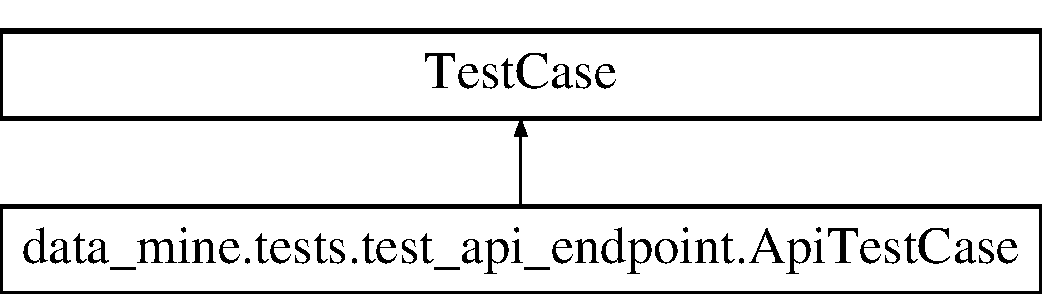
\includegraphics[height=2.000000cm]{classdata__mine_1_1tests_1_1test__api__endpoint_1_1_api_test_case}
\end{center}
\end{figure}
\subsection*{Public Member Functions}
\begin{DoxyCompactItemize}
\item 
\mbox{\Hypertarget{classdata__mine_1_1tests_1_1test__api__endpoint_1_1_api_test_case_af9d2687e79fb283887b9c0a3f3425942}\label{classdata__mine_1_1tests_1_1test__api__endpoint_1_1_api_test_case_af9d2687e79fb283887b9c0a3f3425942}} 
def {\bfseries setup} (self)
\item 
\mbox{\Hypertarget{classdata__mine_1_1tests_1_1test__api__endpoint_1_1_api_test_case_a24c01ec1676be7417914a68d3545380e}\label{classdata__mine_1_1tests_1_1test__api__endpoint_1_1_api_test_case_a24c01ec1676be7417914a68d3545380e}} 
def {\bfseries test\+\_\+api\+\_\+get} (self)
\end{DoxyCompactItemize}


The documentation for this class was generated from the following file\+:\begin{DoxyCompactItemize}
\item 
backend/data\+\_\+mine/tests/test\+\_\+api\+\_\+endpoint.\+py\end{DoxyCompactItemize}

\hypertarget{classstocks_1_1tests_1_1_code_style_test_case}{}\section{stocks.\+tests.\+Code\+Style\+Test\+Case Class Reference}
\label{classstocks_1_1tests_1_1_code_style_test_case}\index{stocks.\+tests.\+Code\+Style\+Test\+Case@{stocks.\+tests.\+Code\+Style\+Test\+Case}}
Inheritance diagram for stocks.\+tests.\+Code\+Style\+Test\+Case\+:\begin{figure}[H]
\begin{center}
\leavevmode
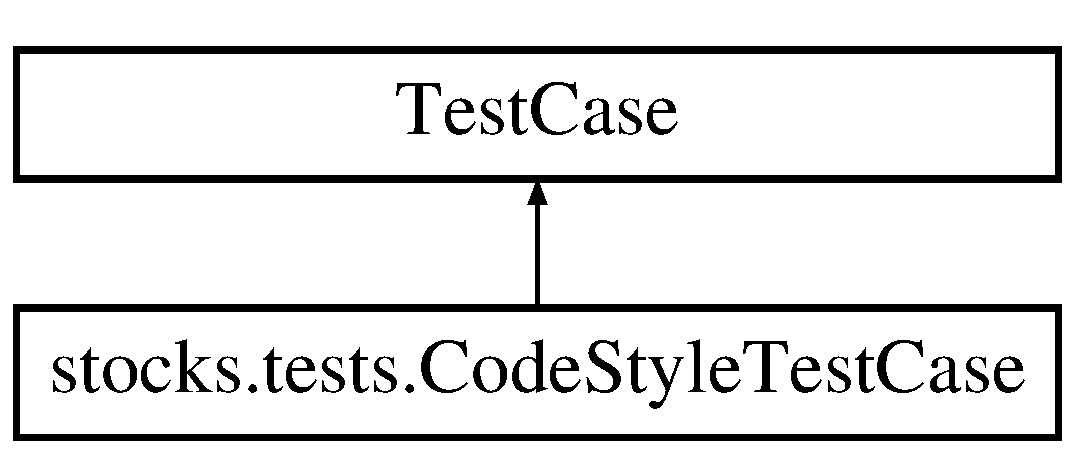
\includegraphics[height=2.000000cm]{classstocks_1_1tests_1_1_code_style_test_case}
\end{center}
\end{figure}
\subsection*{Public Member Functions}
\begin{DoxyCompactItemize}
\item 
def \mbox{\hyperlink{classstocks_1_1tests_1_1_code_style_test_case_a132cc200ec770fe6a050aadcce5032b2}{test\+\_\+pep8}} (self)
\end{DoxyCompactItemize}


\subsection{Member Function Documentation}
\mbox{\Hypertarget{classstocks_1_1tests_1_1_code_style_test_case_a132cc200ec770fe6a050aadcce5032b2}\label{classstocks_1_1tests_1_1_code_style_test_case_a132cc200ec770fe6a050aadcce5032b2}} 
\index{stocks\+::tests\+::\+Code\+Style\+Test\+Case@{stocks\+::tests\+::\+Code\+Style\+Test\+Case}!test\+\_\+pep8@{test\+\_\+pep8}}
\index{test\+\_\+pep8@{test\+\_\+pep8}!stocks\+::tests\+::\+Code\+Style\+Test\+Case@{stocks\+::tests\+::\+Code\+Style\+Test\+Case}}
\subsubsection{\texorpdfstring{test\+\_\+pep8()}{test\_pep8()}}
{\footnotesize\ttfamily def stocks.\+tests.\+Code\+Style\+Test\+Case.\+test\+\_\+pep8 (\begin{DoxyParamCaption}\item[{}]{self }\end{DoxyParamCaption})}

\begin{DoxyVerb}Checks if all files in test_files are PEP8 compliant.
\end{DoxyVerb}
 

The documentation for this class was generated from the following file\+:\begin{DoxyCompactItemize}
\item 
backend/stocks/tests.\+py\end{DoxyCompactItemize}

\hypertarget{classdata__mine_1_1tests_1_1test__companies_1_1_company_test_case}{}\section{data\+\_\+mine.\+tests.\+test\+\_\+companies.\+Company\+Test\+Case Class Reference}
\label{classdata__mine_1_1tests_1_1test__companies_1_1_company_test_case}\index{data\+\_\+mine.\+tests.\+test\+\_\+companies.\+Company\+Test\+Case@{data\+\_\+mine.\+tests.\+test\+\_\+companies.\+Company\+Test\+Case}}
Inheritance diagram for data\+\_\+mine.\+tests.\+test\+\_\+companies.\+Company\+Test\+Case\+:\begin{figure}[H]
\begin{center}
\leavevmode
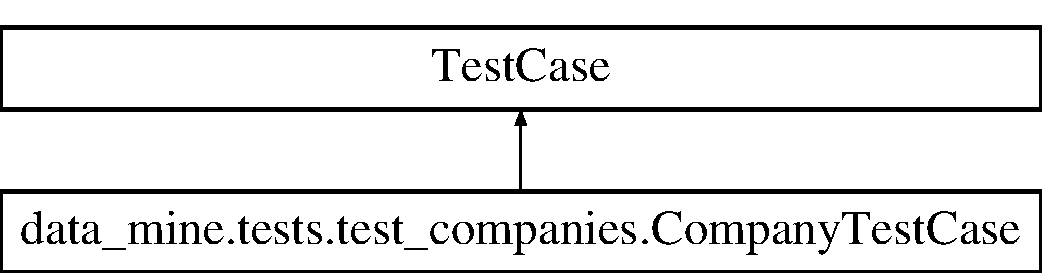
\includegraphics[height=2.000000cm]{classdata__mine_1_1tests_1_1test__companies_1_1_company_test_case}
\end{center}
\end{figure}
\subsection*{Public Member Functions}
\begin{DoxyCompactItemize}
\item 
\mbox{\Hypertarget{classdata__mine_1_1tests_1_1test__companies_1_1_company_test_case_a06558a63be4757213f6ec4ef91ee2f41}\label{classdata__mine_1_1tests_1_1test__companies_1_1_company_test_case_a06558a63be4757213f6ec4ef91ee2f41}} 
def {\bfseries set\+Up\+Test\+Data} (self)
\item 
\mbox{\Hypertarget{classdata__mine_1_1tests_1_1test__companies_1_1_company_test_case_a94a2ce9c364c871fdb57db80bf6fdca5}\label{classdata__mine_1_1tests_1_1test__companies_1_1_company_test_case_a94a2ce9c364c871fdb57db80bf6fdca5}} 
def {\bfseries test\+\_\+company\+\_\+create} (self)
\end{DoxyCompactItemize}


The documentation for this class was generated from the following file\+:\begin{DoxyCompactItemize}
\item 
backend/data\+\_\+mine/tests/test\+\_\+companies.\+py\end{DoxyCompactItemize}

\hypertarget{classweb__service_1_1_data_1_1_data}{}\section{web\+\_\+service.\+Data.\+Data Class Reference}
\label{classweb__service_1_1_data_1_1_data}\index{web\+\_\+service.\+Data.\+Data@{web\+\_\+service.\+Data.\+Data}}
\subsection*{Public Member Functions}
\begin{DoxyCompactItemize}
\item 
def \mbox{\hyperlink{classweb__service_1_1_data_1_1_data_a8f843b77e0a7cf2d263a2f28696c4f58}{\+\_\+\+\_\+init\+\_\+\+\_\+}} (self)
\item 
def \mbox{\hyperlink{classweb__service_1_1_data_1_1_data_ae5f263f0a89d3a6b2bbbcac8d590f4cc}{get\+\_\+data}} (self, input\+\_\+data)
\end{DoxyCompactItemize}


\subsection{Constructor \& Destructor Documentation}
\mbox{\Hypertarget{classweb__service_1_1_data_1_1_data_a8f843b77e0a7cf2d263a2f28696c4f58}\label{classweb__service_1_1_data_1_1_data_a8f843b77e0a7cf2d263a2f28696c4f58}} 
\index{web\+\_\+service\+::\+Data\+::\+Data@{web\+\_\+service\+::\+Data\+::\+Data}!\+\_\+\+\_\+init\+\_\+\+\_\+@{\+\_\+\+\_\+init\+\_\+\+\_\+}}
\index{\+\_\+\+\_\+init\+\_\+\+\_\+@{\+\_\+\+\_\+init\+\_\+\+\_\+}!web\+\_\+service\+::\+Data\+::\+Data@{web\+\_\+service\+::\+Data\+::\+Data}}
\subsubsection{\texorpdfstring{\+\_\+\+\_\+init\+\_\+\+\_\+()}{\_\_init\_\_()}}
{\footnotesize\ttfamily def web\+\_\+service.\+Data.\+Data.\+\_\+\+\_\+init\+\_\+\+\_\+ (\begin{DoxyParamCaption}\item[{}]{self }\end{DoxyParamCaption})}

\begin{DoxyVerb}    Data class to connect to ML studio web service
    _api_key: API to ML studio web service
    _url: URL to connect to ML studio
\end{DoxyVerb}
 

\subsection{Member Function Documentation}
\mbox{\Hypertarget{classweb__service_1_1_data_1_1_data_ae5f263f0a89d3a6b2bbbcac8d590f4cc}\label{classweb__service_1_1_data_1_1_data_ae5f263f0a89d3a6b2bbbcac8d590f4cc}} 
\index{web\+\_\+service\+::\+Data\+::\+Data@{web\+\_\+service\+::\+Data\+::\+Data}!get\+\_\+data@{get\+\_\+data}}
\index{get\+\_\+data@{get\+\_\+data}!web\+\_\+service\+::\+Data\+::\+Data@{web\+\_\+service\+::\+Data\+::\+Data}}
\subsubsection{\texorpdfstring{get\+\_\+data()}{get\_data()}}
{\footnotesize\ttfamily def web\+\_\+service.\+Data.\+Data.\+get\+\_\+data (\begin{DoxyParamCaption}\item[{}]{self,  }\item[{}]{input\+\_\+data }\end{DoxyParamCaption})}

\begin{DoxyVerb}   Get the prediction result from Azure Machine Learning Studio
   input_data: input data to parse into ML webservice to run experiment
\end{DoxyVerb}
 

The documentation for this class was generated from the following file\+:\begin{DoxyCompactItemize}
\item 
web\+\_\+service/Data.\+py\end{DoxyCompactItemize}

\hypertarget{classweb__service_1_1get__data_1_1_data}{}\section{web\+\_\+service.\+get\+\_\+data.\+Data Class Reference}
\label{classweb__service_1_1get__data_1_1_data}\index{web\+\_\+service.\+get\+\_\+data.\+Data@{web\+\_\+service.\+get\+\_\+data.\+Data}}
\subsection*{Public Member Functions}
\begin{DoxyCompactItemize}
\item 
\mbox{\Hypertarget{classweb__service_1_1get__data_1_1_data_af313165f79ee0dbf27f6ed24ca775d50}\label{classweb__service_1_1get__data_1_1_data_af313165f79ee0dbf27f6ed24ca775d50}} 
def {\bfseries \+\_\+\+\_\+init\+\_\+\+\_\+} (self)
\item 
\mbox{\Hypertarget{classweb__service_1_1get__data_1_1_data_a0db42a21a20452264f21878ed252e9f0}\label{classweb__service_1_1get__data_1_1_data_a0db42a21a20452264f21878ed252e9f0}} 
def {\bfseries get\+\_\+data} (input)
\end{DoxyCompactItemize}


The documentation for this class was generated from the following file\+:\begin{DoxyCompactItemize}
\item 
web\+\_\+service/get\+\_\+data.\+py\end{DoxyCompactItemize}

\hypertarget{classdata__mine_1_1apps_1_1_data_mine_config}{}\section{data\+\_\+mine.\+apps.\+Data\+Mine\+Config Class Reference}
\label{classdata__mine_1_1apps_1_1_data_mine_config}\index{data\+\_\+mine.\+apps.\+Data\+Mine\+Config@{data\+\_\+mine.\+apps.\+Data\+Mine\+Config}}
Inheritance diagram for data\+\_\+mine.\+apps.\+Data\+Mine\+Config\+:\begin{figure}[H]
\begin{center}
\leavevmode
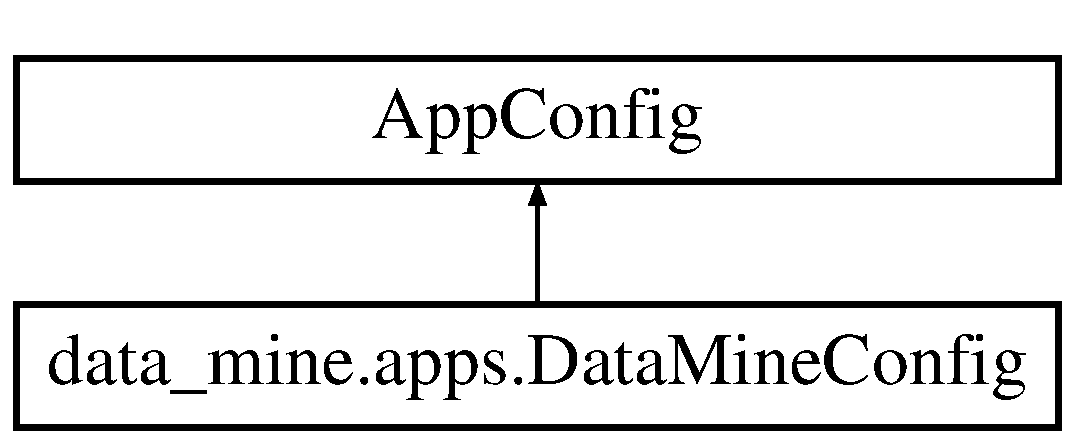
\includegraphics[height=2.000000cm]{classdata__mine_1_1apps_1_1_data_mine_config}
\end{center}
\end{figure}
\subsection*{Static Public Attributes}
\begin{DoxyCompactItemize}
\item 
\mbox{\Hypertarget{classdata__mine_1_1apps_1_1_data_mine_config_a458cf75e478f98cc2882951a3b52690c}\label{classdata__mine_1_1apps_1_1_data_mine_config_a458cf75e478f98cc2882951a3b52690c}} 
string {\bfseries name} = \textquotesingle{}data\+\_\+mine\textquotesingle{}
\end{DoxyCompactItemize}


The documentation for this class was generated from the following file\+:\begin{DoxyCompactItemize}
\item 
backend/data\+\_\+mine/apps.\+py\end{DoxyCompactItemize}

\hypertarget{classstocks_1_1utilities_1_1_experiment_manager}{}\section{stocks.\+utilities.\+Experiment\+Manager Class Reference}
\label{classstocks_1_1utilities_1_1_experiment_manager}\index{stocks.\+utilities.\+Experiment\+Manager@{stocks.\+utilities.\+Experiment\+Manager}}
\subsection*{Static Public Member Functions}
\begin{DoxyCompactItemize}
\item 
def \mbox{\hyperlink{classstocks_1_1utilities_1_1_experiment_manager_a0cddeda4b8d32587b7160be9b33ace52}{run\+\_\+experiment}} (ticker)
\end{DoxyCompactItemize}


\subsection{Detailed Description}
\begin{DoxyVerb}Utility class to hold functions related to experiments.
\end{DoxyVerb}
 

\subsection{Member Function Documentation}
\mbox{\Hypertarget{classstocks_1_1utilities_1_1_experiment_manager_a0cddeda4b8d32587b7160be9b33ace52}\label{classstocks_1_1utilities_1_1_experiment_manager_a0cddeda4b8d32587b7160be9b33ace52}} 
\index{stocks\+::utilities\+::\+Experiment\+Manager@{stocks\+::utilities\+::\+Experiment\+Manager}!run\+\_\+experiment@{run\+\_\+experiment}}
\index{run\+\_\+experiment@{run\+\_\+experiment}!stocks\+::utilities\+::\+Experiment\+Manager@{stocks\+::utilities\+::\+Experiment\+Manager}}
\subsubsection{\texorpdfstring{run\+\_\+experiment()}{run\_experiment()}}
{\footnotesize\ttfamily def stocks.\+utilities.\+Experiment\+Manager.\+run\+\_\+experiment (\begin{DoxyParamCaption}\item[{}]{ticker }\end{DoxyParamCaption})\hspace{0.3cm}{\ttfamily [static]}}

\begin{DoxyVerb}Run experiment for given ticker and returns list of experiment results
packed in JSON format.
Fails if company doesn't exist in database.
:param ticker: Ticker symbol to run experiment
:return: JSON containing list of experiment results.
 -1 if company is not found in database.
\end{DoxyVerb}
 

The documentation for this class was generated from the following file\+:\begin{DoxyCompactItemize}
\item 
backend/stocks/utilities.\+py\end{DoxyCompactItemize}

\hypertarget{classdata__mine_1_1_extract_tickers_1_1_extract_tickers}{}\section{data\+\_\+mine.\+Extract\+Tickers.\+Extract\+Tickers Class Reference}
\label{classdata__mine_1_1_extract_tickers_1_1_extract_tickers}\index{data\+\_\+mine.\+Extract\+Tickers.\+Extract\+Tickers@{data\+\_\+mine.\+Extract\+Tickers.\+Extract\+Tickers}}
\subsection*{Public Member Functions}
\begin{DoxyCompactItemize}
\item 
\mbox{\Hypertarget{classdata__mine_1_1_extract_tickers_1_1_extract_tickers_afa1e390dcab8f12d4a21735d3adf28ad}\label{classdata__mine_1_1_extract_tickers_1_1_extract_tickers_afa1e390dcab8f12d4a21735d3adf28ad}} 
def {\bfseries read\+\_\+csv} (self)
\item 
\mbox{\Hypertarget{classdata__mine_1_1_extract_tickers_1_1_extract_tickers_aa8425c36c82a649fd313a4001eaf9583}\label{classdata__mine_1_1_extract_tickers_1_1_extract_tickers_aa8425c36c82a649fd313a4001eaf9583}} 
def {\bfseries get\+\_\+tickers} (self)
\end{DoxyCompactItemize}
\subsection*{Static Public Attributes}
\begin{DoxyCompactItemize}
\item 
\mbox{\Hypertarget{classdata__mine_1_1_extract_tickers_1_1_extract_tickers_aa6fda0b0db87b9896190326cc3d79c9c}\label{classdata__mine_1_1_extract_tickers_1_1_extract_tickers_aa6fda0b0db87b9896190326cc3d79c9c}} 
string {\bfseries C\+SV} = \char`\"{}tickers.\+csv\char`\"{}
\end{DoxyCompactItemize}


The documentation for this class was generated from the following file\+:\begin{DoxyCompactItemize}
\item 
backend/data\+\_\+mine/Extract\+Tickers.\+py\end{DoxyCompactItemize}

\hypertarget{classdata__mine_1_1_insert_tickers_1_1_insert_tickers}{}\section{data\+\_\+mine.\+Insert\+Tickers.\+Insert\+Tickers Class Reference}
\label{classdata__mine_1_1_insert_tickers_1_1_insert_tickers}\index{data\+\_\+mine.\+Insert\+Tickers.\+Insert\+Tickers@{data\+\_\+mine.\+Insert\+Tickers.\+Insert\+Tickers}}
\subsection*{Public Member Functions}
\begin{DoxyCompactItemize}
\item 
\mbox{\Hypertarget{classdata__mine_1_1_insert_tickers_1_1_insert_tickers_a3b0d7675445fcbb17a31ab3214f471e0}\label{classdata__mine_1_1_insert_tickers_1_1_insert_tickers_a3b0d7675445fcbb17a31ab3214f471e0}} 
def {\bfseries \+\_\+\+\_\+init\+\_\+\+\_\+} (self, custom=\textquotesingle{}all\textquotesingle{}, all\+\_\+tickers=False)
\item 
\mbox{\Hypertarget{classdata__mine_1_1_insert_tickers_1_1_insert_tickers_a6090e2f692effe8e712840453ebcd5ff}\label{classdata__mine_1_1_insert_tickers_1_1_insert_tickers_a6090e2f692effe8e712840453ebcd5ff}} 
def {\bfseries get\+\_\+datelist} (self, num\+\_\+dates)
\item 
\mbox{\Hypertarget{classdata__mine_1_1_insert_tickers_1_1_insert_tickers_ab69431f5b0fbeffdddd33e57d908199a}\label{classdata__mine_1_1_insert_tickers_1_1_insert_tickers_ab69431f5b0fbeffdddd33e57d908199a}} 
def {\bfseries get\+\_\+custom\+\_\+ticker} (self, ticker)
\item 
\mbox{\Hypertarget{classdata__mine_1_1_insert_tickers_1_1_insert_tickers_a94721312a4859670da22037a475a8221}\label{classdata__mine_1_1_insert_tickers_1_1_insert_tickers_a94721312a4859670da22037a475a8221}} 
def {\bfseries get\+\_\+all\+\_\+tickers} (self)
\item 
\mbox{\Hypertarget{classdata__mine_1_1_insert_tickers_1_1_insert_tickers_ab9ab73c2a11c89792504f2b2e92b3f01}\label{classdata__mine_1_1_insert_tickers_1_1_insert_tickers_ab9ab73c2a11c89792504f2b2e92b3f01}} 
def {\bfseries run} (self, num\+\_\+dates, tickers=None)
\item 
def \mbox{\hyperlink{classdata__mine_1_1_insert_tickers_1_1_insert_tickers_a817932df15b0d8af46ccb0f3b3f009be}{post\+\_\+to\+\_\+api}} (self, ticker\+\_\+list, date\+\_\+list)
\end{DoxyCompactItemize}
\subsection*{Public Attributes}
\begin{DoxyCompactItemize}
\item 
\mbox{\Hypertarget{classdata__mine_1_1_insert_tickers_1_1_insert_tickers_ac3446c530e26a42c28900c1440c39098}\label{classdata__mine_1_1_insert_tickers_1_1_insert_tickers_ac3446c530e26a42c28900c1440c39098}} 
{\bfseries mine}
\item 
\mbox{\Hypertarget{classdata__mine_1_1_insert_tickers_1_1_insert_tickers_a0787a916b4f64dfecda45affbf3b992d}\label{classdata__mine_1_1_insert_tickers_1_1_insert_tickers_a0787a916b4f64dfecda45affbf3b992d}} 
{\bfseries custom}
\item 
\mbox{\Hypertarget{classdata__mine_1_1_insert_tickers_1_1_insert_tickers_aa9a83795442e916a9cd789bf114d4d48}\label{classdata__mine_1_1_insert_tickers_1_1_insert_tickers_aa9a83795442e916a9cd789bf114d4d48}} 
{\bfseries all}
\end{DoxyCompactItemize}


\subsection{Member Function Documentation}
\mbox{\Hypertarget{classdata__mine_1_1_insert_tickers_1_1_insert_tickers_a817932df15b0d8af46ccb0f3b3f009be}\label{classdata__mine_1_1_insert_tickers_1_1_insert_tickers_a817932df15b0d8af46ccb0f3b3f009be}} 
\index{data\+\_\+mine\+::\+Insert\+Tickers\+::\+Insert\+Tickers@{data\+\_\+mine\+::\+Insert\+Tickers\+::\+Insert\+Tickers}!post\+\_\+to\+\_\+api@{post\+\_\+to\+\_\+api}}
\index{post\+\_\+to\+\_\+api@{post\+\_\+to\+\_\+api}!data\+\_\+mine\+::\+Insert\+Tickers\+::\+Insert\+Tickers@{data\+\_\+mine\+::\+Insert\+Tickers\+::\+Insert\+Tickers}}
\subsubsection{\texorpdfstring{post\+\_\+to\+\_\+api()}{post\_to\_api()}}
{\footnotesize\ttfamily def data\+\_\+mine.\+Insert\+Tickers.\+Insert\+Tickers.\+post\+\_\+to\+\_\+api (\begin{DoxyParamCaption}\item[{}]{self,  }\item[{}]{ticker\+\_\+list,  }\item[{}]{date\+\_\+list }\end{DoxyParamCaption})}

\begin{DoxyVerb}Insert custom ticker to /stocks
    ticker_list: list of tickers
    date_list: list of dates for a range
\end{DoxyVerb}
 

The documentation for this class was generated from the following file\+:\begin{DoxyCompactItemize}
\item 
backend/data\+\_\+mine/Insert\+Tickers.\+py\end{DoxyCompactItemize}

\hypertarget{classdata__mine_1_1tests_1_1test__insert_tickers_1_1_insert_tickers_test_case}{}\section{data\+\_\+mine.\+tests.\+test\+\_\+insert\+Tickers.\+Insert\+Tickers\+Test\+Case Class Reference}
\label{classdata__mine_1_1tests_1_1test__insert_tickers_1_1_insert_tickers_test_case}\index{data\+\_\+mine.\+tests.\+test\+\_\+insert\+Tickers.\+Insert\+Tickers\+Test\+Case@{data\+\_\+mine.\+tests.\+test\+\_\+insert\+Tickers.\+Insert\+Tickers\+Test\+Case}}
Inheritance diagram for data\+\_\+mine.\+tests.\+test\+\_\+insert\+Tickers.\+Insert\+Tickers\+Test\+Case\+:\begin{figure}[H]
\begin{center}
\leavevmode
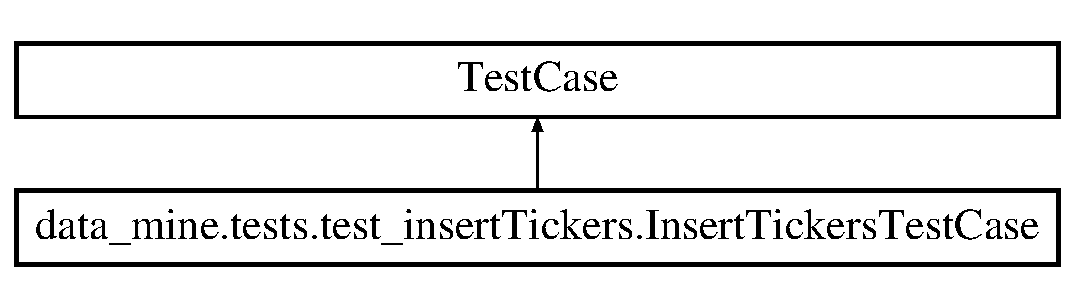
\includegraphics[height=2.000000cm]{classdata__mine_1_1tests_1_1test__insert_tickers_1_1_insert_tickers_test_case}
\end{center}
\end{figure}
\subsection*{Public Member Functions}
\begin{DoxyCompactItemize}
\item 
\mbox{\Hypertarget{classdata__mine_1_1tests_1_1test__insert_tickers_1_1_insert_tickers_test_case_ae5d0c297cb83611a4343f9872a8c7b82}\label{classdata__mine_1_1tests_1_1test__insert_tickers_1_1_insert_tickers_test_case_ae5d0c297cb83611a4343f9872a8c7b82}} 
def {\bfseries test\+\_\+get\+\_\+custom\+\_\+ticker} (self)
\end{DoxyCompactItemize}
\subsection*{Static Public Attributes}
\begin{DoxyCompactItemize}
\item 
\mbox{\Hypertarget{classdata__mine_1_1tests_1_1test__insert_tickers_1_1_insert_tickers_test_case_a3f8b8b39f7e4db787ecaf064c8ca2c00}\label{classdata__mine_1_1tests_1_1test__insert_tickers_1_1_insert_tickers_test_case_a3f8b8b39f7e4db787ecaf064c8ca2c00}} 
string {\bfseries pdg\+\_\+link} = \textquotesingle{}http\+://prodigal-\/ml.\+us-\/east-\/2.elasticbeanstalk.\+com/stocks/\textquotesingle{}
\item 
\mbox{\Hypertarget{classdata__mine_1_1tests_1_1test__insert_tickers_1_1_insert_tickers_test_case_ab725e74096b9511abf7694c7e830513c}\label{classdata__mine_1_1tests_1_1test__insert_tickers_1_1_insert_tickers_test_case_ab725e74096b9511abf7694c7e830513c}} 
{\bfseries it} = \mbox{\hyperlink{classdata__mine_1_1_insert_tickers_1_1_insert_tickers}{Insert\+Tickers}}()
\end{DoxyCompactItemize}


The documentation for this class was generated from the following file\+:\begin{DoxyCompactItemize}
\item 
backend/data\+\_\+mine/tests/test\+\_\+insert\+Tickers.\+py\end{DoxyCompactItemize}

\hypertarget{classstocks_1_1serializers_1_1_stock_serializer_1_1_meta}{}\section{stocks.\+serializers.\+Stock\+Serializer.\+Meta Class Reference}
\label{classstocks_1_1serializers_1_1_stock_serializer_1_1_meta}\index{stocks.\+serializers.\+Stock\+Serializer.\+Meta@{stocks.\+serializers.\+Stock\+Serializer.\+Meta}}
\subsection*{Static Public Attributes}
\begin{DoxyCompactItemize}
\item 
\mbox{\Hypertarget{classstocks_1_1serializers_1_1_stock_serializer_1_1_meta_a6af5e3bff413e445333d51390b26cbc6}\label{classstocks_1_1serializers_1_1_stock_serializer_1_1_meta_a6af5e3bff413e445333d51390b26cbc6}} 
{\bfseries model} = \mbox{\hyperlink{classstocks_1_1models_1_1_stock}{Stock}}
\item 
tuple {\bfseries fields}
\end{DoxyCompactItemize}


\subsection{Member Data Documentation}
\mbox{\Hypertarget{classstocks_1_1serializers_1_1_stock_serializer_1_1_meta_aa606dd7e7d5d18b676c8682055f764c1}\label{classstocks_1_1serializers_1_1_stock_serializer_1_1_meta_aa606dd7e7d5d18b676c8682055f764c1}} 
\index{stocks\+::serializers\+::\+Stock\+Serializer\+::\+Meta@{stocks\+::serializers\+::\+Stock\+Serializer\+::\+Meta}!fields@{fields}}
\index{fields@{fields}!stocks\+::serializers\+::\+Stock\+Serializer\+::\+Meta@{stocks\+::serializers\+::\+Stock\+Serializer\+::\+Meta}}
\subsubsection{\texorpdfstring{fields}{fields}}
{\footnotesize\ttfamily tuple stocks.\+serializers.\+Stock\+Serializer.\+Meta.\+fields\hspace{0.3cm}{\ttfamily [static]}}

{\bfseries Initial value\+:}
\begin{DoxyCode}
=  (\textcolor{stringliteral}{"ticker"}, \textcolor{stringliteral}{"high"}, \textcolor{stringliteral}{"low"},
                  \textcolor{stringliteral}{"opening"}, \textcolor{stringliteral}{"closing"}, \textcolor{stringliteral}{"volume"}, \textcolor{stringliteral}{"date"})
\end{DoxyCode}


The documentation for this class was generated from the following file\+:\begin{DoxyCompactItemize}
\item 
backend/stocks/serializers.\+py\end{DoxyCompactItemize}

\hypertarget{classsnippets_1_1models_1_1_snippet_1_1_meta}{}\section{snippets.\+models.\+Snippet.\+Meta Class Reference}
\label{classsnippets_1_1models_1_1_snippet_1_1_meta}\index{snippets.\+models.\+Snippet.\+Meta@{snippets.\+models.\+Snippet.\+Meta}}
\subsection*{Static Public Attributes}
\begin{DoxyCompactItemize}
\item 
\mbox{\Hypertarget{classsnippets_1_1models_1_1_snippet_1_1_meta_a5c59dd90a327bd10f7bfa725529f7423}\label{classsnippets_1_1models_1_1_snippet_1_1_meta_a5c59dd90a327bd10f7bfa725529f7423}} 
tuple {\bfseries ordering} = (\textquotesingle{}created\textquotesingle{}, )
\end{DoxyCompactItemize}


The documentation for this class was generated from the following file\+:\begin{DoxyCompactItemize}
\item 
spike/hwin16/mysite/snippets/models.\+py\end{DoxyCompactItemize}

\hypertarget{classsnippets_1_1serializers_1_1_snippet_serializer_1_1_meta}{}\section{snippets.\+serializers.\+Snippet\+Serializer.\+Meta Class Reference}
\label{classsnippets_1_1serializers_1_1_snippet_serializer_1_1_meta}\index{snippets.\+serializers.\+Snippet\+Serializer.\+Meta@{snippets.\+serializers.\+Snippet\+Serializer.\+Meta}}
\subsection*{Static Public Attributes}
\begin{DoxyCompactItemize}
\item 
\mbox{\Hypertarget{classsnippets_1_1serializers_1_1_snippet_serializer_1_1_meta_a015ad7c59459713a3f7c2c3d2dd5834f}\label{classsnippets_1_1serializers_1_1_snippet_serializer_1_1_meta_a015ad7c59459713a3f7c2c3d2dd5834f}} 
{\bfseries model} = \mbox{\hyperlink{classsnippets_1_1models_1_1_snippet}{Snippet}}
\item 
\mbox{\Hypertarget{classsnippets_1_1serializers_1_1_snippet_serializer_1_1_meta_ad6280ba8307386556c7e79538405b7f6}\label{classsnippets_1_1serializers_1_1_snippet_serializer_1_1_meta_ad6280ba8307386556c7e79538405b7f6}} 
tuple {\bfseries fields} = (\textquotesingle{}id\textquotesingle{}, \textquotesingle{}title\textquotesingle{}, \textquotesingle{}code\textquotesingle{}, \textquotesingle{}linenos\textquotesingle{}, \textquotesingle{}language\textquotesingle{}, \textquotesingle{}style\textquotesingle{})
\end{DoxyCompactItemize}


The documentation for this class was generated from the following file\+:\begin{DoxyCompactItemize}
\item 
spike/hwin16/mysite/snippets/serializers.\+py\end{DoxyCompactItemize}

\hypertarget{classsnippets_1_1migrations_1_10001__initial_1_1_migration}{}\section{snippets.\+migrations.0001\+\_\+initial.Migration Class Reference}
\label{classsnippets_1_1migrations_1_10001__initial_1_1_migration}\index{snippets.\+migrations.\+0001\+\_\+initial.\+Migration@{snippets.\+migrations.\+0001\+\_\+initial.\+Migration}}
Inheritance diagram for snippets.\+migrations.0001\+\_\+initial.Migration\+:\begin{figure}[H]
\begin{center}
\leavevmode
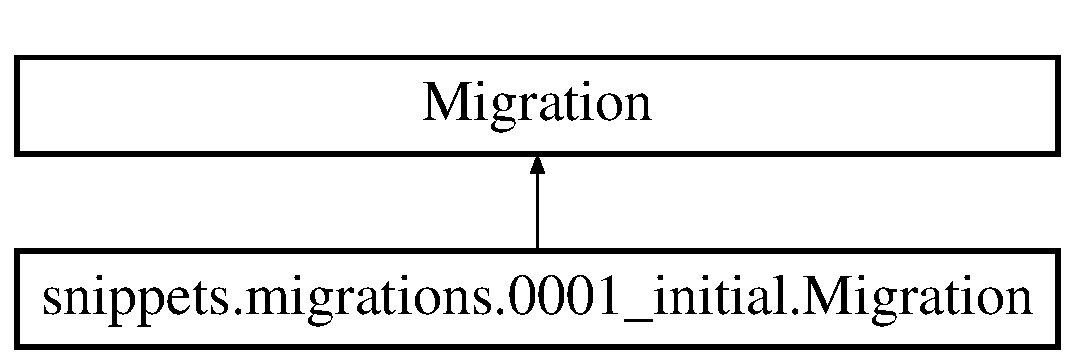
\includegraphics[height=2.000000cm]{classsnippets_1_1migrations_1_10001__initial_1_1_migration}
\end{center}
\end{figure}
\subsection*{Static Public Attributes}
\begin{DoxyCompactItemize}
\item 
\mbox{\Hypertarget{classsnippets_1_1migrations_1_10001__initial_1_1_migration_a15710109783bc33a9894518160304f10}\label{classsnippets_1_1migrations_1_10001__initial_1_1_migration_a15710109783bc33a9894518160304f10}} 
bool {\bfseries initial} = True
\item 
list {\bfseries dependencies}
\item 
list {\bfseries operations}
\end{DoxyCompactItemize}


\subsection{Member Data Documentation}
\mbox{\Hypertarget{classsnippets_1_1migrations_1_10001__initial_1_1_migration_a8dcd961f450c0f66f326ce9daef450f5}\label{classsnippets_1_1migrations_1_10001__initial_1_1_migration_a8dcd961f450c0f66f326ce9daef450f5}} 
\index{snippets\+::migrations\+::0001\+\_\+initial\+::\+Migration@{snippets\+::migrations\+::0001\+\_\+initial\+::\+Migration}!dependencies@{dependencies}}
\index{dependencies@{dependencies}!snippets\+::migrations\+::0001\+\_\+initial\+::\+Migration@{snippets\+::migrations\+::0001\+\_\+initial\+::\+Migration}}
\subsubsection{\texorpdfstring{dependencies}{dependencies}}
{\footnotesize\ttfamily list snippets.\+migrations.\+0001\+\_\+initial.\+Migration.\+dependencies\hspace{0.3cm}{\ttfamily [static]}}

{\bfseries Initial value\+:}
\begin{DoxyCode}
=  [
    ]
\end{DoxyCode}
\mbox{\Hypertarget{classsnippets_1_1migrations_1_10001__initial_1_1_migration_af800dea6df4f70c866af5cf5ec04d9ca}\label{classsnippets_1_1migrations_1_10001__initial_1_1_migration_af800dea6df4f70c866af5cf5ec04d9ca}} 
\index{snippets\+::migrations\+::0001\+\_\+initial\+::\+Migration@{snippets\+::migrations\+::0001\+\_\+initial\+::\+Migration}!operations@{operations}}
\index{operations@{operations}!snippets\+::migrations\+::0001\+\_\+initial\+::\+Migration@{snippets\+::migrations\+::0001\+\_\+initial\+::\+Migration}}
\subsubsection{\texorpdfstring{operations}{operations}}
{\footnotesize\ttfamily list snippets.\+migrations.\+0001\+\_\+initial.\+Migration.\+operations\hspace{0.3cm}{\ttfamily [static]}}

{\bfseries Initial value\+:}
\begin{DoxyCode}
=  [
        migrations.CreateModel(
            name=\textcolor{stringliteral}{'Snippet'},
            fields=[
                (\textcolor{stringliteral}{'id'}, models.AutoField(auto\_created=\textcolor{keyword}{True}, primary\_key=\textcolor{keyword}{True}, serialize=\textcolor{keyword}{False}, verbose\_name=\textcolor{stringliteral}{
      'ID'})),
                (\textcolor{stringliteral}{'created'}, models.DateTimeField(auto\_now\_add=\textcolor{keyword}{True})),
                (\textcolor{stringliteral}{'title'}, models.CharField(blank=\textcolor{keyword}{True}, default=\textcolor{stringliteral}{''}, max\_length=100)),
                (\textcolor{stringliteral}{'code'}, models.TextField()),
                (\textcolor{stringliteral}{'linenos'}, models.BooleanField(default=\textcolor{keyword}{False})),
                (\textcolor{stringliteral}{'language'}, models.CharField(choices=[(\textcolor{stringliteral}{'abap'}, \textcolor{stringliteral}{'ABAP'}), (\textcolor{stringliteral}{'abnf'}, \textcolor{stringliteral}{'ABNF'}), (\textcolor{stringliteral}{'ada'}, \textcolor{stringliteral}{'Ada'}), 
      (\textcolor{stringliteral}{'adl'}, \textcolor{stringliteral}{'ADL'}), (\textcolor{stringliteral}{'agda'}, \textcolor{stringliteral}{'Agda'}), (\textcolor{stringliteral}{'aheui'}, \textcolor{stringliteral}{'Aheui'}), (\textcolor{stringliteral}{'ahk'}, \textcolor{stringliteral}{'autohotkey'}), (\textcolor{stringliteral}{'alloy'}, \textcolor{stringliteral}{'Alloy'}), (\textcolor{stringliteral}{'ampl'}, \textcolor{stringliteral}{'
      Ampl'}), (\textcolor{stringliteral}{'antlr'}, \textcolor{stringliteral}{'ANTLR'}), (\textcolor{stringliteral}{'antlr-as'}, \textcolor{stringliteral}{'ANTLR With ActionScript Target'}), (\textcolor{stringliteral}{'antlr-cpp'}, \textcolor{stringliteral}{'ANTLR With CPP
       Target'}), (\textcolor{stringliteral}{'antlr-csharp'}, \textcolor{stringliteral}{'ANTLR With C# Target'}), (\textcolor{stringliteral}{'antlr-java'}, \textcolor{stringliteral}{'ANTLR With Java Target'}), (\textcolor{stringliteral}{'antlr-objc'}, \textcolor{stringliteral}{'
      ANTLR With ObjectiveC Target'}), (\textcolor{stringliteral}{'antlr-perl'}, \textcolor{stringliteral}{'ANTLR With Perl Target'}), (\textcolor{stringliteral}{'antlr-python'}, \textcolor{stringliteral}{'ANTLR With Python
       Target'}), (\textcolor{stringliteral}{'antlr-ruby'}, \textcolor{stringliteral}{'ANTLR With Ruby Target'}), (\textcolor{stringliteral}{'apacheconf'}, \textcolor{stringliteral}{'ApacheConf'}), (\textcolor{stringliteral}{'apl'}, \textcolor{stringliteral}{'APL'}), (\textcolor{stringliteral}{'
      applescript'}, \textcolor{stringliteral}{'AppleScript'}), (\textcolor{stringliteral}{'arduino'}, \textcolor{stringliteral}{'Arduino'}), (\textcolor{stringliteral}{'as'}, \textcolor{stringliteral}{'ActionScript'}), (\textcolor{stringliteral}{'as3'}, \textcolor{stringliteral}{'ActionScript 3'}), (\textcolor{stringliteral}{'aspectj'}
      , \textcolor{stringliteral}{'AspectJ'}), (\textcolor{stringliteral}{'aspx-cs'}, \textcolor{stringliteral}{'aspx-cs'}), (\textcolor{stringliteral}{'aspx-vb'}, \textcolor{stringliteral}{'aspx-vb'}), (\textcolor{stringliteral}{'asy'}, \textcolor{stringliteral}{'Asymptote'}), (\textcolor{stringliteral}{'at'}, \textcolor{stringliteral}{'AmbientTalk'}), (\textcolor{stringliteral}{
      'autoit'}, \textcolor{stringliteral}{'AutoIt'}), (\textcolor{stringliteral}{'awk'}, \textcolor{stringliteral}{'Awk'}), (\textcolor{stringliteral}{'basemake'}, \textcolor{stringliteral}{'Base Makefile'}), (\textcolor{stringliteral}{'bash'}, \textcolor{stringliteral}{'Bash'}), (\textcolor{stringliteral}{'bat'}, \textcolor{stringliteral}{'Batchfile'}), 
      (\textcolor{stringliteral}{'bbcode'}, \textcolor{stringliteral}{'BBCode'}), (\textcolor{stringliteral}{'bc'}, \textcolor{stringliteral}{'BC'}), (\textcolor{stringliteral}{'befunge'}, \textcolor{stringliteral}{'Befunge'}), (\textcolor{stringliteral}{'bib'}, \textcolor{stringliteral}{'BibTeX'}), (\textcolor{stringliteral}{'blitzbasic'}, \textcolor{stringliteral}{'BlitzBasic'}),
       (\textcolor{stringliteral}{'blitzmax'}, \textcolor{stringliteral}{'BlitzMax'}), (\textcolor{stringliteral}{'bnf'}, \textcolor{stringliteral}{'BNF'}), (\textcolor{stringliteral}{'boo'}, \textcolor{stringliteral}{'Boo'}), (\textcolor{stringliteral}{'boogie'}, \textcolor{stringliteral}{'Boogie'}), (\textcolor{stringliteral}{'brainfuck'}, \textcolor{stringliteral}{'Brainfuck'}),
       (\textcolor{stringliteral}{'bro'}, \textcolor{stringliteral}{'Bro'}), (\textcolor{stringliteral}{'bst'}, \textcolor{stringliteral}{'BST'}), (\textcolor{stringliteral}{'bugs'}, \textcolor{stringliteral}{'BUGS'}), (\textcolor{stringliteral}{'c'}, \textcolor{stringliteral}{'C'}), (\textcolor{stringliteral}{'c-objdump'}, \textcolor{stringliteral}{'c-objdump'}), (\textcolor{stringliteral}{'ca65'}, \textcolor{stringliteral}{'ca65
       assembler'}), (\textcolor{stringliteral}{'cadl'}, \textcolor{stringliteral}{'cADL'}), (\textcolor{stringliteral}{'camkes'}, \textcolor{stringliteral}{'CAmkES'}), (\textcolor{stringliteral}{'capdl'}, \textcolor{stringliteral}{'CapDL'}), (\textcolor{stringliteral}{'capnp'}, \textcolor{stringliteral}{"Cap'n Proto"}), (\textcolor{stringliteral}{'cbmbas'}, \textcolor{stringliteral}{
      'CBM BASIC V2'}), (\textcolor{stringliteral}{'ceylon'}, \textcolor{stringliteral}{'Ceylon'}), (\textcolor{stringliteral}{'cfc'}, \textcolor{stringliteral}{'Coldfusion CFC'}), (\textcolor{stringliteral}{'cfengine3'}, \textcolor{stringliteral}{'CFEngine3'}), (\textcolor{stringliteral}{'cfm'}, \textcolor{stringliteral}{'
      Coldfusion HTML'}), (\textcolor{stringliteral}{'cfs'}, \textcolor{stringliteral}{'cfstatement'}), (\textcolor{stringliteral}{'chai'}, \textcolor{stringliteral}{'ChaiScript'}), (\textcolor{stringliteral}{'chapel'}, \textcolor{stringliteral}{'Chapel'}), (\textcolor{stringliteral}{'cheetah'}, \textcolor{stringliteral}{'Cheetah'}), 
      (\textcolor{stringliteral}{'cirru'}, \textcolor{stringliteral}{'Cirru'}), (\textcolor{stringliteral}{'clay'}, \textcolor{stringliteral}{'Clay'}), (\textcolor{stringliteral}{'clean'}, \textcolor{stringliteral}{'Clean'}), (\textcolor{stringliteral}{'clojure'}, \textcolor{stringliteral}{'Clojure'}), (\textcolor{stringliteral}{'clojurescript'}, \textcolor{stringliteral}{'
      ClojureScript'}), (\textcolor{stringliteral}{'cmake'}, \textcolor{stringliteral}{'CMake'}), (\textcolor{stringliteral}{'cobol'}, \textcolor{stringliteral}{'COBOL'}), (\textcolor{stringliteral}{'cobolfree'}, \textcolor{stringliteral}{'COBOLFree'}), (\textcolor{stringliteral}{'coffee-script'}, \textcolor{stringliteral}{'
      CoffeeScript'}), (\textcolor{stringliteral}{'common-lisp'}, \textcolor{stringliteral}{'Common Lisp'}), (\textcolor{stringliteral}{'componentpascal'}, \textcolor{stringliteral}{'Component Pascal'}), (\textcolor{stringliteral}{'console'}, \textcolor{stringliteral}{'Bash Session'}), (\textcolor{stringliteral}{
      'control'}, \textcolor{stringliteral}{'Debian Control file'}), (\textcolor{stringliteral}{'coq'}, \textcolor{stringliteral}{'Coq'}), (\textcolor{stringliteral}{'cpp'}, \textcolor{stringliteral}{'C++'}), (\textcolor{stringliteral}{'cpp-objdump'}, \textcolor{stringliteral}{'cpp-objdump'}), (\textcolor{stringliteral}{'cpsa'}, \textcolor{stringliteral}{
      'CPSA'}), (\textcolor{stringliteral}{'cr'}, \textcolor{stringliteral}{'Crystal'}), (\textcolor{stringliteral}{'crmsh'}, \textcolor{stringliteral}{'Crmsh'}), (\textcolor{stringliteral}{'croc'}, \textcolor{stringliteral}{'Croc'}), (\textcolor{stringliteral}{'cryptol'}, \textcolor{stringliteral}{'Cryptol'}), (\textcolor{stringliteral}{'csharp'}, \textcolor{stringliteral}{'C#'}), 
      (\textcolor{stringliteral}{'csound'}, \textcolor{stringliteral}{'Csound Orchestra'}), (\textcolor{stringliteral}{'csound-document'}, \textcolor{stringliteral}{'Csound Document'}), (\textcolor{stringliteral}{'csound-score'}, \textcolor{stringliteral}{'Csound Score'}), (\textcolor{stringliteral}{'
      css'}, \textcolor{stringliteral}{'CSS'}), (\textcolor{stringliteral}{'css+django'}, \textcolor{stringliteral}{'CSS+Django/Jinja'}), (\textcolor{stringliteral}{'css+erb'}, \textcolor{stringliteral}{'CSS+Ruby'}), (\textcolor{stringliteral}{'css+genshitext'}, \textcolor{stringliteral}{'CSS+Genshi
       Text'}), (\textcolor{stringliteral}{'css+lasso'}, \textcolor{stringliteral}{'CSS+Lasso'}), (\textcolor{stringliteral}{'css+mako'}, \textcolor{stringliteral}{'CSS+Mako'}), (\textcolor{stringliteral}{'css+mozpreproc'}, \textcolor{stringliteral}{'CSS+mozpreproc'}), (\textcolor{stringliteral}{'
      css+myghty'}, \textcolor{stringliteral}{'CSS+Myghty'}), (\textcolor{stringliteral}{'css+php'}, \textcolor{stringliteral}{'CSS+PHP'}), (\textcolor{stringliteral}{'css+smarty'}, \textcolor{stringliteral}{'CSS+Smarty'}), (\textcolor{stringliteral}{'cucumber'}, \textcolor{stringliteral}{'Gherkin'}), (\textcolor{stringliteral}{'cuda'}, \textcolor{stringliteral}{
      'CUDA'}), (\textcolor{stringliteral}{'cypher'}, \textcolor{stringliteral}{'Cypher'}), (\textcolor{stringliteral}{'cython'}, \textcolor{stringliteral}{'Cython'}), (\textcolor{stringliteral}{'d'}, \textcolor{stringliteral}{'D'}), (\textcolor{stringliteral}{'d-objdump'}, \textcolor{stringliteral}{'d-objdump'}), (\textcolor{stringliteral}{'dart'}, \textcolor{stringliteral}{'Dart'}
      ), (\textcolor{stringliteral}{'delphi'}, \textcolor{stringliteral}{'Delphi'}), (\textcolor{stringliteral}{'dg'}, \textcolor{stringliteral}{'dg'}), (\textcolor{stringliteral}{'diff'}, \textcolor{stringliteral}{'Diff'}), (\textcolor{stringliteral}{'django'}, \textcolor{stringliteral}{'Django/Jinja'}), (\textcolor{stringliteral}{'docker'}, \textcolor{stringliteral}{'Docker'}), (\textcolor{stringliteral}{
      'doscon'}, \textcolor{stringliteral}{'MSDOS Session'}), (\textcolor{stringliteral}{'dpatch'}, \textcolor{stringliteral}{'Darcs Patch'}), (\textcolor{stringliteral}{'dtd'}, \textcolor{stringliteral}{'DTD'}), (\textcolor{stringliteral}{'duel'}, \textcolor{stringliteral}{'Duel'}), (\textcolor{stringliteral}{'dylan'}, \textcolor{stringliteral}{'Dylan'}),
       (\textcolor{stringliteral}{'dylan-console'}, \textcolor{stringliteral}{'Dylan session'}), (\textcolor{stringliteral}{'dylan-lid'}, \textcolor{stringliteral}{'DylanLID'}), (\textcolor{stringliteral}{'earl-grey'}, \textcolor{stringliteral}{'Earl Grey'}), (\textcolor{stringliteral}{'easytrieve'}, \textcolor{stringliteral}{'
      Easytrieve'}), (\textcolor{stringliteral}{'ebnf'}, \textcolor{stringliteral}{'EBNF'}), (\textcolor{stringliteral}{'ec'}, \textcolor{stringliteral}{'eC'}), (\textcolor{stringliteral}{'ecl'}, \textcolor{stringliteral}{'ECL'}), (\textcolor{stringliteral}{'eiffel'}, \textcolor{stringliteral}{'Eiffel'}), (\textcolor{stringliteral}{'elixir'}, \textcolor{stringliteral}{'Elixir'}), (\textcolor{stringliteral}{'
      elm'}, \textcolor{stringliteral}{'Elm'}), (\textcolor{stringliteral}{'emacs'}, \textcolor{stringliteral}{'EmacsLisp'}), (\textcolor{stringliteral}{'erb'}, \textcolor{stringliteral}{'ERB'}), (\textcolor{stringliteral}{'erl'}, \textcolor{stringliteral}{'Erlang erl session'}), (\textcolor{stringliteral}{'erlang'}, \textcolor{stringliteral}{'Erlang'}), (\textcolor{stringliteral}{
      'evoque'}, \textcolor{stringliteral}{'Evoque'}), (\textcolor{stringliteral}{'extempore'}, \textcolor{stringliteral}{'xtlang'}), (\textcolor{stringliteral}{'ezhil'}, \textcolor{stringliteral}{'Ezhil'}), (\textcolor{stringliteral}{'factor'}, \textcolor{stringliteral}{'Factor'}), (\textcolor{stringliteral}{'fan'}, \textcolor{stringliteral}{'Fantom'}), (\textcolor{stringliteral}{
      'fancy'}, \textcolor{stringliteral}{'Fancy'}), (\textcolor{stringliteral}{'felix'}, \textcolor{stringliteral}{'Felix'}), (\textcolor{stringliteral}{'fish'}, \textcolor{stringliteral}{'Fish'}), (\textcolor{stringliteral}{'flatline'}, \textcolor{stringliteral}{'Flatline'}), (\textcolor{stringliteral}{'forth'}, \textcolor{stringliteral}{'Forth'}), (\textcolor{stringliteral}{'
      fortran'}, \textcolor{stringliteral}{'Fortran'}), (\textcolor{stringliteral}{'fortranfixed'}, \textcolor{stringliteral}{'FortranFixed'}), (\textcolor{stringliteral}{'foxpro'}, \textcolor{stringliteral}{'FoxPro'}), (\textcolor{stringliteral}{'fsharp'}, \textcolor{stringliteral}{'FSharp'}), (\textcolor{stringliteral}{'gap'}, \textcolor{stringliteral}{'
      GAP'}), (\textcolor{stringliteral}{'gas'}, \textcolor{stringliteral}{'GAS'}), (\textcolor{stringliteral}{'genshi'}, \textcolor{stringliteral}{'Genshi'}), (\textcolor{stringliteral}{'genshitext'}, \textcolor{stringliteral}{'Genshi Text'}), (\textcolor{stringliteral}{'glsl'}, \textcolor{stringliteral}{'GLSL'}), (\textcolor{stringliteral}{'gnuplot'}, \textcolor{stringliteral}{'
      Gnuplot'}), (\textcolor{stringliteral}{'go'}, \textcolor{stringliteral}{'Go'}), (\textcolor{stringliteral}{'golo'}, \textcolor{stringliteral}{'Golo'}), (\textcolor{stringliteral}{'gooddata-cl'}, \textcolor{stringliteral}{'GoodData-CL'}), (\textcolor{stringliteral}{'gosu'}, \textcolor{stringliteral}{'Gosu'}), (\textcolor{stringliteral}{'groff'}, \textcolor{stringliteral}{'Groff'})
      , (\textcolor{stringliteral}{'groovy'}, \textcolor{stringliteral}{'Groovy'}), (\textcolor{stringliteral}{'gst'}, \textcolor{stringliteral}{'Gosu Template'}), (\textcolor{stringliteral}{'haml'}, \textcolor{stringliteral}{'Haml'}), (\textcolor{stringliteral}{'handlebars'}, \textcolor{stringliteral}{'Handlebars'}), (\textcolor{stringliteral}{'haskell'}
      , \textcolor{stringliteral}{'Haskell'}), (\textcolor{stringliteral}{'haxeml'}, \textcolor{stringliteral}{'Hxml'}), (\textcolor{stringliteral}{'hexdump'}, \textcolor{stringliteral}{'Hexdump'}), (\textcolor{stringliteral}{'hsail'}, \textcolor{stringliteral}{'HSAIL'}), (\textcolor{stringliteral}{'html'}, \textcolor{stringliteral}{'HTML'}), (\textcolor{stringliteral}{'
      html+cheetah'}, \textcolor{stringliteral}{'HTML+Cheetah'}), (\textcolor{stringliteral}{'html+django'}, \textcolor{stringliteral}{'HTML+Django/Jinja'}), (\textcolor{stringliteral}{'html+evoque'}, \textcolor{stringliteral}{'HTML+Evoque'}), (\textcolor{stringliteral}{'html+genshi'}, \textcolor{stringliteral}{
      'HTML+Genshi'}), (\textcolor{stringliteral}{'html+handlebars'}, \textcolor{stringliteral}{'HTML+Handlebars'}), (\textcolor{stringliteral}{'html+lasso'}, \textcolor{stringliteral}{'HTML+Lasso'}), (\textcolor{stringliteral}{'html+mako'}, \textcolor{stringliteral}{'
      HTML+Mako'}), (\textcolor{stringliteral}{'html+myghty'}, \textcolor{stringliteral}{'HTML+Myghty'}), (\textcolor{stringliteral}{'html+ng2'}, \textcolor{stringliteral}{'HTML + Angular2'}), (\textcolor{stringliteral}{'html+php'}, \textcolor{stringliteral}{'HTML+PHP'}), (\textcolor{stringliteral}{'
      html+smarty'}, \textcolor{stringliteral}{'HTML+Smarty'}), (\textcolor{stringliteral}{'html+twig'}, \textcolor{stringliteral}{'HTML+Twig'}), (\textcolor{stringliteral}{'html+velocity'}, \textcolor{stringliteral}{'HTML+Velocity'}), (\textcolor{stringliteral}{'http'}, \textcolor{stringliteral}{'HTTP'}), (\textcolor{stringliteral}{'hx'}
      , \textcolor{stringliteral}{'Haxe'}), (\textcolor{stringliteral}{'hybris'}, \textcolor{stringliteral}{'Hybris'}), (\textcolor{stringliteral}{'hylang'}, \textcolor{stringliteral}{'Hy'}), (\textcolor{stringliteral}{'i6t'}, \textcolor{stringliteral}{'Inform 6 template'}), (\textcolor{stringliteral}{'idl'}, \textcolor{stringliteral}{'IDL'}), (\textcolor{stringliteral}{'idris'}, \textcolor{stringliteral}{'
      Idris'}), (\textcolor{stringliteral}{'iex'}, \textcolor{stringliteral}{'Elixir iex session'}), (\textcolor{stringliteral}{'igor'}, \textcolor{stringliteral}{'Igor'}), (\textcolor{stringliteral}{'inform6'}, \textcolor{stringliteral}{'Inform 6'}), (\textcolor{stringliteral}{'inform7'}, \textcolor{stringliteral}{'Inform 7'}), 
      (\textcolor{stringliteral}{'ini'}, \textcolor{stringliteral}{'INI'}), (\textcolor{stringliteral}{'io'}, \textcolor{stringliteral}{'Io'}), (\textcolor{stringliteral}{'ioke'}, \textcolor{stringliteral}{'Ioke'}), (\textcolor{stringliteral}{'irc'}, \textcolor{stringliteral}{'IRC logs'}), (\textcolor{stringliteral}{'isabelle'}, \textcolor{stringliteral}{'Isabelle'}), (\textcolor{stringliteral}{'j'}, \textcolor{stringliteral}{'J'}), (\textcolor{stringliteral}{
      'jags'}, \textcolor{stringliteral}{'JAGS'}), (\textcolor{stringliteral}{'jasmin'}, \textcolor{stringliteral}{'Jasmin'}), (\textcolor{stringliteral}{'java'}, \textcolor{stringliteral}{'Java'}), (\textcolor{stringliteral}{'javascript+mozpreproc'}, \textcolor{stringliteral}{'Javascript+mozpreproc'}),
       (\textcolor{stringliteral}{'jcl'}, \textcolor{stringliteral}{'JCL'}), (\textcolor{stringliteral}{'jlcon'}, \textcolor{stringliteral}{'Julia console'}), (\textcolor{stringliteral}{'js'}, \textcolor{stringliteral}{'JavaScript'}), (\textcolor{stringliteral}{'js+cheetah'}, \textcolor{stringliteral}{'JavaScript+Cheetah'}), (\textcolor{stringliteral}{'
      js+django'}, \textcolor{stringliteral}{'JavaScript+Django/Jinja'}), (\textcolor{stringliteral}{'js+erb'}, \textcolor{stringliteral}{'JavaScript+Ruby'}), (\textcolor{stringliteral}{'js+genshitext'}, \textcolor{stringliteral}{'JavaScript+Genshi
       Text'}), (\textcolor{stringliteral}{'js+lasso'}, \textcolor{stringliteral}{'JavaScript+Lasso'}), (\textcolor{stringliteral}{'js+mako'}, \textcolor{stringliteral}{'JavaScript+Mako'}), (\textcolor{stringliteral}{'js+myghty'}, \textcolor{stringliteral}{'JavaScript+Myghty'}),
       (\textcolor{stringliteral}{'js+php'}, \textcolor{stringliteral}{'JavaScript+PHP'}), (\textcolor{stringliteral}{'js+smarty'}, \textcolor{stringliteral}{'JavaScript+Smarty'}), (\textcolor{stringliteral}{'jsgf'}, \textcolor{stringliteral}{'JSGF'}), (\textcolor{stringliteral}{'json'}, \textcolor{stringliteral}{'JSON'}), (\textcolor{stringliteral}{'
      json-object'}, \textcolor{stringliteral}{'JSONBareObject'}), (\textcolor{stringliteral}{'jsonld'}, \textcolor{stringliteral}{'JSON-LD'}), (\textcolor{stringliteral}{'jsp'}, \textcolor{stringliteral}{'Java Server Page'}), (\textcolor{stringliteral}{'julia'}, \textcolor{stringliteral}{'Julia'}), (\textcolor{stringliteral}{'
      juttle'}, \textcolor{stringliteral}{'Juttle'}), (\textcolor{stringliteral}{'kal'}, \textcolor{stringliteral}{'Kal'}), (\textcolor{stringliteral}{'kconfig'}, \textcolor{stringliteral}{'Kconfig'}), (\textcolor{stringliteral}{'koka'}, \textcolor{stringliteral}{'Koka'}), (\textcolor{stringliteral}{'kotlin'}, \textcolor{stringliteral}{'Kotlin'}), (\textcolor{stringliteral}{'lagda'}, \textcolor{stringliteral}{'
      Literate Agda'}), (\textcolor{stringliteral}{'lasso'}, \textcolor{stringliteral}{'Lasso'}), (\textcolor{stringliteral}{'lcry'}, \textcolor{stringliteral}{'Literate Cryptol'}), (\textcolor{stringliteral}{'lean'}, \textcolor{stringliteral}{'Lean'}), (\textcolor{stringliteral}{'less'}, \textcolor{stringliteral}{'LessCss'}), (\textcolor{stringliteral}{'
      lhs'}, \textcolor{stringliteral}{'Literate Haskell'}), (\textcolor{stringliteral}{'lidr'}, \textcolor{stringliteral}{'Literate Idris'}), (\textcolor{stringliteral}{'lighty'}, \textcolor{stringliteral}{'Lighttpd configuration file'}), (\textcolor{stringliteral}{'limbo'}, \textcolor{stringliteral}{'
      Limbo'}), (\textcolor{stringliteral}{'liquid'}, \textcolor{stringliteral}{'liquid'}), (\textcolor{stringliteral}{'live-script'}, \textcolor{stringliteral}{'LiveScript'}), (\textcolor{stringliteral}{'llvm'}, \textcolor{stringliteral}{'LLVM'}), (\textcolor{stringliteral}{'logos'}, \textcolor{stringliteral}{'Logos'}), (\textcolor{stringliteral}{'
      logtalk'}, \textcolor{stringliteral}{'Logtalk'}), (\textcolor{stringliteral}{'lsl'}, \textcolor{stringliteral}{'LSL'}), (\textcolor{stringliteral}{'lua'}, \textcolor{stringliteral}{'Lua'}), (\textcolor{stringliteral}{'make'}, \textcolor{stringliteral}{'Makefile'}), (\textcolor{stringliteral}{'mako'}, \textcolor{stringliteral}{'Mako'}), (\textcolor{stringliteral}{'maql'}, \textcolor{stringliteral}{'MAQL'}), (\textcolor{stringliteral}{'
      mask'}, \textcolor{stringliteral}{'Mask'}), (\textcolor{stringliteral}{'mason'}, \textcolor{stringliteral}{'Mason'}), (\textcolor{stringliteral}{'mathematica'}, \textcolor{stringliteral}{'Mathematica'}), (\textcolor{stringliteral}{'matlab'}, \textcolor{stringliteral}{'Matlab'}), (\textcolor{stringliteral}{'matlabsession'}, \textcolor{stringliteral}{
      'Matlab session'}), (\textcolor{stringliteral}{'md'}, \textcolor{stringliteral}{'markdown'}), (\textcolor{stringliteral}{'minid'}, \textcolor{stringliteral}{'MiniD'}), (\textcolor{stringliteral}{'modelica'}, \textcolor{stringliteral}{'Modelica'}), (\textcolor{stringliteral}{'modula2'}, \textcolor{stringliteral}{'Modula-2'})
      , (\textcolor{stringliteral}{'monkey'}, \textcolor{stringliteral}{'Monkey'}), (\textcolor{stringliteral}{'monte'}, \textcolor{stringliteral}{'Monte'}), (\textcolor{stringliteral}{'moocode'}, \textcolor{stringliteral}{'MOOCode'}), (\textcolor{stringliteral}{'moon'}, \textcolor{stringliteral}{'MoonScript'}), (\textcolor{stringliteral}{'mozhashpreproc
      '}, \textcolor{stringliteral}{'mozhashpreproc'}), (\textcolor{stringliteral}{'mozpercentpreproc'}, \textcolor{stringliteral}{'mozpercentpreproc'}), (\textcolor{stringliteral}{'mql'}, \textcolor{stringliteral}{'MQL'}), (\textcolor{stringliteral}{'mscgen'}, \textcolor{stringliteral}{'Mscgen'}), (\textcolor{stringliteral}{'
      mupad'}, \textcolor{stringliteral}{'MuPAD'}), (\textcolor{stringliteral}{'mxml'}, \textcolor{stringliteral}{'MXML'}), (\textcolor{stringliteral}{'myghty'}, \textcolor{stringliteral}{'Myghty'}), (\textcolor{stringliteral}{'mysql'}, \textcolor{stringliteral}{'MySQL'}), (\textcolor{stringliteral}{'nasm'}, \textcolor{stringliteral}{'NASM'}), (\textcolor{stringliteral}{'ncl'}, \textcolor{stringliteral}{'NCL'})
      , (\textcolor{stringliteral}{'nemerle'}, \textcolor{stringliteral}{'Nemerle'}), (\textcolor{stringliteral}{'nesc'}, \textcolor{stringliteral}{'nesC'}), (\textcolor{stringliteral}{'newlisp'}, \textcolor{stringliteral}{'NewLisp'}), (\textcolor{stringliteral}{'newspeak'}, \textcolor{stringliteral}{'Newspeak'}), (\textcolor{stringliteral}{'ng2'}, \textcolor{stringliteral}{'
      Angular2'}), (\textcolor{stringliteral}{'nginx'}, \textcolor{stringliteral}{'Nginx configuration file'}), (\textcolor{stringliteral}{'nim'}, \textcolor{stringliteral}{'Nimrod'}), (\textcolor{stringliteral}{'nit'}, \textcolor{stringliteral}{'Nit'}), (\textcolor{stringliteral}{'nixos'}, \textcolor{stringliteral}{'Nix'}), (\textcolor{stringliteral}{'nsis'}, \textcolor{stringliteral}{
      'NSIS'}), (\textcolor{stringliteral}{'numpy'}, \textcolor{stringliteral}{'NumPy'}), (\textcolor{stringliteral}{'nusmv'}, \textcolor{stringliteral}{'NuSMV'}), (\textcolor{stringliteral}{'objdump'}, \textcolor{stringliteral}{'objdump'}), (\textcolor{stringliteral}{'objdump-nasm'}, \textcolor{stringliteral}{'objdump-nasm'}), (\textcolor{stringliteral}{
      'objective-c'}, \textcolor{stringliteral}{'Objective-C'}), (\textcolor{stringliteral}{'objective-c++'}, \textcolor{stringliteral}{'Objective-C++'}), (\textcolor{stringliteral}{'objective-j'}, \textcolor{stringliteral}{'Objective-J'}), (\textcolor{stringliteral}{'ocaml'},
       \textcolor{stringliteral}{'OCaml'}), (\textcolor{stringliteral}{'octave'}, \textcolor{stringliteral}{'Octave'}), (\textcolor{stringliteral}{'odin'}, \textcolor{stringliteral}{'ODIN'}), (\textcolor{stringliteral}{'ooc'}, \textcolor{stringliteral}{'Ooc'}), (\textcolor{stringliteral}{'opa'}, \textcolor{stringliteral}{'Opa'}), (\textcolor{stringliteral}{'openedge'}, \textcolor{stringliteral}{'OpenEdge
       ABL'}), (\textcolor{stringliteral}{'pacmanconf'}, \textcolor{stringliteral}{'PacmanConf'}), (\textcolor{stringliteral}{'pan'}, \textcolor{stringliteral}{'Pan'}), (\textcolor{stringliteral}{'parasail'}, \textcolor{stringliteral}{'ParaSail'}), (\textcolor{stringliteral}{'pawn'}, \textcolor{stringliteral}{'Pawn'}), (\textcolor{stringliteral}{'perl'}, \textcolor{stringliteral}{'
      Perl'}), (\textcolor{stringliteral}{'perl6'}, \textcolor{stringliteral}{'Perl6'}), (\textcolor{stringliteral}{'php'}, \textcolor{stringliteral}{'PHP'}), (\textcolor{stringliteral}{'pig'}, \textcolor{stringliteral}{'Pig'}), (\textcolor{stringliteral}{'pike'}, \textcolor{stringliteral}{'Pike'}), (\textcolor{stringliteral}{'pkgconfig'}, \textcolor{stringliteral}{'PkgConfig'}), (\textcolor{stringliteral}{'
      plpgsql'}, \textcolor{stringliteral}{'PL/pgSQL'}), (\textcolor{stringliteral}{'postgresql'}, \textcolor{stringliteral}{'PostgreSQL SQL dialect'}), (\textcolor{stringliteral}{'postscript'}, \textcolor{stringliteral}{'PostScript'}), (\textcolor{stringliteral}{'pot'}, \textcolor{stringliteral}{'Gettext
       Catalog'}), (\textcolor{stringliteral}{'pov'}, \textcolor{stringliteral}{'POVRay'}), (\textcolor{stringliteral}{'powershell'}, \textcolor{stringliteral}{'PowerShell'}), (\textcolor{stringliteral}{'praat'}, \textcolor{stringliteral}{'Praat'}), (\textcolor{stringliteral}{'prolog'}, \textcolor{stringliteral}{'Prolog'}), (\textcolor{stringliteral}{'
      properties'}, \textcolor{stringliteral}{'Properties'}), (\textcolor{stringliteral}{'protobuf'}, \textcolor{stringliteral}{'Protocol Buffer'}), (\textcolor{stringliteral}{'ps1con'}, \textcolor{stringliteral}{'PowerShell Session'}), (\textcolor{stringliteral}{'psql'}, \textcolor{stringliteral}{'
      PostgreSQL console (psql)'}), (\textcolor{stringliteral}{'pug'}, \textcolor{stringliteral}{'Pug'}), (\textcolor{stringliteral}{'puppet'}, \textcolor{stringliteral}{'Puppet'}), (\textcolor{stringliteral}{'py3tb'}, \textcolor{stringliteral}{'Python 3.0 Traceback'}), (\textcolor{stringliteral}{'pycon'}, \textcolor{stringliteral}{'
      Python console session'}), (\textcolor{stringliteral}{'pypylog'}, \textcolor{stringliteral}{'PyPy Log'}), (\textcolor{stringliteral}{'pytb'}, \textcolor{stringliteral}{'Python Traceback'}), (\textcolor{stringliteral}{'python'}, \textcolor{stringliteral}{'Python'}), (\textcolor{stringliteral}{'
      python3'}, \textcolor{stringliteral}{'Python 3'}), (\textcolor{stringliteral}{'qbasic'}, \textcolor{stringliteral}{'QBasic'}), (\textcolor{stringliteral}{'qml'}, \textcolor{stringliteral}{'QML'}), (\textcolor{stringliteral}{'qvto'}, \textcolor{stringliteral}{'QVTO'}), (\textcolor{stringliteral}{'racket'}, \textcolor{stringliteral}{'Racket'}), (\textcolor{stringliteral}{'ragel'}, \textcolor{stringliteral}{'
      Ragel'}), (\textcolor{stringliteral}{'ragel-c'}, \textcolor{stringliteral}{'Ragel in C Host'}), (\textcolor{stringliteral}{'ragel-cpp'}, \textcolor{stringliteral}{'Ragel in CPP Host'}), (\textcolor{stringliteral}{'ragel-d'}, \textcolor{stringliteral}{'Ragel in D Host'}),
       (\textcolor{stringliteral}{'ragel-em'}, \textcolor{stringliteral}{'Embedded Ragel'}), (\textcolor{stringliteral}{'ragel-java'}, \textcolor{stringliteral}{'Ragel in Java Host'}), (\textcolor{stringliteral}{'ragel-objc'}, \textcolor{stringliteral}{'Ragel in Objective C
       Host'}), (\textcolor{stringliteral}{'ragel-ruby'}, \textcolor{stringliteral}{'Ragel in Ruby Host'}), (\textcolor{stringliteral}{'raw'}, \textcolor{stringliteral}{'Raw token data'}), (\textcolor{stringliteral}{'rb'}, \textcolor{stringliteral}{'Ruby'}), (\textcolor{stringliteral}{'rbcon'}, \textcolor{stringliteral}{'Ruby irb
       session'}), (\textcolor{stringliteral}{'rconsole'}, \textcolor{stringliteral}{'RConsole'}), (\textcolor{stringliteral}{'rd'}, \textcolor{stringliteral}{'Rd'}), (\textcolor{stringliteral}{'rebol'}, \textcolor{stringliteral}{'REBOL'}), (\textcolor{stringliteral}{'red'}, \textcolor{stringliteral}{'Red'}), (\textcolor{stringliteral}{'redcode'}, \textcolor{stringliteral}{'Redcode
      '}), (\textcolor{stringliteral}{'registry'}, \textcolor{stringliteral}{'reg'}), (\textcolor{stringliteral}{'resource'}, \textcolor{stringliteral}{'ResourceBundle'}), (\textcolor{stringliteral}{'rexx'}, \textcolor{stringliteral}{'Rexx'}), (\textcolor{stringliteral}{'rhtml'}, \textcolor{stringliteral}{'RHTML'}), (\textcolor{stringliteral}{'rnc'}, \textcolor{stringliteral}{'
      Relax-NG Compact'}), (\textcolor{stringliteral}{'roboconf-graph'}, \textcolor{stringliteral}{'Roboconf Graph'}), (\textcolor{stringliteral}{'roboconf-instances'}, \textcolor{stringliteral}{'Roboconf Instances'}), (\textcolor{stringliteral}{'
      robotframework'}, \textcolor{stringliteral}{'RobotFramework'}), (\textcolor{stringliteral}{'rql'}, \textcolor{stringliteral}{'RQL'}), (\textcolor{stringliteral}{'rsl'}, \textcolor{stringliteral}{'RSL'}), (\textcolor{stringliteral}{'rst'}, \textcolor{stringliteral}{'reStructuredText'}), (\textcolor{stringliteral}{'rts'}, \textcolor{stringliteral}{'
      TrafficScript'}), (\textcolor{stringliteral}{'rust'}, \textcolor{stringliteral}{'Rust'}), (\textcolor{stringliteral}{'sas'}, \textcolor{stringliteral}{'SAS'}), (\textcolor{stringliteral}{'sass'}, \textcolor{stringliteral}{'Sass'}), (\textcolor{stringliteral}{'sc'}, \textcolor{stringliteral}{'SuperCollider'}), (\textcolor{stringliteral}{'scala'}, \textcolor{stringliteral}{'Scala'}), (\textcolor{stringliteral}{'
      scaml'}, \textcolor{stringliteral}{'Scaml'}), (\textcolor{stringliteral}{'scheme'}, \textcolor{stringliteral}{'Scheme'}), (\textcolor{stringliteral}{'scilab'}, \textcolor{stringliteral}{'Scilab'}), (\textcolor{stringliteral}{'scss'}, \textcolor{stringliteral}{'SCSS'}), (\textcolor{stringliteral}{'shen'}, \textcolor{stringliteral}{'Shen'}), (\textcolor{stringliteral}{'silver'},
       \textcolor{stringliteral}{'Silver'}), (\textcolor{stringliteral}{'slim'}, \textcolor{stringliteral}{'Slim'}), (\textcolor{stringliteral}{'smali'}, \textcolor{stringliteral}{'Smali'}), (\textcolor{stringliteral}{'smalltalk'}, \textcolor{stringliteral}{'Smalltalk'}), (\textcolor{stringliteral}{'smarty'}, \textcolor{stringliteral}{'Smarty'}), (\textcolor{stringliteral}{'sml'}, \textcolor{stringliteral}{
      'Standard ML'}), (\textcolor{stringliteral}{'snobol'}, \textcolor{stringliteral}{'Snobol'}), (\textcolor{stringliteral}{'snowball'}, \textcolor{stringliteral}{'Snowball'}), (\textcolor{stringliteral}{'sourceslist'}, \textcolor{stringliteral}{'Debian Sourcelist'}), (\textcolor{stringliteral}{'sp'},
       \textcolor{stringliteral}{'SourcePawn'}), (\textcolor{stringliteral}{'sparql'}, \textcolor{stringliteral}{'SPARQL'}), (\textcolor{stringliteral}{'spec'}, \textcolor{stringliteral}{'RPMSpec'}), (\textcolor{stringliteral}{'splus'}, \textcolor{stringliteral}{'S'}), (\textcolor{stringliteral}{'sql'}, \textcolor{stringliteral}{'SQL'}), (\textcolor{stringliteral}{'sqlite3'}, \textcolor{stringliteral}{'
      sqlite3con'}), (\textcolor{stringliteral}{'squidconf'}, \textcolor{stringliteral}{'SquidConf'}), (\textcolor{stringliteral}{'ssp'}, \textcolor{stringliteral}{'Scalate Server Page'}), (\textcolor{stringliteral}{'stan'}, \textcolor{stringliteral}{'Stan'}), (\textcolor{stringliteral}{'stata'}, \textcolor{stringliteral}{'Stata'}), 
      (\textcolor{stringliteral}{'swift'}, \textcolor{stringliteral}{'Swift'}), (\textcolor{stringliteral}{'swig'}, \textcolor{stringliteral}{'SWIG'}), (\textcolor{stringliteral}{'systemverilog'}, \textcolor{stringliteral}{'systemverilog'}), (\textcolor{stringliteral}{'tads3'}, \textcolor{stringliteral}{'TADS 3'}), (\textcolor{stringliteral}{'tap'}, \textcolor{stringliteral}{'TAP'}
      ), (\textcolor{stringliteral}{'tasm'}, \textcolor{stringliteral}{'TASM'}), (\textcolor{stringliteral}{'tcl'}, \textcolor{stringliteral}{'Tcl'}), (\textcolor{stringliteral}{'tcsh'}, \textcolor{stringliteral}{'Tcsh'}), (\textcolor{stringliteral}{'tcshcon'}, \textcolor{stringliteral}{'Tcsh Session'}), (\textcolor{stringliteral}{'tea'}, \textcolor{stringliteral}{'Tea'}), (\textcolor{stringliteral}{'
      termcap'}, \textcolor{stringliteral}{'Termcap'}), (\textcolor{stringliteral}{'terminfo'}, \textcolor{stringliteral}{'Terminfo'}), (\textcolor{stringliteral}{'terraform'}, \textcolor{stringliteral}{'Terraform'}), (\textcolor{stringliteral}{'tex'}, \textcolor{stringliteral}{'TeX'}), (\textcolor{stringliteral}{'text'}, \textcolor{stringliteral}{'Text only'}),
       (\textcolor{stringliteral}{'thrift'}, \textcolor{stringliteral}{'Thrift'}), (\textcolor{stringliteral}{'todotxt'}, \textcolor{stringliteral}{'Todotxt'}), (\textcolor{stringliteral}{'trac-wiki'}, \textcolor{stringliteral}{'MoinMoin/Trac Wiki markup'}), (\textcolor{stringliteral}{'treetop'}, \textcolor{stringliteral}{'
      Treetop'}), (\textcolor{stringliteral}{'ts'}, \textcolor{stringliteral}{'TypeScript'}), (\textcolor{stringliteral}{'tsql'}, \textcolor{stringliteral}{'Transact-SQL'}), (\textcolor{stringliteral}{'turtle'}, \textcolor{stringliteral}{'Turtle'}), (\textcolor{stringliteral}{'twig'}, \textcolor{stringliteral}{'Twig'}), (\textcolor{stringliteral}{'typoscript'}
      , \textcolor{stringliteral}{'TypoScript'}), (\textcolor{stringliteral}{'typoscriptcssdata'}, \textcolor{stringliteral}{'TypoScriptCssData'}), (\textcolor{stringliteral}{'typoscripthtmldata'}, \textcolor{stringliteral}{'TypoScriptHtmlData'}), (\textcolor{stringliteral}{
      'urbiscript'}, \textcolor{stringliteral}{'UrbiScript'}), (\textcolor{stringliteral}{'vala'}, \textcolor{stringliteral}{'Vala'}), (\textcolor{stringliteral}{'vb.net'}, \textcolor{stringliteral}{'VB.net'}), (\textcolor{stringliteral}{'vcl'}, \textcolor{stringliteral}{'VCL'}), (\textcolor{stringliteral}{'vclsnippets'}, \textcolor{stringliteral}{'
      VCLSnippets'}), (\textcolor{stringliteral}{'vctreestatus'}, \textcolor{stringliteral}{'VCTreeStatus'}), (\textcolor{stringliteral}{'velocity'}, \textcolor{stringliteral}{'Velocity'}), (\textcolor{stringliteral}{'verilog'}, \textcolor{stringliteral}{'verilog'}), (\textcolor{stringliteral}{'vgl'}, \textcolor{stringliteral}{'VGL'}),
       (\textcolor{stringliteral}{'vhdl'}, \textcolor{stringliteral}{'vhdl'}), (\textcolor{stringliteral}{'vim'}, \textcolor{stringliteral}{'VimL'}), (\textcolor{stringliteral}{'wdiff'}, \textcolor{stringliteral}{'WDiff'}), (\textcolor{stringliteral}{'whiley'}, \textcolor{stringliteral}{'Whiley'}), (\textcolor{stringliteral}{'x10'}, \textcolor{stringliteral}{'X10'}), (\textcolor{stringliteral}{'xml'}, \textcolor{stringliteral}{'XML'})
      , (\textcolor{stringliteral}{'xml+cheetah'}, \textcolor{stringliteral}{'XML+Cheetah'}), (\textcolor{stringliteral}{'xml+django'}, \textcolor{stringliteral}{'XML+Django/Jinja'}), (\textcolor{stringliteral}{'xml+erb'}, \textcolor{stringliteral}{'XML+Ruby'}), (\textcolor{stringliteral}{'xml+evoque'}
      , \textcolor{stringliteral}{'XML+Evoque'}), (\textcolor{stringliteral}{'xml+lasso'}, \textcolor{stringliteral}{'XML+Lasso'}), (\textcolor{stringliteral}{'xml+mako'}, \textcolor{stringliteral}{'XML+Mako'}), (\textcolor{stringliteral}{'xml+myghty'}, \textcolor{stringliteral}{'XML+Myghty'}), (\textcolor{stringliteral}{'
      xml+php'}, \textcolor{stringliteral}{'XML+PHP'}), (\textcolor{stringliteral}{'xml+smarty'}, \textcolor{stringliteral}{'XML+Smarty'}), (\textcolor{stringliteral}{'xml+velocity'}, \textcolor{stringliteral}{'XML+Velocity'}), (\textcolor{stringliteral}{'xquery'}, \textcolor{stringliteral}{'XQuery'}), (\textcolor{stringliteral}{'
      xslt'}, \textcolor{stringliteral}{'XSLT'}), (\textcolor{stringliteral}{'xtend'}, \textcolor{stringliteral}{'Xtend'}), (\textcolor{stringliteral}{'xul+mozpreproc'}, \textcolor{stringliteral}{'XUL+mozpreproc'}), (\textcolor{stringliteral}{'yaml'}, \textcolor{stringliteral}{'YAML'}), (\textcolor{stringliteral}{'yaml+jinja'}, \textcolor{stringliteral}{'
      YAML+Jinja'}), (\textcolor{stringliteral}{'zephir'}, \textcolor{stringliteral}{'Zephir'})], default=\textcolor{stringliteral}{'python'}, max\_length=100)),
                (\textcolor{stringliteral}{'style'}, models.CharField(choices=[(\textcolor{stringliteral}{'abap'}, \textcolor{stringliteral}{'abap'}), (\textcolor{stringliteral}{'algol'}, \textcolor{stringliteral}{'algol'}), (\textcolor{stringliteral}{'algol\_nu'}, \textcolor{stringliteral}{'
      algol\_nu'}), (\textcolor{stringliteral}{'arduino'}, \textcolor{stringliteral}{'arduino'}), (\textcolor{stringliteral}{'autumn'}, \textcolor{stringliteral}{'autumn'}), (\textcolor{stringliteral}{'borland'}, \textcolor{stringliteral}{'borland'}), (\textcolor{stringliteral}{'bw'}, \textcolor{stringliteral}{'bw'}), (\textcolor{stringliteral}{'colorful'}, \textcolor{stringliteral}{'
      colorful'}), (\textcolor{stringliteral}{'default'}, \textcolor{stringliteral}{'default'}), (\textcolor{stringliteral}{'emacs'}, \textcolor{stringliteral}{'emacs'}), (\textcolor{stringliteral}{'friendly'}, \textcolor{stringliteral}{'friendly'}), (\textcolor{stringliteral}{'fruity'}, \textcolor{stringliteral}{'fruity'}), (\textcolor{stringliteral}{'
      igor'}, \textcolor{stringliteral}{'igor'}), (\textcolor{stringliteral}{'lovelace'}, \textcolor{stringliteral}{'lovelace'}), (\textcolor{stringliteral}{'manni'}, \textcolor{stringliteral}{'manni'}), (\textcolor{stringliteral}{'monokai'}, \textcolor{stringliteral}{'monokai'}), (\textcolor{stringliteral}{'murphy'}, \textcolor{stringliteral}{'murphy'}), (\textcolor{stringliteral}{'
      native'}, \textcolor{stringliteral}{'native'}), (\textcolor{stringliteral}{'paraiso-dark'}, \textcolor{stringliteral}{'paraiso-dark'}), (\textcolor{stringliteral}{'paraiso-light'}, \textcolor{stringliteral}{'paraiso-light'}), (\textcolor{stringliteral}{'pastie'}, \textcolor{stringliteral}{'pastie'}
      ), (\textcolor{stringliteral}{'perldoc'}, \textcolor{stringliteral}{'perldoc'}), (\textcolor{stringliteral}{'rainbow\_dash'}, \textcolor{stringliteral}{'rainbow\_dash'}), (\textcolor{stringliteral}{'rrt'}, \textcolor{stringliteral}{'rrt'}), (\textcolor{stringliteral}{'tango'}, \textcolor{stringliteral}{'tango'}), (\textcolor{stringliteral}{'trac'}, \textcolor{stringliteral}{'
      trac'}), (\textcolor{stringliteral}{'vim'}, \textcolor{stringliteral}{'vim'}), (\textcolor{stringliteral}{'vs'}, \textcolor{stringliteral}{'vs'}), (\textcolor{stringliteral}{'xcode'}, \textcolor{stringliteral}{'xcode'})], default=\textcolor{stringliteral}{'friendly'}, max\_length=100)),
            ],
            options=\{
                \textcolor{stringliteral}{'ordering'}: (\textcolor{stringliteral}{'created'},),
            \},
        ),
    ]
\end{DoxyCode}


The documentation for this class was generated from the following file\+:\begin{DoxyCompactItemize}
\item 
spike/hwin16/mysite/snippets/migrations/0001\+\_\+initial.\+py\end{DoxyCompactItemize}

\hypertarget{classstocks_1_1migrations_1_10001__initial_1_1_migration}{}\section{stocks.\+migrations.0001\+\_\+initial.Migration Class Reference}
\label{classstocks_1_1migrations_1_10001__initial_1_1_migration}\index{stocks.\+migrations.\+0001\+\_\+initial.\+Migration@{stocks.\+migrations.\+0001\+\_\+initial.\+Migration}}
Inheritance diagram for stocks.\+migrations.0001\+\_\+initial.Migration\+:\begin{figure}[H]
\begin{center}
\leavevmode
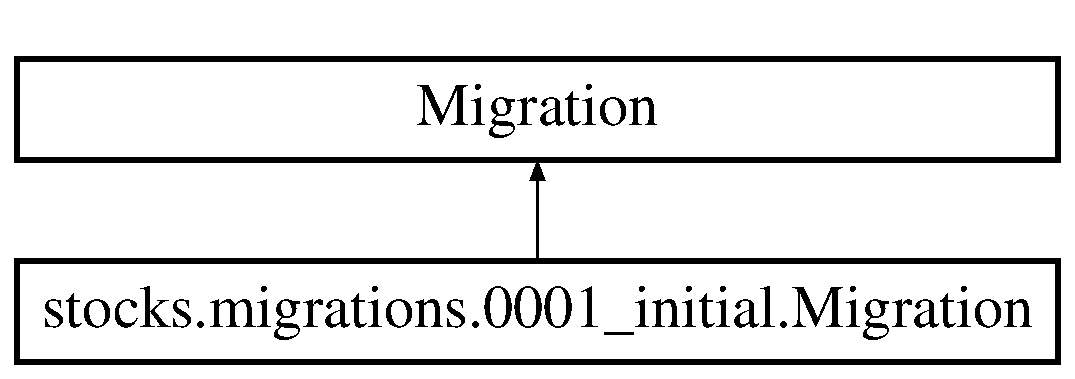
\includegraphics[height=2.000000cm]{classstocks_1_1migrations_1_10001__initial_1_1_migration}
\end{center}
\end{figure}
\subsection*{Static Public Attributes}
\begin{DoxyCompactItemize}
\item 
\mbox{\Hypertarget{classstocks_1_1migrations_1_10001__initial_1_1_migration_afc1023a8bab2daff2911fe5db9cba6aa}\label{classstocks_1_1migrations_1_10001__initial_1_1_migration_afc1023a8bab2daff2911fe5db9cba6aa}} 
bool {\bfseries initial} = True
\item 
list {\bfseries dependencies}
\item 
list {\bfseries operations}
\end{DoxyCompactItemize}


\subsection{Member Data Documentation}
\mbox{\Hypertarget{classstocks_1_1migrations_1_10001__initial_1_1_migration_a816085cec6cdb4a96f07c835b9dc5c1e}\label{classstocks_1_1migrations_1_10001__initial_1_1_migration_a816085cec6cdb4a96f07c835b9dc5c1e}} 
\index{stocks\+::migrations\+::0001\+\_\+initial\+::\+Migration@{stocks\+::migrations\+::0001\+\_\+initial\+::\+Migration}!dependencies@{dependencies}}
\index{dependencies@{dependencies}!stocks\+::migrations\+::0001\+\_\+initial\+::\+Migration@{stocks\+::migrations\+::0001\+\_\+initial\+::\+Migration}}
\subsubsection{\texorpdfstring{dependencies}{dependencies}}
{\footnotesize\ttfamily list stocks.\+migrations.\+0001\+\_\+initial.\+Migration.\+dependencies\hspace{0.3cm}{\ttfamily [static]}}

{\bfseries Initial value\+:}
\begin{DoxyCode}
=  [
    ]
\end{DoxyCode}
\mbox{\Hypertarget{classstocks_1_1migrations_1_10001__initial_1_1_migration_ad7876765d8e1c6ddc79df3f27a4e6901}\label{classstocks_1_1migrations_1_10001__initial_1_1_migration_ad7876765d8e1c6ddc79df3f27a4e6901}} 
\index{stocks\+::migrations\+::0001\+\_\+initial\+::\+Migration@{stocks\+::migrations\+::0001\+\_\+initial\+::\+Migration}!operations@{operations}}
\index{operations@{operations}!stocks\+::migrations\+::0001\+\_\+initial\+::\+Migration@{stocks\+::migrations\+::0001\+\_\+initial\+::\+Migration}}
\subsubsection{\texorpdfstring{operations}{operations}}
{\footnotesize\ttfamily list stocks.\+migrations.\+0001\+\_\+initial.\+Migration.\+operations\hspace{0.3cm}{\ttfamily [static]}}

{\bfseries Initial value\+:}
\begin{DoxyCode}
=  [
        migrations.CreateModel(
            name=\textcolor{stringliteral}{'Stock'},
            fields=[
                (\textcolor{stringliteral}{'id'}, models.AutoField(auto\_created=\textcolor{keyword}{True}, primary\_key=\textcolor{keyword}{True}, serialize=\textcolor{keyword}{False}, verbose\_name=\textcolor{stringliteral}{
      'ID'})),
                (\textcolor{stringliteral}{'ticker'}, models.CharField(max\_length=50)),
                (\textcolor{stringliteral}{'high'}, models.FloatField(blank=\textcolor{keyword}{True}, default=0)),
                (\textcolor{stringliteral}{'low'}, models.FloatField(blank=\textcolor{keyword}{True}, default=0)),
                (\textcolor{stringliteral}{'opening'}, models.FloatField(blank=\textcolor{keyword}{True}, default=0)),
                (\textcolor{stringliteral}{'closing'}, models.FloatField(blank=\textcolor{keyword}{True}, default=0)),
                (\textcolor{stringliteral}{'volume'}, models.IntegerField(blank=\textcolor{keyword}{True}, default=0)),
                (\textcolor{stringliteral}{'date'}, models.DateField(blank=\textcolor{keyword}{True}, null=\textcolor{keyword}{True})),
            ],
        ),
    ]
\end{DoxyCode}


The documentation for this class was generated from the following file\+:\begin{DoxyCompactItemize}
\item 
backend/stocks/migrations/0001\+\_\+initial.\+py\end{DoxyCompactItemize}

\hypertarget{classdata__mine_1_1_mine_company_names_1_1_mine_company_names}{}\section{data\+\_\+mine.\+Mine\+Company\+Names.\+Mine\+Company\+Names Class Reference}
\label{classdata__mine_1_1_mine_company_names_1_1_mine_company_names}\index{data\+\_\+mine.\+Mine\+Company\+Names.\+Mine\+Company\+Names@{data\+\_\+mine.\+Mine\+Company\+Names.\+Mine\+Company\+Names}}
\subsection*{Public Member Functions}
\begin{DoxyCompactItemize}
\item 
\mbox{\Hypertarget{classdata__mine_1_1_mine_company_names_1_1_mine_company_names_a97f2a5d06a1cdeb94818272def03e6ad}\label{classdata__mine_1_1_mine_company_names_1_1_mine_company_names_a97f2a5d06a1cdeb94818272def03e6ad}} 
def {\bfseries \+\_\+\+\_\+init\+\_\+\+\_\+} (self)
\item 
\mbox{\Hypertarget{classdata__mine_1_1_mine_company_names_1_1_mine_company_names_a2dfa3d83f4ce40299b4daa5fd436865a}\label{classdata__mine_1_1_mine_company_names_1_1_mine_company_names_a2dfa3d83f4ce40299b4daa5fd436865a}} 
def {\bfseries find\+\_\+company\+\_\+names} (self, soup)
\item 
\mbox{\Hypertarget{classdata__mine_1_1_mine_company_names_1_1_mine_company_names_aba839cc008e97f6275cfe189b907dc79}\label{classdata__mine_1_1_mine_company_names_1_1_mine_company_names_aba839cc008e97f6275cfe189b907dc79}} 
def {\bfseries post\+\_\+to\+\_\+api} (self, companies)
\item 
\mbox{\Hypertarget{classdata__mine_1_1_mine_company_names_1_1_mine_company_names_a8cb5cf8d03ad0cb7232fa605bc4f714e}\label{classdata__mine_1_1_mine_company_names_1_1_mine_company_names_a8cb5cf8d03ad0cb7232fa605bc4f714e}} 
def {\bfseries find\+\_\+urls} (self, soup)
\item 
\mbox{\Hypertarget{classdata__mine_1_1_mine_company_names_1_1_mine_company_names_a6f2a4b9f458f29df5041f9ed038b2c55}\label{classdata__mine_1_1_mine_company_names_1_1_mine_company_names_a6f2a4b9f458f29df5041f9ed038b2c55}} 
def {\bfseries get\+\_\+soup} (self, url)
\item 
\mbox{\Hypertarget{classdata__mine_1_1_mine_company_names_1_1_mine_company_names_a8bbd851be671d9eb982bec2d61ee9258}\label{classdata__mine_1_1_mine_company_names_1_1_mine_company_names_a8bbd851be671d9eb982bec2d61ee9258}} 
def {\bfseries run} (self)
\end{DoxyCompactItemize}
\subsection*{Public Attributes}
\begin{DoxyCompactItemize}
\item 
\mbox{\Hypertarget{classdata__mine_1_1_mine_company_names_1_1_mine_company_names_ab9f679172eb7fa5a318b7d369b6b0c31}\label{classdata__mine_1_1_mine_company_names_1_1_mine_company_names_ab9f679172eb7fa5a318b7d369b6b0c31}} 
{\bfseries http}
\item 
\mbox{\Hypertarget{classdata__mine_1_1_mine_company_names_1_1_mine_company_names_a8d68b3612e15050e8e95ae38532013e7}\label{classdata__mine_1_1_mine_company_names_1_1_mine_company_names_a8d68b3612e15050e8e95ae38532013e7}} 
{\bfseries base}
\item 
\mbox{\Hypertarget{classdata__mine_1_1_mine_company_names_1_1_mine_company_names_a496516ceb33d6d4c1bfc9df6c4f6e1f7}\label{classdata__mine_1_1_mine_company_names_1_1_mine_company_names_a496516ceb33d6d4c1bfc9df6c4f6e1f7}} 
{\bfseries website}
\item 
\mbox{\Hypertarget{classdata__mine_1_1_mine_company_names_1_1_mine_company_names_a55fdcedd272960dcd39e1edb87a06686}\label{classdata__mine_1_1_mine_company_names_1_1_mine_company_names_a55fdcedd272960dcd39e1edb87a06686}} 
{\bfseries api}
\item 
\mbox{\Hypertarget{classdata__mine_1_1_mine_company_names_1_1_mine_company_names_a68055c64a3c1472b02c29818389fe18f}\label{classdata__mine_1_1_mine_company_names_1_1_mine_company_names_a68055c64a3c1472b02c29818389fe18f}} 
{\bfseries links}
\item 
\mbox{\Hypertarget{classdata__mine_1_1_mine_company_names_1_1_mine_company_names_a59c673078f28bb0ef69265b0f2414288}\label{classdata__mine_1_1_mine_company_names_1_1_mine_company_names_a59c673078f28bb0ef69265b0f2414288}} 
{\bfseries soups}
\end{DoxyCompactItemize}


The documentation for this class was generated from the following file\+:\begin{DoxyCompactItemize}
\item 
backend/data\+\_\+mine/Mine\+Company\+Names.\+py\end{DoxyCompactItemize}

\hypertarget{classdata__mine_1_1tests_1_1test__mine_company_names_1_1_mine_company_names_test_case}{}\section{data\+\_\+mine.\+tests.\+test\+\_\+mine\+Company\+Names.\+Mine\+Company\+Names\+Test\+Case Class Reference}
\label{classdata__mine_1_1tests_1_1test__mine_company_names_1_1_mine_company_names_test_case}\index{data\+\_\+mine.\+tests.\+test\+\_\+mine\+Company\+Names.\+Mine\+Company\+Names\+Test\+Case@{data\+\_\+mine.\+tests.\+test\+\_\+mine\+Company\+Names.\+Mine\+Company\+Names\+Test\+Case}}
Inheritance diagram for data\+\_\+mine.\+tests.\+test\+\_\+mine\+Company\+Names.\+Mine\+Company\+Names\+Test\+Case\+:\begin{figure}[H]
\begin{center}
\leavevmode
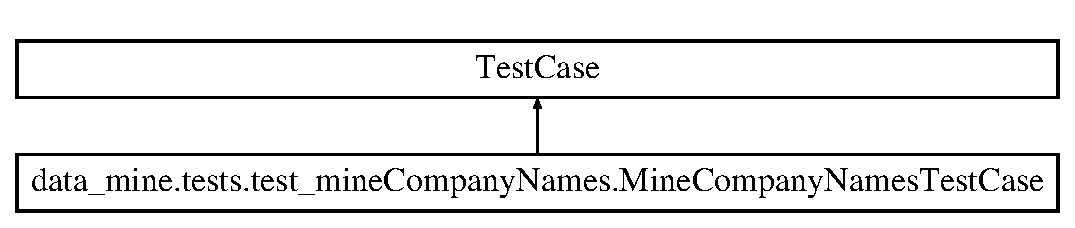
\includegraphics[height=2.000000cm]{classdata__mine_1_1tests_1_1test__mine_company_names_1_1_mine_company_names_test_case}
\end{center}
\end{figure}
\subsection*{Public Member Functions}
\begin{DoxyCompactItemize}
\item 
\mbox{\Hypertarget{classdata__mine_1_1tests_1_1test__mine_company_names_1_1_mine_company_names_test_case_a1d2e0811c2e6cec98e4a44bab307816e}\label{classdata__mine_1_1tests_1_1test__mine_company_names_1_1_mine_company_names_test_case_a1d2e0811c2e6cec98e4a44bab307816e}} 
def {\bfseries test\+\_\+post\+\_\+to\+\_\+api} (self)
\item 
\mbox{\Hypertarget{classdata__mine_1_1tests_1_1test__mine_company_names_1_1_mine_company_names_test_case_adbbbbf0c3370a4b298d0bd033ff52182}\label{classdata__mine_1_1tests_1_1test__mine_company_names_1_1_mine_company_names_test_case_adbbbbf0c3370a4b298d0bd033ff52182}} 
def {\bfseries tear\+Down} (self)
\end{DoxyCompactItemize}
\subsection*{Static Public Attributes}
\begin{DoxyCompactItemize}
\item 
\mbox{\Hypertarget{classdata__mine_1_1tests_1_1test__mine_company_names_1_1_mine_company_names_test_case_acbac6b97ebcbd6e04536ba7049e0d236}\label{classdata__mine_1_1tests_1_1test__mine_company_names_1_1_mine_company_names_test_case_acbac6b97ebcbd6e04536ba7049e0d236}} 
string {\bfseries pdg\+\_\+link} = \textquotesingle{}http\+://prodigal-\/ml.\+us-\/east-\/2.elasticbeanstalk.\+com/companies/\textquotesingle{}
\item 
\mbox{\Hypertarget{classdata__mine_1_1tests_1_1test__mine_company_names_1_1_mine_company_names_test_case_aee3a811aa5a0f812b366fc0a908fe439}\label{classdata__mine_1_1tests_1_1test__mine_company_names_1_1_mine_company_names_test_case_aee3a811aa5a0f812b366fc0a908fe439}} 
{\bfseries mcn} = \mbox{\hyperlink{classdata__mine_1_1_mine_company_names_1_1_mine_company_names}{Mine\+Company\+Names}}()
\end{DoxyCompactItemize}


The documentation for this class was generated from the following file\+:\begin{DoxyCompactItemize}
\item 
backend/data\+\_\+mine/tests/test\+\_\+mine\+Company\+Names.\+py\end{DoxyCompactItemize}

\hypertarget{classdata__mine_1_1_mine_stock_prices_1_1_mine_stock_prices}{}\section{data\+\_\+mine.\+Mine\+Stock\+Prices.\+Mine\+Stock\+Prices Class Reference}
\label{classdata__mine_1_1_mine_stock_prices_1_1_mine_stock_prices}\index{data\+\_\+mine.\+Mine\+Stock\+Prices.\+Mine\+Stock\+Prices@{data\+\_\+mine.\+Mine\+Stock\+Prices.\+Mine\+Stock\+Prices}}
\subsection*{Public Member Functions}
\begin{DoxyCompactItemize}
\item 
def \mbox{\hyperlink{classdata__mine_1_1_mine_stock_prices_1_1_mine_stock_prices_a9451b88181645b907f525b9ed63f65b0}{\+\_\+\+\_\+init\+\_\+\+\_\+}} (self)
\item 
def \mbox{\hyperlink{classdata__mine_1_1_mine_stock_prices_1_1_mine_stock_prices_a079e6738aef24fb09b5c23a1b97e97f4}{get\+\_\+response\+\_\+from\+\_\+api}} (self, function, search\+\_\+term, datatype=\char`\"{}json\char`\"{}, interval=None)
\item 
def \mbox{\hyperlink{classdata__mine_1_1_mine_stock_prices_1_1_mine_stock_prices_a9b73eb16d981aa9ebb8f2bdfbd3084cc}{get\+\_\+intraday\+\_\+stocks}} (self, search\+\_\+term, interval=\char`\"{}15min\char`\"{})
\item 
def \mbox{\hyperlink{classdata__mine_1_1_mine_stock_prices_1_1_mine_stock_prices_a4b892c0fb91e6bfd57e58bd0afae29f0}{get\+\_\+daily\+\_\+stocks}} (self, search\+\_\+term)
\item 
def \mbox{\hyperlink{classdata__mine_1_1_mine_stock_prices_1_1_mine_stock_prices_a98f05c73f0e1d30d16d42eb7510d60de}{get\+\_\+weekly\+\_\+stocks}} (self, search\+\_\+term, datatype)
\item 
def \mbox{\hyperlink{classdata__mine_1_1_mine_stock_prices_1_1_mine_stock_prices_a4e1c7514206e1ea659893e630a3e3ce7}{get\+\_\+monthly\+\_\+stocks}} (self, search\+\_\+term)
\item 
\mbox{\Hypertarget{classdata__mine_1_1_mine_stock_prices_1_1_mine_stock_prices_a6ed118f8260ea93e1c4667f725b53855}\label{classdata__mine_1_1_mine_stock_prices_1_1_mine_stock_prices_a6ed118f8260ea93e1c4667f725b53855}} 
def {\bfseries get\+\_\+intraday\+\_\+cryptos} (self)
\item 
\mbox{\Hypertarget{classdata__mine_1_1_mine_stock_prices_1_1_mine_stock_prices_a11108962a4b8b0c1853d4887e9d0d485}\label{classdata__mine_1_1_mine_stock_prices_1_1_mine_stock_prices_a11108962a4b8b0c1853d4887e9d0d485}} 
def {\bfseries get\+\_\+daily\+\_\+cryptos} (self)
\item 
\mbox{\Hypertarget{classdata__mine_1_1_mine_stock_prices_1_1_mine_stock_prices_a4c344c50b861530252a3dd75a27696c1}\label{classdata__mine_1_1_mine_stock_prices_1_1_mine_stock_prices_a4c344c50b861530252a3dd75a27696c1}} 
def {\bfseries get\+\_\+weekly\+\_\+cryptos} (self)
\item 
\mbox{\Hypertarget{classdata__mine_1_1_mine_stock_prices_1_1_mine_stock_prices_ab766380a3f24e5adfe8127fd2a3be6a0}\label{classdata__mine_1_1_mine_stock_prices_1_1_mine_stock_prices_ab766380a3f24e5adfe8127fd2a3be6a0}} 
def {\bfseries get\+\_\+monthly\+\_\+cryptos} (self)
\item 
\mbox{\Hypertarget{classdata__mine_1_1_mine_stock_prices_1_1_mine_stock_prices_a9639ea8ba431172f48d3065455a32193}\label{classdata__mine_1_1_mine_stock_prices_1_1_mine_stock_prices_a9639ea8ba431172f48d3065455a32193}} 
def {\bfseries write\+\_\+each\+\_\+ticker\+\_\+to\+\_\+file} (self)
\end{DoxyCompactItemize}


\subsection{Detailed Description}
\begin{DoxyVerb}    MineStockPrices is the class used to pull stock prices data from API.
    Currently using alphavantage.co API to pull data.
    Supports intraday, daily, weekly and monthly prices of tickers.
    Can extend into cryptocurrencies in the future.
\end{DoxyVerb}
 

\subsection{Constructor \& Destructor Documentation}
\mbox{\Hypertarget{classdata__mine_1_1_mine_stock_prices_1_1_mine_stock_prices_a9451b88181645b907f525b9ed63f65b0}\label{classdata__mine_1_1_mine_stock_prices_1_1_mine_stock_prices_a9451b88181645b907f525b9ed63f65b0}} 
\index{data\+\_\+mine\+::\+Mine\+Stock\+Prices\+::\+Mine\+Stock\+Prices@{data\+\_\+mine\+::\+Mine\+Stock\+Prices\+::\+Mine\+Stock\+Prices}!\+\_\+\+\_\+init\+\_\+\+\_\+@{\+\_\+\+\_\+init\+\_\+\+\_\+}}
\index{\+\_\+\+\_\+init\+\_\+\+\_\+@{\+\_\+\+\_\+init\+\_\+\+\_\+}!data\+\_\+mine\+::\+Mine\+Stock\+Prices\+::\+Mine\+Stock\+Prices@{data\+\_\+mine\+::\+Mine\+Stock\+Prices\+::\+Mine\+Stock\+Prices}}
\subsubsection{\texorpdfstring{\+\_\+\+\_\+init\+\_\+\+\_\+()}{\_\_init\_\_()}}
{\footnotesize\ttfamily def data\+\_\+mine.\+Mine\+Stock\+Prices.\+Mine\+Stock\+Prices.\+\_\+\+\_\+init\+\_\+\+\_\+ (\begin{DoxyParamCaption}\item[{}]{self }\end{DoxyParamCaption})}

\begin{DoxyVerb}    Constructor for MineStockPrices.
    Initializes two instance variables.
    _api_key: API token for alphavantage.co
    _base_url: Base URL to call alaphavantage API
\end{DoxyVerb}
 

\subsection{Member Function Documentation}
\mbox{\Hypertarget{classdata__mine_1_1_mine_stock_prices_1_1_mine_stock_prices_a4b892c0fb91e6bfd57e58bd0afae29f0}\label{classdata__mine_1_1_mine_stock_prices_1_1_mine_stock_prices_a4b892c0fb91e6bfd57e58bd0afae29f0}} 
\index{data\+\_\+mine\+::\+Mine\+Stock\+Prices\+::\+Mine\+Stock\+Prices@{data\+\_\+mine\+::\+Mine\+Stock\+Prices\+::\+Mine\+Stock\+Prices}!get\+\_\+daily\+\_\+stocks@{get\+\_\+daily\+\_\+stocks}}
\index{get\+\_\+daily\+\_\+stocks@{get\+\_\+daily\+\_\+stocks}!data\+\_\+mine\+::\+Mine\+Stock\+Prices\+::\+Mine\+Stock\+Prices@{data\+\_\+mine\+::\+Mine\+Stock\+Prices\+::\+Mine\+Stock\+Prices}}
\subsubsection{\texorpdfstring{get\+\_\+daily\+\_\+stocks()}{get\_daily\_stocks()}}
{\footnotesize\ttfamily def data\+\_\+mine.\+Mine\+Stock\+Prices.\+Mine\+Stock\+Prices.\+get\+\_\+daily\+\_\+stocks (\begin{DoxyParamCaption}\item[{}]{self,  }\item[{}]{search\+\_\+term }\end{DoxyParamCaption})}

\begin{DoxyVerb}    Get stock prices of a company daily.
    Default number of entries returned is latest 100 data points.
    Default return format is JSON.
    search_term: ticker symbol to search for stock prices
\end{DoxyVerb}
 \mbox{\Hypertarget{classdata__mine_1_1_mine_stock_prices_1_1_mine_stock_prices_a9b73eb16d981aa9ebb8f2bdfbd3084cc}\label{classdata__mine_1_1_mine_stock_prices_1_1_mine_stock_prices_a9b73eb16d981aa9ebb8f2bdfbd3084cc}} 
\index{data\+\_\+mine\+::\+Mine\+Stock\+Prices\+::\+Mine\+Stock\+Prices@{data\+\_\+mine\+::\+Mine\+Stock\+Prices\+::\+Mine\+Stock\+Prices}!get\+\_\+intraday\+\_\+stocks@{get\+\_\+intraday\+\_\+stocks}}
\index{get\+\_\+intraday\+\_\+stocks@{get\+\_\+intraday\+\_\+stocks}!data\+\_\+mine\+::\+Mine\+Stock\+Prices\+::\+Mine\+Stock\+Prices@{data\+\_\+mine\+::\+Mine\+Stock\+Prices\+::\+Mine\+Stock\+Prices}}
\subsubsection{\texorpdfstring{get\+\_\+intraday\+\_\+stocks()}{get\_intraday\_stocks()}}
{\footnotesize\ttfamily def data\+\_\+mine.\+Mine\+Stock\+Prices.\+Mine\+Stock\+Prices.\+get\+\_\+intraday\+\_\+stocks (\begin{DoxyParamCaption}\item[{}]{self,  }\item[{}]{search\+\_\+term,  }\item[{}]{interval = {\ttfamily \char`\"{}15min\char`\"{}} }\end{DoxyParamCaption})}

\begin{DoxyVerb}    Get stock prices of a paricular company within one day.
    Default time interval between each API pull is 15 minutes.
    Default return format is JSON.
    search_term: ticker symbol to search for stock prices
\end{DoxyVerb}
 \mbox{\Hypertarget{classdata__mine_1_1_mine_stock_prices_1_1_mine_stock_prices_a4e1c7514206e1ea659893e630a3e3ce7}\label{classdata__mine_1_1_mine_stock_prices_1_1_mine_stock_prices_a4e1c7514206e1ea659893e630a3e3ce7}} 
\index{data\+\_\+mine\+::\+Mine\+Stock\+Prices\+::\+Mine\+Stock\+Prices@{data\+\_\+mine\+::\+Mine\+Stock\+Prices\+::\+Mine\+Stock\+Prices}!get\+\_\+monthly\+\_\+stocks@{get\+\_\+monthly\+\_\+stocks}}
\index{get\+\_\+monthly\+\_\+stocks@{get\+\_\+monthly\+\_\+stocks}!data\+\_\+mine\+::\+Mine\+Stock\+Prices\+::\+Mine\+Stock\+Prices@{data\+\_\+mine\+::\+Mine\+Stock\+Prices\+::\+Mine\+Stock\+Prices}}
\subsubsection{\texorpdfstring{get\+\_\+monthly\+\_\+stocks()}{get\_monthly\_stocks()}}
{\footnotesize\ttfamily def data\+\_\+mine.\+Mine\+Stock\+Prices.\+Mine\+Stock\+Prices.\+get\+\_\+monthly\+\_\+stocks (\begin{DoxyParamCaption}\item[{}]{self,  }\item[{}]{search\+\_\+term }\end{DoxyParamCaption})}

\begin{DoxyVerb}    Get stock prices of a company monthly.
    Default number of entries returned is latest 100 data points.
    Default return format is JSON.
    search_term: ticker symbol to search for stock prices
\end{DoxyVerb}
 \mbox{\Hypertarget{classdata__mine_1_1_mine_stock_prices_1_1_mine_stock_prices_a079e6738aef24fb09b5c23a1b97e97f4}\label{classdata__mine_1_1_mine_stock_prices_1_1_mine_stock_prices_a079e6738aef24fb09b5c23a1b97e97f4}} 
\index{data\+\_\+mine\+::\+Mine\+Stock\+Prices\+::\+Mine\+Stock\+Prices@{data\+\_\+mine\+::\+Mine\+Stock\+Prices\+::\+Mine\+Stock\+Prices}!get\+\_\+response\+\_\+from\+\_\+api@{get\+\_\+response\+\_\+from\+\_\+api}}
\index{get\+\_\+response\+\_\+from\+\_\+api@{get\+\_\+response\+\_\+from\+\_\+api}!data\+\_\+mine\+::\+Mine\+Stock\+Prices\+::\+Mine\+Stock\+Prices@{data\+\_\+mine\+::\+Mine\+Stock\+Prices\+::\+Mine\+Stock\+Prices}}
\subsubsection{\texorpdfstring{get\+\_\+response\+\_\+from\+\_\+api()}{get\_response\_from\_api()}}
{\footnotesize\ttfamily def data\+\_\+mine.\+Mine\+Stock\+Prices.\+Mine\+Stock\+Prices.\+get\+\_\+response\+\_\+from\+\_\+api (\begin{DoxyParamCaption}\item[{}]{self,  }\item[{}]{function,  }\item[{}]{search\+\_\+term,  }\item[{}]{datatype = {\ttfamily \char`\"{}json\char`\"{}},  }\item[{}]{interval = {\ttfamily None} }\end{DoxyParamCaption})}

\begin{DoxyVerb}    Helper method to return json objects of ticker symbol from API
    function: table/database name defined by alphavantage.co
    search_term: ticker symbol to search for stock prices
\end{DoxyVerb}
 \mbox{\Hypertarget{classdata__mine_1_1_mine_stock_prices_1_1_mine_stock_prices_a98f05c73f0e1d30d16d42eb7510d60de}\label{classdata__mine_1_1_mine_stock_prices_1_1_mine_stock_prices_a98f05c73f0e1d30d16d42eb7510d60de}} 
\index{data\+\_\+mine\+::\+Mine\+Stock\+Prices\+::\+Mine\+Stock\+Prices@{data\+\_\+mine\+::\+Mine\+Stock\+Prices\+::\+Mine\+Stock\+Prices}!get\+\_\+weekly\+\_\+stocks@{get\+\_\+weekly\+\_\+stocks}}
\index{get\+\_\+weekly\+\_\+stocks@{get\+\_\+weekly\+\_\+stocks}!data\+\_\+mine\+::\+Mine\+Stock\+Prices\+::\+Mine\+Stock\+Prices@{data\+\_\+mine\+::\+Mine\+Stock\+Prices\+::\+Mine\+Stock\+Prices}}
\subsubsection{\texorpdfstring{get\+\_\+weekly\+\_\+stocks()}{get\_weekly\_stocks()}}
{\footnotesize\ttfamily def data\+\_\+mine.\+Mine\+Stock\+Prices.\+Mine\+Stock\+Prices.\+get\+\_\+weekly\+\_\+stocks (\begin{DoxyParamCaption}\item[{}]{self,  }\item[{}]{search\+\_\+term,  }\item[{}]{datatype }\end{DoxyParamCaption})}

\begin{DoxyVerb}    Get stock prices of a company weekly.
    Default number of entries returned is latest 100 data points.
    Default return format is JSON.
    search_term: ticker symbol to search for stock prices
\end{DoxyVerb}
 

The documentation for this class was generated from the following file\+:\begin{DoxyCompactItemize}
\item 
backend/data\+\_\+mine/Mine\+Stock\+Prices.\+py\end{DoxyCompactItemize}

\hypertarget{classdata__mine_1_1tests_1_1test___mine_stock_prices_1_1_mine_stock_prices_test_case}{}\section{data\+\_\+mine.\+tests.\+test\+\_\+\+Mine\+Stock\+Prices.\+Mine\+Stock\+Prices\+Test\+Case Class Reference}
\label{classdata__mine_1_1tests_1_1test___mine_stock_prices_1_1_mine_stock_prices_test_case}\index{data\+\_\+mine.\+tests.\+test\+\_\+\+Mine\+Stock\+Prices.\+Mine\+Stock\+Prices\+Test\+Case@{data\+\_\+mine.\+tests.\+test\+\_\+\+Mine\+Stock\+Prices.\+Mine\+Stock\+Prices\+Test\+Case}}
Inheritance diagram for data\+\_\+mine.\+tests.\+test\+\_\+\+Mine\+Stock\+Prices.\+Mine\+Stock\+Prices\+Test\+Case\+:\begin{figure}[H]
\begin{center}
\leavevmode
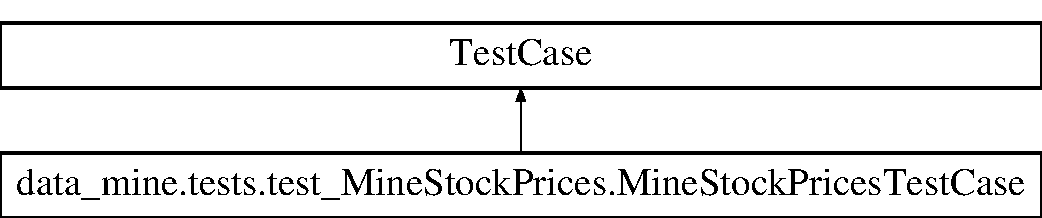
\includegraphics[height=2.000000cm]{classdata__mine_1_1tests_1_1test___mine_stock_prices_1_1_mine_stock_prices_test_case}
\end{center}
\end{figure}
\subsection*{Public Member Functions}
\begin{DoxyCompactItemize}
\item 
\mbox{\Hypertarget{classdata__mine_1_1tests_1_1test___mine_stock_prices_1_1_mine_stock_prices_test_case_aaa403c5596d49b7b948b182b6a626b07}\label{classdata__mine_1_1tests_1_1test___mine_stock_prices_1_1_mine_stock_prices_test_case_aaa403c5596d49b7b948b182b6a626b07}} 
def {\bfseries test\+\_\+get\+\_\+daily\+\_\+stocks} (self)
\end{DoxyCompactItemize}
\subsection*{Static Public Attributes}
\begin{DoxyCompactItemize}
\item 
\mbox{\Hypertarget{classdata__mine_1_1tests_1_1test___mine_stock_prices_1_1_mine_stock_prices_test_case_a11bf496d00111a6b5f043452294d27cb}\label{classdata__mine_1_1tests_1_1test___mine_stock_prices_1_1_mine_stock_prices_test_case_a11bf496d00111a6b5f043452294d27cb}} 
string {\bfseries pdg\+\_\+link} = \textquotesingle{}http\+://prodigal-\/ml.\+us-\/east-\/2.elasticbeanstalk.\+com/stocks/\textquotesingle{}
\item 
\mbox{\Hypertarget{classdata__mine_1_1tests_1_1test___mine_stock_prices_1_1_mine_stock_prices_test_case_abddea13e780cdd2836b5834e8ddc96ba}\label{classdata__mine_1_1tests_1_1test___mine_stock_prices_1_1_mine_stock_prices_test_case_abddea13e780cdd2836b5834e8ddc96ba}} 
{\bfseries msp} = \mbox{\hyperlink{classdata__mine_1_1_mine_stock_prices_1_1_mine_stock_prices}{Mine\+Stock\+Prices}}()
\end{DoxyCompactItemize}


The documentation for this class was generated from the following file\+:\begin{DoxyCompactItemize}
\item 
backend/data\+\_\+mine/tests/test\+\_\+\+Mine\+Stock\+Prices.\+py\end{DoxyCompactItemize}

\hypertarget{classdata__mine_1_1tests_1_1test__prediction_1_1_prediction_test_case}{}\section{data\+\_\+mine.\+tests.\+test\+\_\+prediction.\+Prediction\+Test\+Case Class Reference}
\label{classdata__mine_1_1tests_1_1test__prediction_1_1_prediction_test_case}\index{data\+\_\+mine.\+tests.\+test\+\_\+prediction.\+Prediction\+Test\+Case@{data\+\_\+mine.\+tests.\+test\+\_\+prediction.\+Prediction\+Test\+Case}}
Inheritance diagram for data\+\_\+mine.\+tests.\+test\+\_\+prediction.\+Prediction\+Test\+Case\+:\begin{figure}[H]
\begin{center}
\leavevmode
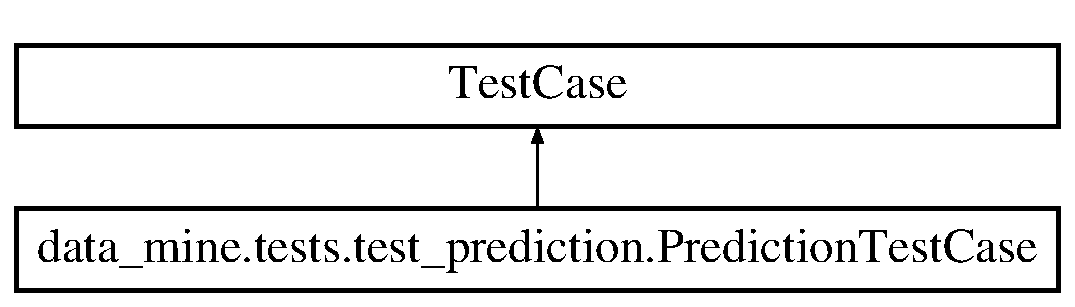
\includegraphics[height=2.000000cm]{classdata__mine_1_1tests_1_1test__prediction_1_1_prediction_test_case}
\end{center}
\end{figure}
\subsection*{Public Member Functions}
\begin{DoxyCompactItemize}
\item 
\mbox{\Hypertarget{classdata__mine_1_1tests_1_1test__prediction_1_1_prediction_test_case_a2e5006a91ee460cb1377c9cc676bd9bb}\label{classdata__mine_1_1tests_1_1test__prediction_1_1_prediction_test_case_a2e5006a91ee460cb1377c9cc676bd9bb}} 
def {\bfseries set\+Up\+Test\+Data} (self)
\item 
\mbox{\Hypertarget{classdata__mine_1_1tests_1_1test__prediction_1_1_prediction_test_case_abdfa5c1feb683aea3b67d15364770b5f}\label{classdata__mine_1_1tests_1_1test__prediction_1_1_prediction_test_case_abdfa5c1feb683aea3b67d15364770b5f}} 
def {\bfseries test\+\_\+prediction\+\_\+create} (self)
\end{DoxyCompactItemize}


The documentation for this class was generated from the following file\+:\begin{DoxyCompactItemize}
\item 
backend/data\+\_\+mine/tests/test\+\_\+prediction.\+py\end{DoxyCompactItemize}

\hypertarget{classstocks_1_1linear__regression_1_1_predictor}{}\section{stocks.\+linear\+\_\+regression.\+Predictor Class Reference}
\label{classstocks_1_1linear__regression_1_1_predictor}\index{stocks.\+linear\+\_\+regression.\+Predictor@{stocks.\+linear\+\_\+regression.\+Predictor}}
\subsection*{Public Member Functions}
\begin{DoxyCompactItemize}
\item 
def \mbox{\hyperlink{classstocks_1_1linear__regression_1_1_predictor_a87e63495df1ef8625b2321852477c34c}{return\+\_\+prediction}} (self, ticker\+\_\+symbol)
\end{DoxyCompactItemize}
\subsection*{Static Public Member Functions}
\begin{DoxyCompactItemize}
\item 
def \mbox{\hyperlink{classstocks_1_1linear__regression_1_1_predictor_a828b522dbfc376cb06d5e28a9baf3035}{get\+\_\+json}} (ticker\+\_\+symbol)
\item 
def \mbox{\hyperlink{classstocks_1_1linear__regression_1_1_predictor_aeee6845991ab04f14ce6a0541d7b2c6e}{create\+\_\+csv}} (json\+\_\+file)
\item 
def \mbox{\hyperlink{classstocks_1_1linear__regression_1_1_predictor_a5cd7db298bf453a953032e1458b5d17f}{predict\+\_\+closing}} (open\+\_\+price, high\+\_\+price, low\+\_\+price)
\end{DoxyCompactItemize}


\subsection{Detailed Description}
\begin{DoxyVerb}Class to run linear regression experiment and predict closing value from
given data of open, close, high, low and volume.
\end{DoxyVerb}
 

\subsection{Member Function Documentation}
\mbox{\Hypertarget{classstocks_1_1linear__regression_1_1_predictor_aeee6845991ab04f14ce6a0541d7b2c6e}\label{classstocks_1_1linear__regression_1_1_predictor_aeee6845991ab04f14ce6a0541d7b2c6e}} 
\index{stocks\+::linear\+\_\+regression\+::\+Predictor@{stocks\+::linear\+\_\+regression\+::\+Predictor}!create\+\_\+csv@{create\+\_\+csv}}
\index{create\+\_\+csv@{create\+\_\+csv}!stocks\+::linear\+\_\+regression\+::\+Predictor@{stocks\+::linear\+\_\+regression\+::\+Predictor}}
\subsubsection{\texorpdfstring{create\+\_\+csv()}{create\_csv()}}
{\footnotesize\ttfamily def stocks.\+linear\+\_\+regression.\+Predictor.\+create\+\_\+csv (\begin{DoxyParamCaption}\item[{}]{json\+\_\+file }\end{DoxyParamCaption})\hspace{0.3cm}{\ttfamily [static]}}

\begin{DoxyVerb}Creates csv file to feed in to prediction model from given JSON file
object.
:param json_file: JSON file object from get_json function.
:return: No return value.
\end{DoxyVerb}
 \mbox{\Hypertarget{classstocks_1_1linear__regression_1_1_predictor_a828b522dbfc376cb06d5e28a9baf3035}\label{classstocks_1_1linear__regression_1_1_predictor_a828b522dbfc376cb06d5e28a9baf3035}} 
\index{stocks\+::linear\+\_\+regression\+::\+Predictor@{stocks\+::linear\+\_\+regression\+::\+Predictor}!get\+\_\+json@{get\+\_\+json}}
\index{get\+\_\+json@{get\+\_\+json}!stocks\+::linear\+\_\+regression\+::\+Predictor@{stocks\+::linear\+\_\+regression\+::\+Predictor}}
\subsubsection{\texorpdfstring{get\+\_\+json()}{get\_json()}}
{\footnotesize\ttfamily def stocks.\+linear\+\_\+regression.\+Predictor.\+get\+\_\+json (\begin{DoxyParamCaption}\item[{}]{ticker\+\_\+symbol }\end{DoxyParamCaption})\hspace{0.3cm}{\ttfamily [static]}}

\begin{DoxyVerb}Gets history data of given ticker from API and returns them in
JSON file object.
:param ticker_symbol: Ticker to get data
:return: list of JSON objects of history of given ticker
\end{DoxyVerb}
 \mbox{\Hypertarget{classstocks_1_1linear__regression_1_1_predictor_a5cd7db298bf453a953032e1458b5d17f}\label{classstocks_1_1linear__regression_1_1_predictor_a5cd7db298bf453a953032e1458b5d17f}} 
\index{stocks\+::linear\+\_\+regression\+::\+Predictor@{stocks\+::linear\+\_\+regression\+::\+Predictor}!predict\+\_\+closing@{predict\+\_\+closing}}
\index{predict\+\_\+closing@{predict\+\_\+closing}!stocks\+::linear\+\_\+regression\+::\+Predictor@{stocks\+::linear\+\_\+regression\+::\+Predictor}}
\subsubsection{\texorpdfstring{predict\+\_\+closing()}{predict\_closing()}}
{\footnotesize\ttfamily def stocks.\+linear\+\_\+regression.\+Predictor.\+predict\+\_\+closing (\begin{DoxyParamCaption}\item[{}]{open\+\_\+price,  }\item[{}]{high\+\_\+price,  }\item[{}]{low\+\_\+price }\end{DoxyParamCaption})\hspace{0.3cm}{\ttfamily [static]}}

\begin{DoxyVerb}Predicts closing value from previous open, high, low data using linear
regression model. 70% of history data is used for training,
30% for testing.
:param open_price: open value to be used on prediction
:param high_price: high value to be used on prediction
:param low_price: low value to be used on prediction
:return: prediction result for closing value.
\end{DoxyVerb}
 \mbox{\Hypertarget{classstocks_1_1linear__regression_1_1_predictor_a87e63495df1ef8625b2321852477c34c}\label{classstocks_1_1linear__regression_1_1_predictor_a87e63495df1ef8625b2321852477c34c}} 
\index{stocks\+::linear\+\_\+regression\+::\+Predictor@{stocks\+::linear\+\_\+regression\+::\+Predictor}!return\+\_\+prediction@{return\+\_\+prediction}}
\index{return\+\_\+prediction@{return\+\_\+prediction}!stocks\+::linear\+\_\+regression\+::\+Predictor@{stocks\+::linear\+\_\+regression\+::\+Predictor}}
\subsubsection{\texorpdfstring{return\+\_\+prediction()}{return\_prediction()}}
{\footnotesize\ttfamily def stocks.\+linear\+\_\+regression.\+Predictor.\+return\+\_\+prediction (\begin{DoxyParamCaption}\item[{}]{self,  }\item[{}]{ticker\+\_\+symbol }\end{DoxyParamCaption})}

\begin{DoxyVerb}Runs prediction model on given ticker 5 times recursively, and return
prediction results for next 5 days.
:param ticker_symbol: Ticker to run experiment on
:return: List of prediction results.
\end{DoxyVerb}
 

The documentation for this class was generated from the following file\+:\begin{DoxyCompactItemize}
\item 
backend/stocks/linear\+\_\+regression.\+py\end{DoxyCompactItemize}

\hypertarget{classsnippets_1_1models_1_1_snippet}{}\section{snippets.\+models.\+Snippet Class Reference}
\label{classsnippets_1_1models_1_1_snippet}\index{snippets.\+models.\+Snippet@{snippets.\+models.\+Snippet}}
Inheritance diagram for snippets.\+models.\+Snippet\+:\begin{figure}[H]
\begin{center}
\leavevmode
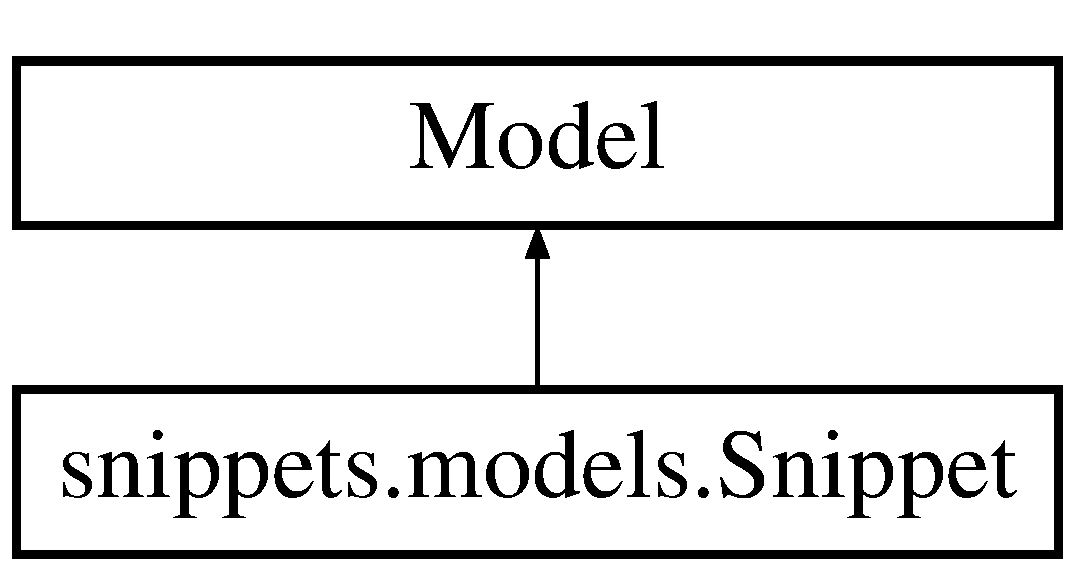
\includegraphics[height=2.000000cm]{classsnippets_1_1models_1_1_snippet}
\end{center}
\end{figure}
\subsection*{Classes}
\begin{DoxyCompactItemize}
\item 
class \mbox{\hyperlink{classsnippets_1_1models_1_1_snippet_1_1_meta}{Meta}}
\end{DoxyCompactItemize}
\subsection*{Static Public Attributes}
\begin{DoxyCompactItemize}
\item 
\mbox{\Hypertarget{classsnippets_1_1models_1_1_snippet_aedeb681049e2596085770c48f1af922a}\label{classsnippets_1_1models_1_1_snippet_aedeb681049e2596085770c48f1af922a}} 
{\bfseries created} = models.\+Date\+Time\+Field(auto\+\_\+now\+\_\+add=True)
\item 
\mbox{\Hypertarget{classsnippets_1_1models_1_1_snippet_a5bbd359692f190d321e36794640b117d}\label{classsnippets_1_1models_1_1_snippet_a5bbd359692f190d321e36794640b117d}} 
{\bfseries title} = models.\+Char\+Field(max\+\_\+length=100, blank=True, default=\textquotesingle{}\textquotesingle{})
\item 
\mbox{\Hypertarget{classsnippets_1_1models_1_1_snippet_ae1cb46d6f6321b5273615704befaaac1}\label{classsnippets_1_1models_1_1_snippet_ae1cb46d6f6321b5273615704befaaac1}} 
{\bfseries code} = models.\+Text\+Field()
\item 
\mbox{\Hypertarget{classsnippets_1_1models_1_1_snippet_aa8c07e2028d393a3589270f520eaedbc}\label{classsnippets_1_1models_1_1_snippet_aa8c07e2028d393a3589270f520eaedbc}} 
{\bfseries linenos} = models.\+Boolean\+Field(default=False)
\item 
\mbox{\Hypertarget{classsnippets_1_1models_1_1_snippet_af329e6de0796608bb90566efac1d9196}\label{classsnippets_1_1models_1_1_snippet_af329e6de0796608bb90566efac1d9196}} 
{\bfseries language} = models.\+Char\+Field(choices=L\+A\+N\+G\+U\+A\+G\+E\+\_\+\+C\+H\+O\+I\+C\+ES, default=\textquotesingle{}python\textquotesingle{}, max\+\_\+length=100)
\item 
\mbox{\Hypertarget{classsnippets_1_1models_1_1_snippet_aeb520e7dab031a04833cc0678822441e}\label{classsnippets_1_1models_1_1_snippet_aeb520e7dab031a04833cc0678822441e}} 
{\bfseries style} = models.\+Char\+Field(choices=S\+T\+Y\+L\+E\+\_\+\+C\+H\+O\+I\+C\+ES, default=\textquotesingle{}friendly\textquotesingle{}, max\+\_\+length=100)
\end{DoxyCompactItemize}


The documentation for this class was generated from the following file\+:\begin{DoxyCompactItemize}
\item 
spike/hwin16/mysite/snippets/models.\+py\end{DoxyCompactItemize}

\hypertarget{classsnippets_1_1views_1_1_snippet_detail}{}\section{snippets.\+views.\+Snippet\+Detail Class Reference}
\label{classsnippets_1_1views_1_1_snippet_detail}\index{snippets.\+views.\+Snippet\+Detail@{snippets.\+views.\+Snippet\+Detail}}
Inheritance diagram for snippets.\+views.\+Snippet\+Detail\+:\begin{figure}[H]
\begin{center}
\leavevmode
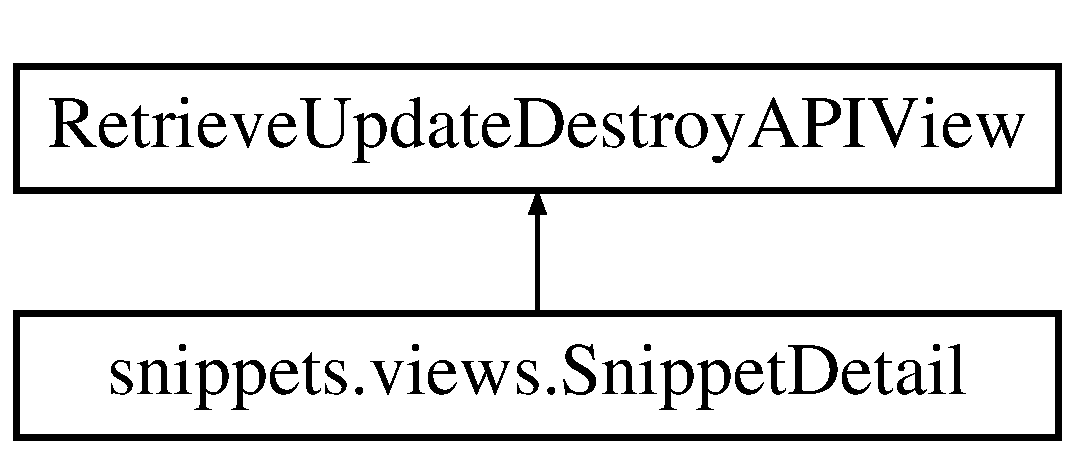
\includegraphics[height=2.000000cm]{classsnippets_1_1views_1_1_snippet_detail}
\end{center}
\end{figure}
\subsection*{Static Public Attributes}
\begin{DoxyCompactItemize}
\item 
\mbox{\Hypertarget{classsnippets_1_1views_1_1_snippet_detail_a9dfbcfb6881bf052630041ce0436d9cc}\label{classsnippets_1_1views_1_1_snippet_detail_a9dfbcfb6881bf052630041ce0436d9cc}} 
{\bfseries queryset} = Snippet.\+objects.\+all()
\item 
\mbox{\Hypertarget{classsnippets_1_1views_1_1_snippet_detail_aae643773a00409d96ce42878ed18d6f0}\label{classsnippets_1_1views_1_1_snippet_detail_aae643773a00409d96ce42878ed18d6f0}} 
{\bfseries serializer\+\_\+class} = \mbox{\hyperlink{classsnippets_1_1serializers_1_1_snippet_serializer}{Snippet\+Serializer}}
\end{DoxyCompactItemize}


The documentation for this class was generated from the following file\+:\begin{DoxyCompactItemize}
\item 
spike/hwin16/mysite/snippets/views.\+py\end{DoxyCompactItemize}

\hypertarget{classsnippets_1_1views_1_1_snippet_list}{}\section{snippets.\+views.\+Snippet\+List Class Reference}
\label{classsnippets_1_1views_1_1_snippet_list}\index{snippets.\+views.\+Snippet\+List@{snippets.\+views.\+Snippet\+List}}
Inheritance diagram for snippets.\+views.\+Snippet\+List\+:\begin{figure}[H]
\begin{center}
\leavevmode
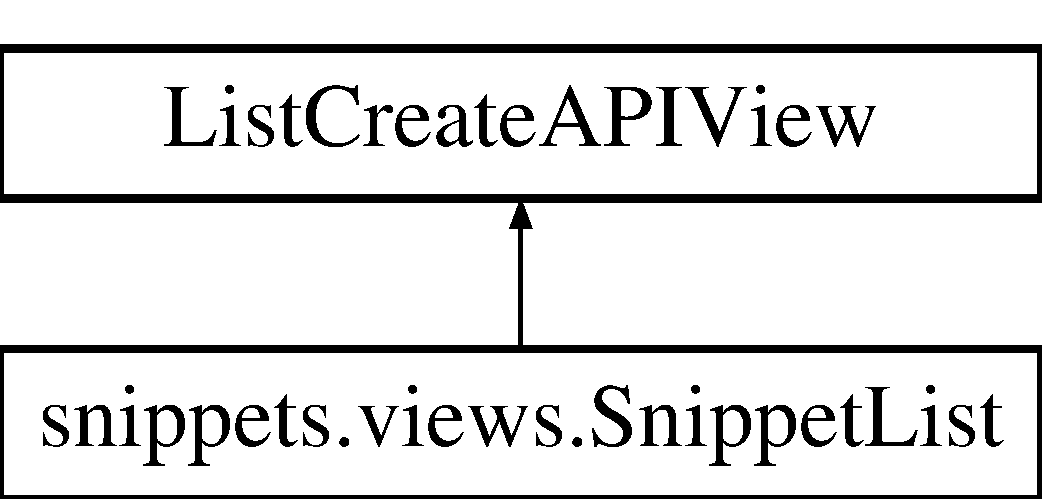
\includegraphics[height=2.000000cm]{classsnippets_1_1views_1_1_snippet_list}
\end{center}
\end{figure}
\subsection*{Static Public Attributes}
\begin{DoxyCompactItemize}
\item 
\mbox{\Hypertarget{classsnippets_1_1views_1_1_snippet_list_a368dca5c3168908e0d6cb96fee19f79a}\label{classsnippets_1_1views_1_1_snippet_list_a368dca5c3168908e0d6cb96fee19f79a}} 
{\bfseries queryset} = Snippet.\+objects.\+all()
\item 
\mbox{\Hypertarget{classsnippets_1_1views_1_1_snippet_list_a9dc5cbbc6d8e0143ef9c361d6d2f707e}\label{classsnippets_1_1views_1_1_snippet_list_a9dc5cbbc6d8e0143ef9c361d6d2f707e}} 
{\bfseries serializer\+\_\+class} = \mbox{\hyperlink{classsnippets_1_1serializers_1_1_snippet_serializer}{Snippet\+Serializer}}
\end{DoxyCompactItemize}


The documentation for this class was generated from the following file\+:\begin{DoxyCompactItemize}
\item 
spike/hwin16/mysite/snippets/views.\+py\end{DoxyCompactItemize}

\hypertarget{classsnippets_1_1apps_1_1_snippets_config}{}\section{snippets.\+apps.\+Snippets\+Config Class Reference}
\label{classsnippets_1_1apps_1_1_snippets_config}\index{snippets.\+apps.\+Snippets\+Config@{snippets.\+apps.\+Snippets\+Config}}
Inheritance diagram for snippets.\+apps.\+Snippets\+Config\+:\begin{figure}[H]
\begin{center}
\leavevmode
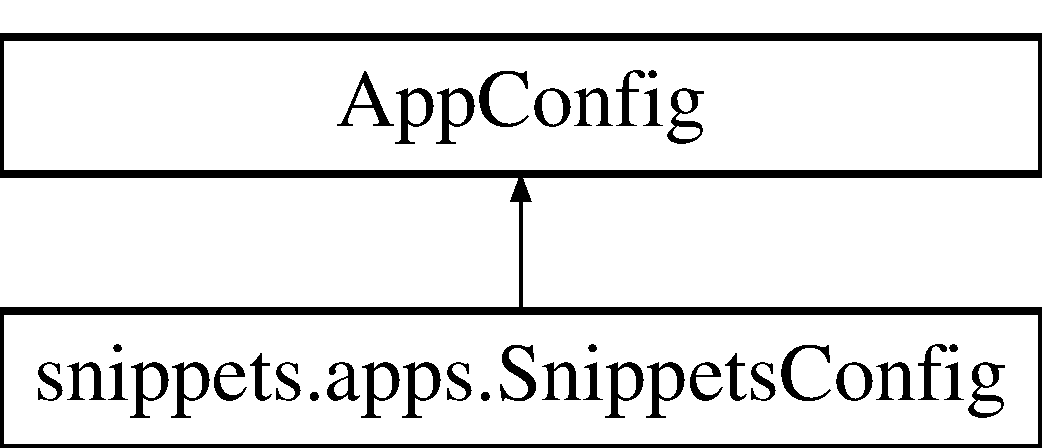
\includegraphics[height=2.000000cm]{classsnippets_1_1apps_1_1_snippets_config}
\end{center}
\end{figure}
\subsection*{Static Public Attributes}
\begin{DoxyCompactItemize}
\item 
\mbox{\Hypertarget{classsnippets_1_1apps_1_1_snippets_config_a78c4db1363915d3f9f12b28184eb8248}\label{classsnippets_1_1apps_1_1_snippets_config_a78c4db1363915d3f9f12b28184eb8248}} 
string {\bfseries name} = \textquotesingle{}snippets\textquotesingle{}
\end{DoxyCompactItemize}


The documentation for this class was generated from the following file\+:\begin{DoxyCompactItemize}
\item 
spike/hwin16/mysite/snippets/apps.\+py\end{DoxyCompactItemize}

\hypertarget{classsnippets_1_1serializers_1_1_snippet_serializer}{}\section{snippets.\+serializers.\+Snippet\+Serializer Class Reference}
\label{classsnippets_1_1serializers_1_1_snippet_serializer}\index{snippets.\+serializers.\+Snippet\+Serializer@{snippets.\+serializers.\+Snippet\+Serializer}}
Inheritance diagram for snippets.\+serializers.\+Snippet\+Serializer\+:\begin{figure}[H]
\begin{center}
\leavevmode
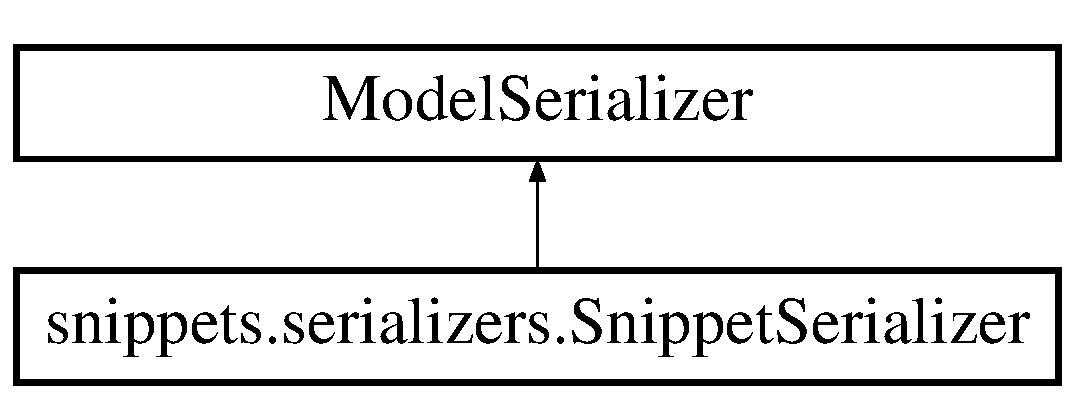
\includegraphics[height=2.000000cm]{classsnippets_1_1serializers_1_1_snippet_serializer}
\end{center}
\end{figure}
\subsection*{Classes}
\begin{DoxyCompactItemize}
\item 
class \mbox{\hyperlink{classsnippets_1_1serializers_1_1_snippet_serializer_1_1_meta}{Meta}}
\end{DoxyCompactItemize}


The documentation for this class was generated from the following file\+:\begin{DoxyCompactItemize}
\item 
spike/hwin16/mysite/snippets/serializers.\+py\end{DoxyCompactItemize}

\hypertarget{classstocks_1_1models_1_1_stock}{}\section{stocks.\+models.\+Stock Class Reference}
\label{classstocks_1_1models_1_1_stock}\index{stocks.\+models.\+Stock@{stocks.\+models.\+Stock}}
Inheritance diagram for stocks.\+models.\+Stock\+:\begin{figure}[H]
\begin{center}
\leavevmode
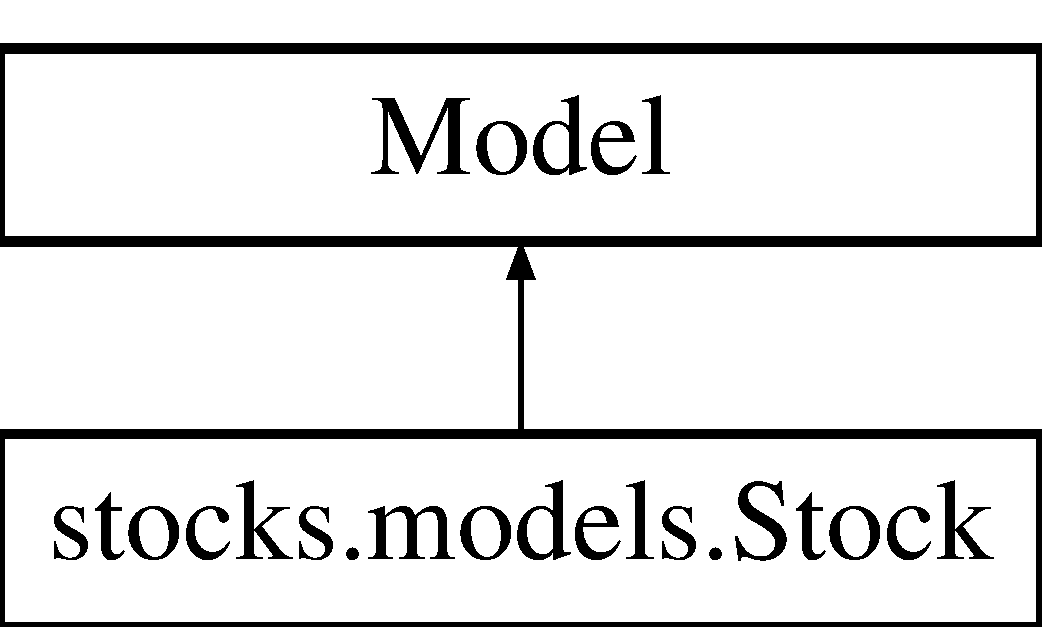
\includegraphics[height=2.000000cm]{classstocks_1_1models_1_1_stock}
\end{center}
\end{figure}
\subsection*{Static Public Attributes}
\begin{DoxyCompactItemize}
\item 
\mbox{\Hypertarget{classstocks_1_1models_1_1_stock_ad5b5e27b467a6d2ea2665ae7a1de579f}\label{classstocks_1_1models_1_1_stock_ad5b5e27b467a6d2ea2665ae7a1de579f}} 
{\bfseries ticker} = models.\+Char\+Field(max\+\_\+length=50)
\item 
\mbox{\Hypertarget{classstocks_1_1models_1_1_stock_afdadd827c199a742894ff1d25f4d238c}\label{classstocks_1_1models_1_1_stock_afdadd827c199a742894ff1d25f4d238c}} 
{\bfseries high} = models.\+Float\+Field(blank=True, default=0)
\item 
\mbox{\Hypertarget{classstocks_1_1models_1_1_stock_a9a64db423ee7f46e30860665d5b9a1d8}\label{classstocks_1_1models_1_1_stock_a9a64db423ee7f46e30860665d5b9a1d8}} 
{\bfseries low} = models.\+Float\+Field(blank=True, default=0)
\item 
\mbox{\Hypertarget{classstocks_1_1models_1_1_stock_a75d1102df2e6a2f79ee8ebff75500037}\label{classstocks_1_1models_1_1_stock_a75d1102df2e6a2f79ee8ebff75500037}} 
{\bfseries opening} = models.\+Float\+Field(blank=True, default=0)
\item 
\mbox{\Hypertarget{classstocks_1_1models_1_1_stock_a6d906d6ae8aa32a7009474f9a9a78bf4}\label{classstocks_1_1models_1_1_stock_a6d906d6ae8aa32a7009474f9a9a78bf4}} 
{\bfseries closing} = models.\+Float\+Field(blank=True, default=0)
\item 
\mbox{\Hypertarget{classstocks_1_1models_1_1_stock_a1c43b12207da4c6b6d06a9acf4e1fe20}\label{classstocks_1_1models_1_1_stock_a1c43b12207da4c6b6d06a9acf4e1fe20}} 
{\bfseries volume} = models.\+Integer\+Field(blank=True, default=0)
\item 
\mbox{\Hypertarget{classstocks_1_1models_1_1_stock_a4d79a50425afd2fe02c6e03a32161be9}\label{classstocks_1_1models_1_1_stock_a4d79a50425afd2fe02c6e03a32161be9}} 
{\bfseries date} = models.\+Date\+Field(blank=True, null=True)
\end{DoxyCompactItemize}


The documentation for this class was generated from the following file\+:\begin{DoxyCompactItemize}
\item 
backend/stocks/models.\+py\end{DoxyCompactItemize}

\hypertarget{classstocks_1_1views_1_1_stock_detail}{}\section{stocks.\+views.\+Stock\+Detail Class Reference}
\label{classstocks_1_1views_1_1_stock_detail}\index{stocks.\+views.\+Stock\+Detail@{stocks.\+views.\+Stock\+Detail}}
Inheritance diagram for stocks.\+views.\+Stock\+Detail\+:\begin{figure}[H]
\begin{center}
\leavevmode
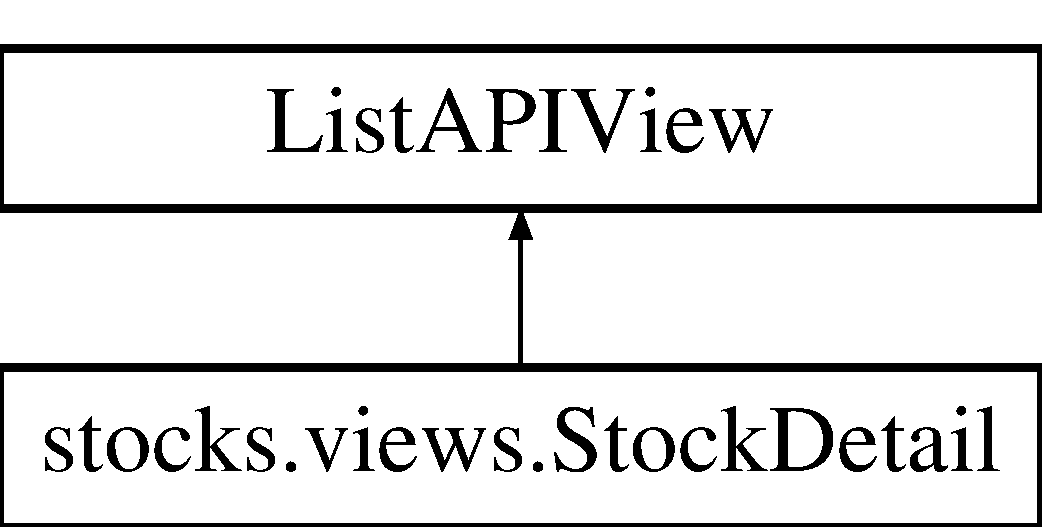
\includegraphics[height=2.000000cm]{classstocks_1_1views_1_1_stock_detail}
\end{center}
\end{figure}
\subsection*{Public Member Functions}
\begin{DoxyCompactItemize}
\item 
def \mbox{\hyperlink{classstocks_1_1views_1_1_stock_detail_a0fbaf7ab1f9964d060dce21b915c9aab}{get\+\_\+queryset}} (self)
\end{DoxyCompactItemize}
\subsection*{Static Public Attributes}
\begin{DoxyCompactItemize}
\item 
\mbox{\Hypertarget{classstocks_1_1views_1_1_stock_detail_aa723c51e7c9dfcca080fc9614637bec2}\label{classstocks_1_1views_1_1_stock_detail_aa723c51e7c9dfcca080fc9614637bec2}} 
{\bfseries serializer\+\_\+class} = \mbox{\hyperlink{classstocks_1_1serializers_1_1_stock_serializer}{Stock\+Serializer}}
\item 
\mbox{\Hypertarget{classstocks_1_1views_1_1_stock_detail_a6f1c51a040f506a50051d156afe457df}\label{classstocks_1_1views_1_1_stock_detail_a6f1c51a040f506a50051d156afe457df}} 
tuple {\bfseries filter\+\_\+backends} = (Ordering\+Filter,)
\item 
\mbox{\Hypertarget{classstocks_1_1views_1_1_stock_detail_a425b2803ff8e77804ae2e0b9b2e964f7}\label{classstocks_1_1views_1_1_stock_detail_a425b2803ff8e77804ae2e0b9b2e964f7}} 
tuple {\bfseries ordering\+\_\+fields} = (\textquotesingle{}date\textquotesingle{},)
\end{DoxyCompactItemize}


\subsection{Detailed Description}
\begin{DoxyVerb}This class creates view of one company's stock data, ordered by date.
\end{DoxyVerb}
 

\subsection{Member Function Documentation}
\mbox{\Hypertarget{classstocks_1_1views_1_1_stock_detail_a0fbaf7ab1f9964d060dce21b915c9aab}\label{classstocks_1_1views_1_1_stock_detail_a0fbaf7ab1f9964d060dce21b915c9aab}} 
\index{stocks\+::views\+::\+Stock\+Detail@{stocks\+::views\+::\+Stock\+Detail}!get\+\_\+queryset@{get\+\_\+queryset}}
\index{get\+\_\+queryset@{get\+\_\+queryset}!stocks\+::views\+::\+Stock\+Detail@{stocks\+::views\+::\+Stock\+Detail}}
\subsubsection{\texorpdfstring{get\+\_\+queryset()}{get\_queryset()}}
{\footnotesize\ttfamily def stocks.\+views.\+Stock\+Detail.\+get\+\_\+queryset (\begin{DoxyParamCaption}\item[{}]{self }\end{DoxyParamCaption})}

\begin{DoxyVerb}Override to check api key before getting queryset. Raises exception
if api key is not found in url parameters.
:return: AuthenticationFailed if no api key is provided,
 Http404 if company is invalid,
 otherwise queryset of data of one company.
\end{DoxyVerb}
 

The documentation for this class was generated from the following file\+:\begin{DoxyCompactItemize}
\item 
backend/stocks/views.\+py\end{DoxyCompactItemize}

\hypertarget{classstocks_1_1utilities_1_1_stock_history_updater}{}\section{stocks.\+utilities.\+Stock\+History\+Updater Class Reference}
\label{classstocks_1_1utilities_1_1_stock_history_updater}\index{stocks.\+utilities.\+Stock\+History\+Updater@{stocks.\+utilities.\+Stock\+History\+Updater}}
\subsection*{Static Public Member Functions}
\begin{DoxyCompactItemize}
\item 
def \mbox{\hyperlink{classstocks_1_1utilities_1_1_stock_history_updater_aa943ba0956fc5af74f69a32416d4246f}{update\+\_\+by\+\_\+ticker}} (ticker)
\item 
def \mbox{\hyperlink{classstocks_1_1utilities_1_1_stock_history_updater_ac26ce6122903a501fbc6144fe9808fed}{update\+\_\+all}} ()
\end{DoxyCompactItemize}


\subsection{Detailed Description}
\begin{DoxyVerb}Utility class to manage updates of history data on database.
Update on stock history should occur daily,
ideally after market closes.
\end{DoxyVerb}
 

\subsection{Member Function Documentation}
\mbox{\Hypertarget{classstocks_1_1utilities_1_1_stock_history_updater_ac26ce6122903a501fbc6144fe9808fed}\label{classstocks_1_1utilities_1_1_stock_history_updater_ac26ce6122903a501fbc6144fe9808fed}} 
\index{stocks\+::utilities\+::\+Stock\+History\+Updater@{stocks\+::utilities\+::\+Stock\+History\+Updater}!update\+\_\+all@{update\+\_\+all}}
\index{update\+\_\+all@{update\+\_\+all}!stocks\+::utilities\+::\+Stock\+History\+Updater@{stocks\+::utilities\+::\+Stock\+History\+Updater}}
\subsubsection{\texorpdfstring{update\+\_\+all()}{update\_all()}}
{\footnotesize\ttfamily def stocks.\+utilities.\+Stock\+History\+Updater.\+update\+\_\+all (\begin{DoxyParamCaption}{ }\end{DoxyParamCaption})\hspace{0.3cm}{\ttfamily [static]}}

\begin{DoxyVerb}Updates stock data for all companies in database using
Stock.update_by_ticker function.
:return: Operation result of update on each ticker
\end{DoxyVerb}
 \mbox{\Hypertarget{classstocks_1_1utilities_1_1_stock_history_updater_aa943ba0956fc5af74f69a32416d4246f}\label{classstocks_1_1utilities_1_1_stock_history_updater_aa943ba0956fc5af74f69a32416d4246f}} 
\index{stocks\+::utilities\+::\+Stock\+History\+Updater@{stocks\+::utilities\+::\+Stock\+History\+Updater}!update\+\_\+by\+\_\+ticker@{update\+\_\+by\+\_\+ticker}}
\index{update\+\_\+by\+\_\+ticker@{update\+\_\+by\+\_\+ticker}!stocks\+::utilities\+::\+Stock\+History\+Updater@{stocks\+::utilities\+::\+Stock\+History\+Updater}}
\subsubsection{\texorpdfstring{update\+\_\+by\+\_\+ticker()}{update\_by\_ticker()}}
{\footnotesize\ttfamily def stocks.\+utilities.\+Stock\+History\+Updater.\+update\+\_\+by\+\_\+ticker (\begin{DoxyParamCaption}\item[{}]{ticker }\end{DoxyParamCaption})\hspace{0.3cm}{\ttfamily [static]}}

\begin{DoxyVerb}Get recent stock data of given ticker from AlphaVantage API and POSTs
latest data to database, then DELETEs oldest data from database.
Fails if company doesn't exist in database or record for current
date exists.
:param ticker: Ticker symbol to update data
:return: 0: success
 1: record already exists
 2: company not found in database
 -1: undefined error
\end{DoxyVerb}
 

The documentation for this class was generated from the following file\+:\begin{DoxyCompactItemize}
\item 
backend/stocks/utilities.\+py\end{DoxyCompactItemize}

\hypertarget{classstocks_1_1views_1_1_stock_list}{}\section{stocks.\+views.\+Stock\+List Class Reference}
\label{classstocks_1_1views_1_1_stock_list}\index{stocks.\+views.\+Stock\+List@{stocks.\+views.\+Stock\+List}}
Inheritance diagram for stocks.\+views.\+Stock\+List\+:\begin{figure}[H]
\begin{center}
\leavevmode
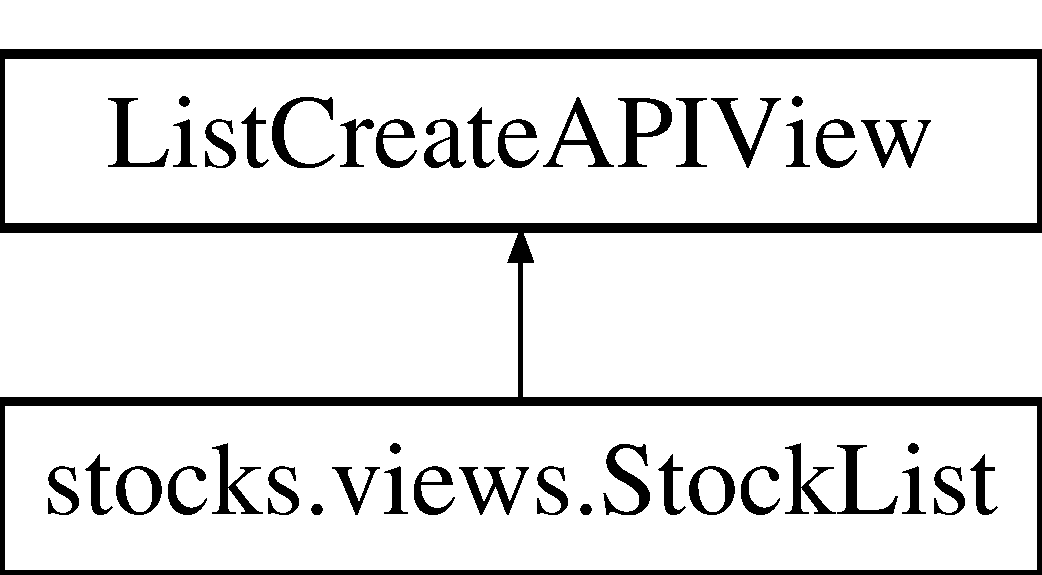
\includegraphics[height=2.000000cm]{classstocks_1_1views_1_1_stock_list}
\end{center}
\end{figure}
\subsection*{Public Member Functions}
\begin{DoxyCompactItemize}
\item 
def \mbox{\hyperlink{classstocks_1_1views_1_1_stock_list_a59e9ccb2be0430bbeef05167009e40c3}{get\+\_\+queryset}} (self)
\end{DoxyCompactItemize}
\subsection*{Static Public Attributes}
\begin{DoxyCompactItemize}
\item 
\mbox{\Hypertarget{classstocks_1_1views_1_1_stock_list_ab607663b56d4ef0e78f97b695b369726}\label{classstocks_1_1views_1_1_stock_list_ab607663b56d4ef0e78f97b695b369726}} 
{\bfseries serializer\+\_\+class} = \mbox{\hyperlink{classstocks_1_1serializers_1_1_stock_serializer}{Stock\+Serializer}}
\item 
\mbox{\Hypertarget{classstocks_1_1views_1_1_stock_list_a5760e75d23a65adac016fa30b93af9e4}\label{classstocks_1_1views_1_1_stock_list_a5760e75d23a65adac016fa30b93af9e4}} 
tuple {\bfseries filter\+\_\+backends} = (Ordering\+Filter,)
\item 
\mbox{\Hypertarget{classstocks_1_1views_1_1_stock_list_a89797d122ada805421dcf12b2b4b680f}\label{classstocks_1_1views_1_1_stock_list_a89797d122ada805421dcf12b2b4b680f}} 
tuple {\bfseries ordering\+\_\+fields} = (\textquotesingle{}date\textquotesingle{},)
\end{DoxyCompactItemize}


\subsection{Detailed Description}
\begin{DoxyVerb}This class create view of all stock data in database, ordered by date.
\end{DoxyVerb}
 

\subsection{Member Function Documentation}
\mbox{\Hypertarget{classstocks_1_1views_1_1_stock_list_a59e9ccb2be0430bbeef05167009e40c3}\label{classstocks_1_1views_1_1_stock_list_a59e9ccb2be0430bbeef05167009e40c3}} 
\index{stocks\+::views\+::\+Stock\+List@{stocks\+::views\+::\+Stock\+List}!get\+\_\+queryset@{get\+\_\+queryset}}
\index{get\+\_\+queryset@{get\+\_\+queryset}!stocks\+::views\+::\+Stock\+List@{stocks\+::views\+::\+Stock\+List}}
\subsubsection{\texorpdfstring{get\+\_\+queryset()}{get\_queryset()}}
{\footnotesize\ttfamily def stocks.\+views.\+Stock\+List.\+get\+\_\+queryset (\begin{DoxyParamCaption}\item[{}]{self }\end{DoxyParamCaption})}

\begin{DoxyVerb}Override to check api key before getting queryset. Raises exception
if api key is not found in url parameters.
:return: AuthenticationFailed if no api key is provided,
 otherwise queryset of all stock data in database
\end{DoxyVerb}
 

The documentation for this class was generated from the following file\+:\begin{DoxyCompactItemize}
\item 
backend/stocks/views.\+py\end{DoxyCompactItemize}

\hypertarget{classstocks_1_1apps_1_1_stocks_config}{}\section{stocks.\+apps.\+Stocks\+Config Class Reference}
\label{classstocks_1_1apps_1_1_stocks_config}\index{stocks.\+apps.\+Stocks\+Config@{stocks.\+apps.\+Stocks\+Config}}
Inheritance diagram for stocks.\+apps.\+Stocks\+Config\+:\begin{figure}[H]
\begin{center}
\leavevmode
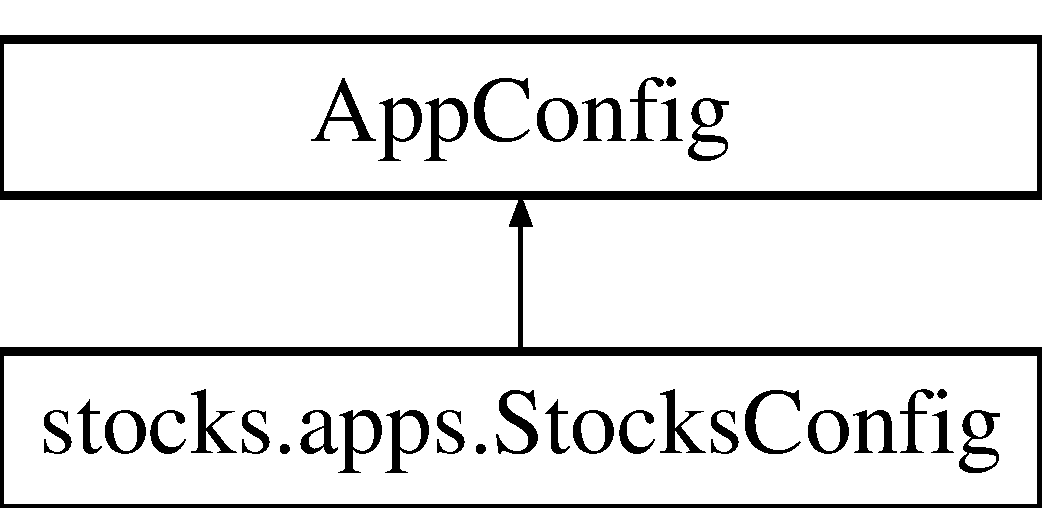
\includegraphics[height=2.000000cm]{classstocks_1_1apps_1_1_stocks_config}
\end{center}
\end{figure}
\subsection*{Static Public Attributes}
\begin{DoxyCompactItemize}
\item 
\mbox{\Hypertarget{classstocks_1_1apps_1_1_stocks_config_a03c22491b56cbcf361424667992e02cb}\label{classstocks_1_1apps_1_1_stocks_config_a03c22491b56cbcf361424667992e02cb}} 
string {\bfseries name} = \textquotesingle{}stocks\textquotesingle{}
\end{DoxyCompactItemize}


The documentation for this class was generated from the following file\+:\begin{DoxyCompactItemize}
\item 
backend/stocks/apps.\+py\end{DoxyCompactItemize}

\hypertarget{classstocks_1_1serializers_1_1_stock_serializer}{}\section{stocks.\+serializers.\+Stock\+Serializer Class Reference}
\label{classstocks_1_1serializers_1_1_stock_serializer}\index{stocks.\+serializers.\+Stock\+Serializer@{stocks.\+serializers.\+Stock\+Serializer}}
Inheritance diagram for stocks.\+serializers.\+Stock\+Serializer\+:\begin{figure}[H]
\begin{center}
\leavevmode
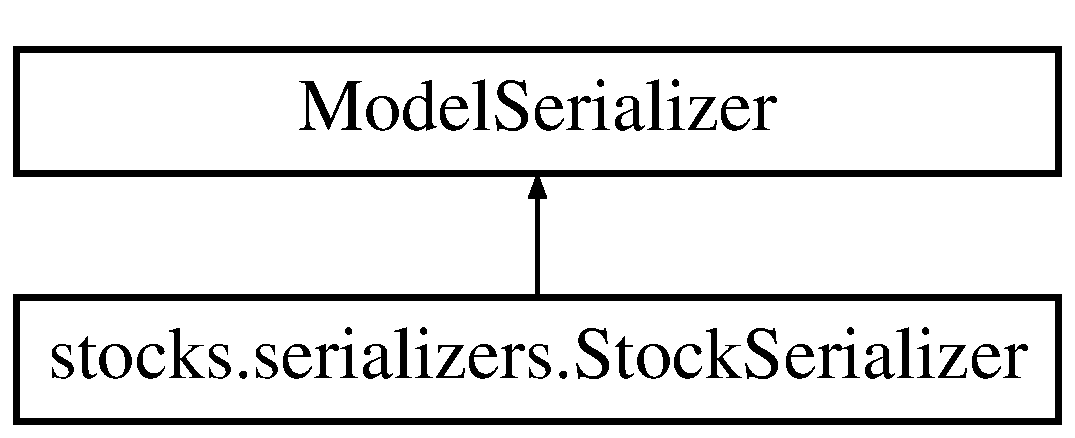
\includegraphics[height=2.000000cm]{classstocks_1_1serializers_1_1_stock_serializer}
\end{center}
\end{figure}
\subsection*{Classes}
\begin{DoxyCompactItemize}
\item 
class \mbox{\hyperlink{classstocks_1_1serializers_1_1_stock_serializer_1_1_meta}{Meta}}
\end{DoxyCompactItemize}


The documentation for this class was generated from the following file\+:\begin{DoxyCompactItemize}
\item 
backend/stocks/serializers.\+py\end{DoxyCompactItemize}

\hypertarget{classdata__mine_1_1tests_1_1test__stock_1_1_stock_test_case}{}\section{data\+\_\+mine.\+tests.\+test\+\_\+stock.\+Stock\+Test\+Case Class Reference}
\label{classdata__mine_1_1tests_1_1test__stock_1_1_stock_test_case}\index{data\+\_\+mine.\+tests.\+test\+\_\+stock.\+Stock\+Test\+Case@{data\+\_\+mine.\+tests.\+test\+\_\+stock.\+Stock\+Test\+Case}}
Inheritance diagram for data\+\_\+mine.\+tests.\+test\+\_\+stock.\+Stock\+Test\+Case\+:\begin{figure}[H]
\begin{center}
\leavevmode
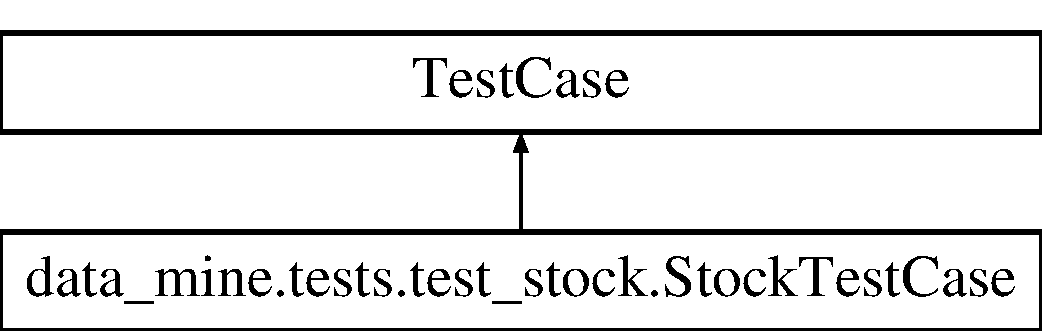
\includegraphics[height=2.000000cm]{classdata__mine_1_1tests_1_1test__stock_1_1_stock_test_case}
\end{center}
\end{figure}
\subsection*{Public Member Functions}
\begin{DoxyCompactItemize}
\item 
\mbox{\Hypertarget{classdata__mine_1_1tests_1_1test__stock_1_1_stock_test_case_abaeea6624818de33babf97a7f998ac17}\label{classdata__mine_1_1tests_1_1test__stock_1_1_stock_test_case_abaeea6624818de33babf97a7f998ac17}} 
def {\bfseries set\+Up\+Test\+Data} (self)
\item 
\mbox{\Hypertarget{classdata__mine_1_1tests_1_1test__stock_1_1_stock_test_case_abde0115a4959c0a54133efdab742993c}\label{classdata__mine_1_1tests_1_1test__stock_1_1_stock_test_case_abde0115a4959c0a54133efdab742993c}} 
def {\bfseries test\+\_\+stock\+\_\+create} (self)
\end{DoxyCompactItemize}


The documentation for this class was generated from the following file\+:\begin{DoxyCompactItemize}
\item 
backend/data\+\_\+mine/tests/test\+\_\+stock.\+py\end{DoxyCompactItemize}

\hypertarget{classstocks_1_1tests_1_1_view_test_case}{}\section{stocks.\+tests.\+View\+Test\+Case Class Reference}
\label{classstocks_1_1tests_1_1_view_test_case}\index{stocks.\+tests.\+View\+Test\+Case@{stocks.\+tests.\+View\+Test\+Case}}
Inheritance diagram for stocks.\+tests.\+View\+Test\+Case\+:\begin{figure}[H]
\begin{center}
\leavevmode
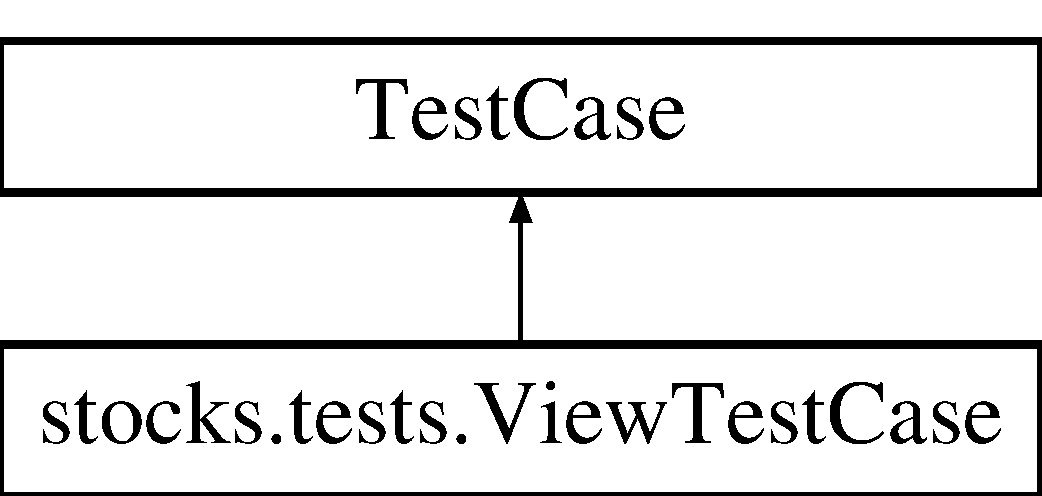
\includegraphics[height=2.000000cm]{classstocks_1_1tests_1_1_view_test_case}
\end{center}
\end{figure}
\subsection*{Public Member Functions}
\begin{DoxyCompactItemize}
\item 
def \mbox{\hyperlink{classstocks_1_1tests_1_1_view_test_case_aeeb77affba267291807c3166878695b0}{test\+\_\+get\+\_\+stock\+\_\+history}} (self)
\item 
def \mbox{\hyperlink{classstocks_1_1tests_1_1_view_test_case_a5c517912eeb301485cf9348c1a15c337}{test\+\_\+get\+\_\+invalid\+\_\+stock\+\_\+history}} (self)
\item 
def \mbox{\hyperlink{classstocks_1_1tests_1_1_view_test_case_a9c483c27402609a2dee5464659d8fc0f}{test\+\_\+get\+\_\+stock\+\_\+history\+\_\+api\+\_\+key\+\_\+check}} (self)
\item 
def \mbox{\hyperlink{classstocks_1_1tests_1_1_view_test_case_ac2f58bc80e6aa03c3998c2bc6f55f339}{test\+\_\+get\+\_\+stock\+\_\+history\+\_\+invalid\+\_\+api\+\_\+key}} (self)
\item 
def \mbox{\hyperlink{classstocks_1_1tests_1_1_view_test_case_a86133da39156dbaa0091060ede0481aa}{test\+\_\+get\+\_\+all\+\_\+stock\+\_\+history}} (self)
\item 
def \mbox{\hyperlink{classstocks_1_1tests_1_1_view_test_case_a39ae95c8302a02d768ab763ea5ec7516}{test\+\_\+get\+\_\+all\+\_\+stock\+\_\+history\+\_\+api\+\_\+key\+\_\+check}} (self)
\item 
def \mbox{\hyperlink{classstocks_1_1tests_1_1_view_test_case_ae5a47bd1dada19b0c52707a79b46d71f}{test\+\_\+get\+\_\+all\+\_\+stock\+\_\+history\+\_\+invalid\+\_\+api\+\_\+key}} (self)
\item 
def \mbox{\hyperlink{classstocks_1_1tests_1_1_view_test_case_a55bfe0efa26d9744e8deff494b3efa44}{test\+\_\+run\+\_\+experiment}} (self)
\item 
def \mbox{\hyperlink{classstocks_1_1tests_1_1_view_test_case_aff28edc2c2f360e277d6df4aa76bb360}{test\+\_\+run\+\_\+invalid\+\_\+experiment}} (self)
\item 
def \mbox{\hyperlink{classstocks_1_1tests_1_1_view_test_case_aa70044a70ede048d43709cf890cc3587}{test\+\_\+run\+\_\+experiment\+\_\+api\+\_\+key\+\_\+check}} (self)
\item 
def \mbox{\hyperlink{classstocks_1_1tests_1_1_view_test_case_ab44cd3675788ad59ea5fd4d6e37903f2}{test\+\_\+run\+\_\+experiment\+\_\+invalid\+\_\+api\+\_\+key}} (self)
\item 
def \mbox{\hyperlink{classstocks_1_1tests_1_1_view_test_case_a0583f6d1895e7a98e9156fb01ca785a2}{test\+\_\+update\+\_\+ticker}} (self)
\item 
def \mbox{\hyperlink{classstocks_1_1tests_1_1_view_test_case_a0794c69e03de1cf85ee490f0bf6be5e2}{test\+\_\+update\+\_\+ticker\+\_\+already\+\_\+latest}} (self)
\item 
def \mbox{\hyperlink{classstocks_1_1tests_1_1_view_test_case_a122a576c4be868f941a7d1fca2c5c188}{test\+\_\+update\+\_\+invalid\+\_\+ticker}} (self)
\item 
def \mbox{\hyperlink{classstocks_1_1tests_1_1_view_test_case_a61c3bdc301ef40c84704d8b2630d62bb}{test\+\_\+update\+\_\+ticker\+\_\+api\+\_\+key\+\_\+check}} (self)
\item 
def \mbox{\hyperlink{classstocks_1_1tests_1_1_view_test_case_ad0f6d1743dfa3ee2e681000b9246b892}{test\+\_\+update\+\_\+ticker\+\_\+invalid\+\_\+api\+\_\+key}} (self)
\item 
def \mbox{\hyperlink{classstocks_1_1tests_1_1_view_test_case_ab802f27159bdbc80348a17d2370e0f8a}{test\+\_\+update\+\_\+all}} (self)
\item 
def \mbox{\hyperlink{classstocks_1_1tests_1_1_view_test_case_adaa6a206656cb4a9c05f7376f6b15461}{test\+\_\+update\+\_\+all\+\_\+existing}} (self)
\item 
def \mbox{\hyperlink{classstocks_1_1tests_1_1_view_test_case_a3d75983e03c72099b81b70c4918998ab}{test\+\_\+update\+\_\+all\+\_\+api\+\_\+key\+\_\+check}} (self)
\item 
def \mbox{\hyperlink{classstocks_1_1tests_1_1_view_test_case_adc732cc51d49e4ab5503098f996ff78b}{test\+\_\+update\+\_\+all\+\_\+invalid\+\_\+api\+\_\+key}} (self)
\end{DoxyCompactItemize}


\subsection{Member Function Documentation}
\mbox{\Hypertarget{classstocks_1_1tests_1_1_view_test_case_a86133da39156dbaa0091060ede0481aa}\label{classstocks_1_1tests_1_1_view_test_case_a86133da39156dbaa0091060ede0481aa}} 
\index{stocks\+::tests\+::\+View\+Test\+Case@{stocks\+::tests\+::\+View\+Test\+Case}!test\+\_\+get\+\_\+all\+\_\+stock\+\_\+history@{test\+\_\+get\+\_\+all\+\_\+stock\+\_\+history}}
\index{test\+\_\+get\+\_\+all\+\_\+stock\+\_\+history@{test\+\_\+get\+\_\+all\+\_\+stock\+\_\+history}!stocks\+::tests\+::\+View\+Test\+Case@{stocks\+::tests\+::\+View\+Test\+Case}}
\subsubsection{\texorpdfstring{test\+\_\+get\+\_\+all\+\_\+stock\+\_\+history()}{test\_get\_all\_stock\_history()}}
{\footnotesize\ttfamily def stocks.\+tests.\+View\+Test\+Case.\+test\+\_\+get\+\_\+all\+\_\+stock\+\_\+history (\begin{DoxyParamCaption}\item[{}]{self }\end{DoxyParamCaption})}

\begin{DoxyVerb}Tests valid /stocks endpoint call.
\end{DoxyVerb}
 \mbox{\Hypertarget{classstocks_1_1tests_1_1_view_test_case_a39ae95c8302a02d768ab763ea5ec7516}\label{classstocks_1_1tests_1_1_view_test_case_a39ae95c8302a02d768ab763ea5ec7516}} 
\index{stocks\+::tests\+::\+View\+Test\+Case@{stocks\+::tests\+::\+View\+Test\+Case}!test\+\_\+get\+\_\+all\+\_\+stock\+\_\+history\+\_\+api\+\_\+key\+\_\+check@{test\+\_\+get\+\_\+all\+\_\+stock\+\_\+history\+\_\+api\+\_\+key\+\_\+check}}
\index{test\+\_\+get\+\_\+all\+\_\+stock\+\_\+history\+\_\+api\+\_\+key\+\_\+check@{test\+\_\+get\+\_\+all\+\_\+stock\+\_\+history\+\_\+api\+\_\+key\+\_\+check}!stocks\+::tests\+::\+View\+Test\+Case@{stocks\+::tests\+::\+View\+Test\+Case}}
\subsubsection{\texorpdfstring{test\+\_\+get\+\_\+all\+\_\+stock\+\_\+history\+\_\+api\+\_\+key\+\_\+check()}{test\_get\_all\_stock\_history\_api\_key\_check()}}
{\footnotesize\ttfamily def stocks.\+tests.\+View\+Test\+Case.\+test\+\_\+get\+\_\+all\+\_\+stock\+\_\+history\+\_\+api\+\_\+key\+\_\+check (\begin{DoxyParamCaption}\item[{}]{self }\end{DoxyParamCaption})}

\begin{DoxyVerb}Tests /stocks endpoint call without api key.
\end{DoxyVerb}
 \mbox{\Hypertarget{classstocks_1_1tests_1_1_view_test_case_ae5a47bd1dada19b0c52707a79b46d71f}\label{classstocks_1_1tests_1_1_view_test_case_ae5a47bd1dada19b0c52707a79b46d71f}} 
\index{stocks\+::tests\+::\+View\+Test\+Case@{stocks\+::tests\+::\+View\+Test\+Case}!test\+\_\+get\+\_\+all\+\_\+stock\+\_\+history\+\_\+invalid\+\_\+api\+\_\+key@{test\+\_\+get\+\_\+all\+\_\+stock\+\_\+history\+\_\+invalid\+\_\+api\+\_\+key}}
\index{test\+\_\+get\+\_\+all\+\_\+stock\+\_\+history\+\_\+invalid\+\_\+api\+\_\+key@{test\+\_\+get\+\_\+all\+\_\+stock\+\_\+history\+\_\+invalid\+\_\+api\+\_\+key}!stocks\+::tests\+::\+View\+Test\+Case@{stocks\+::tests\+::\+View\+Test\+Case}}
\subsubsection{\texorpdfstring{test\+\_\+get\+\_\+all\+\_\+stock\+\_\+history\+\_\+invalid\+\_\+api\+\_\+key()}{test\_get\_all\_stock\_history\_invalid\_api\_key()}}
{\footnotesize\ttfamily def stocks.\+tests.\+View\+Test\+Case.\+test\+\_\+get\+\_\+all\+\_\+stock\+\_\+history\+\_\+invalid\+\_\+api\+\_\+key (\begin{DoxyParamCaption}\item[{}]{self }\end{DoxyParamCaption})}

\begin{DoxyVerb}Tests /stocks endpoint call with wrong api key.
\end{DoxyVerb}
 \mbox{\Hypertarget{classstocks_1_1tests_1_1_view_test_case_a5c517912eeb301485cf9348c1a15c337}\label{classstocks_1_1tests_1_1_view_test_case_a5c517912eeb301485cf9348c1a15c337}} 
\index{stocks\+::tests\+::\+View\+Test\+Case@{stocks\+::tests\+::\+View\+Test\+Case}!test\+\_\+get\+\_\+invalid\+\_\+stock\+\_\+history@{test\+\_\+get\+\_\+invalid\+\_\+stock\+\_\+history}}
\index{test\+\_\+get\+\_\+invalid\+\_\+stock\+\_\+history@{test\+\_\+get\+\_\+invalid\+\_\+stock\+\_\+history}!stocks\+::tests\+::\+View\+Test\+Case@{stocks\+::tests\+::\+View\+Test\+Case}}
\subsubsection{\texorpdfstring{test\+\_\+get\+\_\+invalid\+\_\+stock\+\_\+history()}{test\_get\_invalid\_stock\_history()}}
{\footnotesize\ttfamily def stocks.\+tests.\+View\+Test\+Case.\+test\+\_\+get\+\_\+invalid\+\_\+stock\+\_\+history (\begin{DoxyParamCaption}\item[{}]{self }\end{DoxyParamCaption})}

\begin{DoxyVerb}Tests /stocks/<ticker> endpoint call on non-existing company.
\end{DoxyVerb}
 \mbox{\Hypertarget{classstocks_1_1tests_1_1_view_test_case_aeeb77affba267291807c3166878695b0}\label{classstocks_1_1tests_1_1_view_test_case_aeeb77affba267291807c3166878695b0}} 
\index{stocks\+::tests\+::\+View\+Test\+Case@{stocks\+::tests\+::\+View\+Test\+Case}!test\+\_\+get\+\_\+stock\+\_\+history@{test\+\_\+get\+\_\+stock\+\_\+history}}
\index{test\+\_\+get\+\_\+stock\+\_\+history@{test\+\_\+get\+\_\+stock\+\_\+history}!stocks\+::tests\+::\+View\+Test\+Case@{stocks\+::tests\+::\+View\+Test\+Case}}
\subsubsection{\texorpdfstring{test\+\_\+get\+\_\+stock\+\_\+history()}{test\_get\_stock\_history()}}
{\footnotesize\ttfamily def stocks.\+tests.\+View\+Test\+Case.\+test\+\_\+get\+\_\+stock\+\_\+history (\begin{DoxyParamCaption}\item[{}]{self }\end{DoxyParamCaption})}

\begin{DoxyVerb}Tests valid /stocks/<ticker> endpoint call.
\end{DoxyVerb}
 \mbox{\Hypertarget{classstocks_1_1tests_1_1_view_test_case_a9c483c27402609a2dee5464659d8fc0f}\label{classstocks_1_1tests_1_1_view_test_case_a9c483c27402609a2dee5464659d8fc0f}} 
\index{stocks\+::tests\+::\+View\+Test\+Case@{stocks\+::tests\+::\+View\+Test\+Case}!test\+\_\+get\+\_\+stock\+\_\+history\+\_\+api\+\_\+key\+\_\+check@{test\+\_\+get\+\_\+stock\+\_\+history\+\_\+api\+\_\+key\+\_\+check}}
\index{test\+\_\+get\+\_\+stock\+\_\+history\+\_\+api\+\_\+key\+\_\+check@{test\+\_\+get\+\_\+stock\+\_\+history\+\_\+api\+\_\+key\+\_\+check}!stocks\+::tests\+::\+View\+Test\+Case@{stocks\+::tests\+::\+View\+Test\+Case}}
\subsubsection{\texorpdfstring{test\+\_\+get\+\_\+stock\+\_\+history\+\_\+api\+\_\+key\+\_\+check()}{test\_get\_stock\_history\_api\_key\_check()}}
{\footnotesize\ttfamily def stocks.\+tests.\+View\+Test\+Case.\+test\+\_\+get\+\_\+stock\+\_\+history\+\_\+api\+\_\+key\+\_\+check (\begin{DoxyParamCaption}\item[{}]{self }\end{DoxyParamCaption})}

\begin{DoxyVerb}Tests /stocks/<ticker> endpoint call without api key.
\end{DoxyVerb}
 \mbox{\Hypertarget{classstocks_1_1tests_1_1_view_test_case_ac2f58bc80e6aa03c3998c2bc6f55f339}\label{classstocks_1_1tests_1_1_view_test_case_ac2f58bc80e6aa03c3998c2bc6f55f339}} 
\index{stocks\+::tests\+::\+View\+Test\+Case@{stocks\+::tests\+::\+View\+Test\+Case}!test\+\_\+get\+\_\+stock\+\_\+history\+\_\+invalid\+\_\+api\+\_\+key@{test\+\_\+get\+\_\+stock\+\_\+history\+\_\+invalid\+\_\+api\+\_\+key}}
\index{test\+\_\+get\+\_\+stock\+\_\+history\+\_\+invalid\+\_\+api\+\_\+key@{test\+\_\+get\+\_\+stock\+\_\+history\+\_\+invalid\+\_\+api\+\_\+key}!stocks\+::tests\+::\+View\+Test\+Case@{stocks\+::tests\+::\+View\+Test\+Case}}
\subsubsection{\texorpdfstring{test\+\_\+get\+\_\+stock\+\_\+history\+\_\+invalid\+\_\+api\+\_\+key()}{test\_get\_stock\_history\_invalid\_api\_key()}}
{\footnotesize\ttfamily def stocks.\+tests.\+View\+Test\+Case.\+test\+\_\+get\+\_\+stock\+\_\+history\+\_\+invalid\+\_\+api\+\_\+key (\begin{DoxyParamCaption}\item[{}]{self }\end{DoxyParamCaption})}

\begin{DoxyVerb}Tests /stocks/<ticker> endpoint call with wrong api key.
\end{DoxyVerb}
 \mbox{\Hypertarget{classstocks_1_1tests_1_1_view_test_case_a55bfe0efa26d9744e8deff494b3efa44}\label{classstocks_1_1tests_1_1_view_test_case_a55bfe0efa26d9744e8deff494b3efa44}} 
\index{stocks\+::tests\+::\+View\+Test\+Case@{stocks\+::tests\+::\+View\+Test\+Case}!test\+\_\+run\+\_\+experiment@{test\+\_\+run\+\_\+experiment}}
\index{test\+\_\+run\+\_\+experiment@{test\+\_\+run\+\_\+experiment}!stocks\+::tests\+::\+View\+Test\+Case@{stocks\+::tests\+::\+View\+Test\+Case}}
\subsubsection{\texorpdfstring{test\+\_\+run\+\_\+experiment()}{test\_run\_experiment()}}
{\footnotesize\ttfamily def stocks.\+tests.\+View\+Test\+Case.\+test\+\_\+run\+\_\+experiment (\begin{DoxyParamCaption}\item[{}]{self }\end{DoxyParamCaption})}

\begin{DoxyVerb}Tests valid /stocks/<ticker>/runexpr endpoint call.
\end{DoxyVerb}
 \mbox{\Hypertarget{classstocks_1_1tests_1_1_view_test_case_aa70044a70ede048d43709cf890cc3587}\label{classstocks_1_1tests_1_1_view_test_case_aa70044a70ede048d43709cf890cc3587}} 
\index{stocks\+::tests\+::\+View\+Test\+Case@{stocks\+::tests\+::\+View\+Test\+Case}!test\+\_\+run\+\_\+experiment\+\_\+api\+\_\+key\+\_\+check@{test\+\_\+run\+\_\+experiment\+\_\+api\+\_\+key\+\_\+check}}
\index{test\+\_\+run\+\_\+experiment\+\_\+api\+\_\+key\+\_\+check@{test\+\_\+run\+\_\+experiment\+\_\+api\+\_\+key\+\_\+check}!stocks\+::tests\+::\+View\+Test\+Case@{stocks\+::tests\+::\+View\+Test\+Case}}
\subsubsection{\texorpdfstring{test\+\_\+run\+\_\+experiment\+\_\+api\+\_\+key\+\_\+check()}{test\_run\_experiment\_api\_key\_check()}}
{\footnotesize\ttfamily def stocks.\+tests.\+View\+Test\+Case.\+test\+\_\+run\+\_\+experiment\+\_\+api\+\_\+key\+\_\+check (\begin{DoxyParamCaption}\item[{}]{self }\end{DoxyParamCaption})}

\begin{DoxyVerb}Tests /stocks/<ticker>/runexpr endpoint call without api key.
\end{DoxyVerb}
 \mbox{\Hypertarget{classstocks_1_1tests_1_1_view_test_case_ab44cd3675788ad59ea5fd4d6e37903f2}\label{classstocks_1_1tests_1_1_view_test_case_ab44cd3675788ad59ea5fd4d6e37903f2}} 
\index{stocks\+::tests\+::\+View\+Test\+Case@{stocks\+::tests\+::\+View\+Test\+Case}!test\+\_\+run\+\_\+experiment\+\_\+invalid\+\_\+api\+\_\+key@{test\+\_\+run\+\_\+experiment\+\_\+invalid\+\_\+api\+\_\+key}}
\index{test\+\_\+run\+\_\+experiment\+\_\+invalid\+\_\+api\+\_\+key@{test\+\_\+run\+\_\+experiment\+\_\+invalid\+\_\+api\+\_\+key}!stocks\+::tests\+::\+View\+Test\+Case@{stocks\+::tests\+::\+View\+Test\+Case}}
\subsubsection{\texorpdfstring{test\+\_\+run\+\_\+experiment\+\_\+invalid\+\_\+api\+\_\+key()}{test\_run\_experiment\_invalid\_api\_key()}}
{\footnotesize\ttfamily def stocks.\+tests.\+View\+Test\+Case.\+test\+\_\+run\+\_\+experiment\+\_\+invalid\+\_\+api\+\_\+key (\begin{DoxyParamCaption}\item[{}]{self }\end{DoxyParamCaption})}

\begin{DoxyVerb}Tests /stocks/<ticker>/runexpr endpoint call with wrong api key.
\end{DoxyVerb}
 \mbox{\Hypertarget{classstocks_1_1tests_1_1_view_test_case_aff28edc2c2f360e277d6df4aa76bb360}\label{classstocks_1_1tests_1_1_view_test_case_aff28edc2c2f360e277d6df4aa76bb360}} 
\index{stocks\+::tests\+::\+View\+Test\+Case@{stocks\+::tests\+::\+View\+Test\+Case}!test\+\_\+run\+\_\+invalid\+\_\+experiment@{test\+\_\+run\+\_\+invalid\+\_\+experiment}}
\index{test\+\_\+run\+\_\+invalid\+\_\+experiment@{test\+\_\+run\+\_\+invalid\+\_\+experiment}!stocks\+::tests\+::\+View\+Test\+Case@{stocks\+::tests\+::\+View\+Test\+Case}}
\subsubsection{\texorpdfstring{test\+\_\+run\+\_\+invalid\+\_\+experiment()}{test\_run\_invalid\_experiment()}}
{\footnotesize\ttfamily def stocks.\+tests.\+View\+Test\+Case.\+test\+\_\+run\+\_\+invalid\+\_\+experiment (\begin{DoxyParamCaption}\item[{}]{self }\end{DoxyParamCaption})}

\begin{DoxyVerb}Tests /stocks/<ticker>/runexpr endpoint call on non-existing company.
:return:
\end{DoxyVerb}
 \mbox{\Hypertarget{classstocks_1_1tests_1_1_view_test_case_ab802f27159bdbc80348a17d2370e0f8a}\label{classstocks_1_1tests_1_1_view_test_case_ab802f27159bdbc80348a17d2370e0f8a}} 
\index{stocks\+::tests\+::\+View\+Test\+Case@{stocks\+::tests\+::\+View\+Test\+Case}!test\+\_\+update\+\_\+all@{test\+\_\+update\+\_\+all}}
\index{test\+\_\+update\+\_\+all@{test\+\_\+update\+\_\+all}!stocks\+::tests\+::\+View\+Test\+Case@{stocks\+::tests\+::\+View\+Test\+Case}}
\subsubsection{\texorpdfstring{test\+\_\+update\+\_\+all()}{test\_update\_all()}}
{\footnotesize\ttfamily def stocks.\+tests.\+View\+Test\+Case.\+test\+\_\+update\+\_\+all (\begin{DoxyParamCaption}\item[{}]{self }\end{DoxyParamCaption})}

\begin{DoxyVerb}Tests valid /stocks/update endpoint call.
\end{DoxyVerb}
 \mbox{\Hypertarget{classstocks_1_1tests_1_1_view_test_case_a3d75983e03c72099b81b70c4918998ab}\label{classstocks_1_1tests_1_1_view_test_case_a3d75983e03c72099b81b70c4918998ab}} 
\index{stocks\+::tests\+::\+View\+Test\+Case@{stocks\+::tests\+::\+View\+Test\+Case}!test\+\_\+update\+\_\+all\+\_\+api\+\_\+key\+\_\+check@{test\+\_\+update\+\_\+all\+\_\+api\+\_\+key\+\_\+check}}
\index{test\+\_\+update\+\_\+all\+\_\+api\+\_\+key\+\_\+check@{test\+\_\+update\+\_\+all\+\_\+api\+\_\+key\+\_\+check}!stocks\+::tests\+::\+View\+Test\+Case@{stocks\+::tests\+::\+View\+Test\+Case}}
\subsubsection{\texorpdfstring{test\+\_\+update\+\_\+all\+\_\+api\+\_\+key\+\_\+check()}{test\_update\_all\_api\_key\_check()}}
{\footnotesize\ttfamily def stocks.\+tests.\+View\+Test\+Case.\+test\+\_\+update\+\_\+all\+\_\+api\+\_\+key\+\_\+check (\begin{DoxyParamCaption}\item[{}]{self }\end{DoxyParamCaption})}

\begin{DoxyVerb}Tests /stocks/update endpoint call without api key.
\end{DoxyVerb}
 \mbox{\Hypertarget{classstocks_1_1tests_1_1_view_test_case_adaa6a206656cb4a9c05f7376f6b15461}\label{classstocks_1_1tests_1_1_view_test_case_adaa6a206656cb4a9c05f7376f6b15461}} 
\index{stocks\+::tests\+::\+View\+Test\+Case@{stocks\+::tests\+::\+View\+Test\+Case}!test\+\_\+update\+\_\+all\+\_\+existing@{test\+\_\+update\+\_\+all\+\_\+existing}}
\index{test\+\_\+update\+\_\+all\+\_\+existing@{test\+\_\+update\+\_\+all\+\_\+existing}!stocks\+::tests\+::\+View\+Test\+Case@{stocks\+::tests\+::\+View\+Test\+Case}}
\subsubsection{\texorpdfstring{test\+\_\+update\+\_\+all\+\_\+existing()}{test\_update\_all\_existing()}}
{\footnotesize\ttfamily def stocks.\+tests.\+View\+Test\+Case.\+test\+\_\+update\+\_\+all\+\_\+existing (\begin{DoxyParamCaption}\item[{}]{self }\end{DoxyParamCaption})}

\begin{DoxyVerb}Tests /stocks/update endpoint call, with some data already
up to date in database.
\end{DoxyVerb}
 \mbox{\Hypertarget{classstocks_1_1tests_1_1_view_test_case_adc732cc51d49e4ab5503098f996ff78b}\label{classstocks_1_1tests_1_1_view_test_case_adc732cc51d49e4ab5503098f996ff78b}} 
\index{stocks\+::tests\+::\+View\+Test\+Case@{stocks\+::tests\+::\+View\+Test\+Case}!test\+\_\+update\+\_\+all\+\_\+invalid\+\_\+api\+\_\+key@{test\+\_\+update\+\_\+all\+\_\+invalid\+\_\+api\+\_\+key}}
\index{test\+\_\+update\+\_\+all\+\_\+invalid\+\_\+api\+\_\+key@{test\+\_\+update\+\_\+all\+\_\+invalid\+\_\+api\+\_\+key}!stocks\+::tests\+::\+View\+Test\+Case@{stocks\+::tests\+::\+View\+Test\+Case}}
\subsubsection{\texorpdfstring{test\+\_\+update\+\_\+all\+\_\+invalid\+\_\+api\+\_\+key()}{test\_update\_all\_invalid\_api\_key()}}
{\footnotesize\ttfamily def stocks.\+tests.\+View\+Test\+Case.\+test\+\_\+update\+\_\+all\+\_\+invalid\+\_\+api\+\_\+key (\begin{DoxyParamCaption}\item[{}]{self }\end{DoxyParamCaption})}

\begin{DoxyVerb}Tests /stocks/update endpoint call with wrong api key.
\end{DoxyVerb}
 \mbox{\Hypertarget{classstocks_1_1tests_1_1_view_test_case_a122a576c4be868f941a7d1fca2c5c188}\label{classstocks_1_1tests_1_1_view_test_case_a122a576c4be868f941a7d1fca2c5c188}} 
\index{stocks\+::tests\+::\+View\+Test\+Case@{stocks\+::tests\+::\+View\+Test\+Case}!test\+\_\+update\+\_\+invalid\+\_\+ticker@{test\+\_\+update\+\_\+invalid\+\_\+ticker}}
\index{test\+\_\+update\+\_\+invalid\+\_\+ticker@{test\+\_\+update\+\_\+invalid\+\_\+ticker}!stocks\+::tests\+::\+View\+Test\+Case@{stocks\+::tests\+::\+View\+Test\+Case}}
\subsubsection{\texorpdfstring{test\+\_\+update\+\_\+invalid\+\_\+ticker()}{test\_update\_invalid\_ticker()}}
{\footnotesize\ttfamily def stocks.\+tests.\+View\+Test\+Case.\+test\+\_\+update\+\_\+invalid\+\_\+ticker (\begin{DoxyParamCaption}\item[{}]{self }\end{DoxyParamCaption})}

\begin{DoxyVerb}Tests /stocks/<ticker>/update endpoint call on non-existing company.
\end{DoxyVerb}
 \mbox{\Hypertarget{classstocks_1_1tests_1_1_view_test_case_a0583f6d1895e7a98e9156fb01ca785a2}\label{classstocks_1_1tests_1_1_view_test_case_a0583f6d1895e7a98e9156fb01ca785a2}} 
\index{stocks\+::tests\+::\+View\+Test\+Case@{stocks\+::tests\+::\+View\+Test\+Case}!test\+\_\+update\+\_\+ticker@{test\+\_\+update\+\_\+ticker}}
\index{test\+\_\+update\+\_\+ticker@{test\+\_\+update\+\_\+ticker}!stocks\+::tests\+::\+View\+Test\+Case@{stocks\+::tests\+::\+View\+Test\+Case}}
\subsubsection{\texorpdfstring{test\+\_\+update\+\_\+ticker()}{test\_update\_ticker()}}
{\footnotesize\ttfamily def stocks.\+tests.\+View\+Test\+Case.\+test\+\_\+update\+\_\+ticker (\begin{DoxyParamCaption}\item[{}]{self }\end{DoxyParamCaption})}

\begin{DoxyVerb}Tests valid /stocks/<ticker>/update endpoint call.
\end{DoxyVerb}
 \mbox{\Hypertarget{classstocks_1_1tests_1_1_view_test_case_a0794c69e03de1cf85ee490f0bf6be5e2}\label{classstocks_1_1tests_1_1_view_test_case_a0794c69e03de1cf85ee490f0bf6be5e2}} 
\index{stocks\+::tests\+::\+View\+Test\+Case@{stocks\+::tests\+::\+View\+Test\+Case}!test\+\_\+update\+\_\+ticker\+\_\+already\+\_\+latest@{test\+\_\+update\+\_\+ticker\+\_\+already\+\_\+latest}}
\index{test\+\_\+update\+\_\+ticker\+\_\+already\+\_\+latest@{test\+\_\+update\+\_\+ticker\+\_\+already\+\_\+latest}!stocks\+::tests\+::\+View\+Test\+Case@{stocks\+::tests\+::\+View\+Test\+Case}}
\subsubsection{\texorpdfstring{test\+\_\+update\+\_\+ticker\+\_\+already\+\_\+latest()}{test\_update\_ticker\_already\_latest()}}
{\footnotesize\ttfamily def stocks.\+tests.\+View\+Test\+Case.\+test\+\_\+update\+\_\+ticker\+\_\+already\+\_\+latest (\begin{DoxyParamCaption}\item[{}]{self }\end{DoxyParamCaption})}

\begin{DoxyVerb}Tests /stocks/<ticker>/update endpoint call on already
up to date company.
\end{DoxyVerb}
 \mbox{\Hypertarget{classstocks_1_1tests_1_1_view_test_case_a61c3bdc301ef40c84704d8b2630d62bb}\label{classstocks_1_1tests_1_1_view_test_case_a61c3bdc301ef40c84704d8b2630d62bb}} 
\index{stocks\+::tests\+::\+View\+Test\+Case@{stocks\+::tests\+::\+View\+Test\+Case}!test\+\_\+update\+\_\+ticker\+\_\+api\+\_\+key\+\_\+check@{test\+\_\+update\+\_\+ticker\+\_\+api\+\_\+key\+\_\+check}}
\index{test\+\_\+update\+\_\+ticker\+\_\+api\+\_\+key\+\_\+check@{test\+\_\+update\+\_\+ticker\+\_\+api\+\_\+key\+\_\+check}!stocks\+::tests\+::\+View\+Test\+Case@{stocks\+::tests\+::\+View\+Test\+Case}}
\subsubsection{\texorpdfstring{test\+\_\+update\+\_\+ticker\+\_\+api\+\_\+key\+\_\+check()}{test\_update\_ticker\_api\_key\_check()}}
{\footnotesize\ttfamily def stocks.\+tests.\+View\+Test\+Case.\+test\+\_\+update\+\_\+ticker\+\_\+api\+\_\+key\+\_\+check (\begin{DoxyParamCaption}\item[{}]{self }\end{DoxyParamCaption})}

\begin{DoxyVerb}Tests /stocks/<ticker>/update endpoint call without api key.
\end{DoxyVerb}
 \mbox{\Hypertarget{classstocks_1_1tests_1_1_view_test_case_ad0f6d1743dfa3ee2e681000b9246b892}\label{classstocks_1_1tests_1_1_view_test_case_ad0f6d1743dfa3ee2e681000b9246b892}} 
\index{stocks\+::tests\+::\+View\+Test\+Case@{stocks\+::tests\+::\+View\+Test\+Case}!test\+\_\+update\+\_\+ticker\+\_\+invalid\+\_\+api\+\_\+key@{test\+\_\+update\+\_\+ticker\+\_\+invalid\+\_\+api\+\_\+key}}
\index{test\+\_\+update\+\_\+ticker\+\_\+invalid\+\_\+api\+\_\+key@{test\+\_\+update\+\_\+ticker\+\_\+invalid\+\_\+api\+\_\+key}!stocks\+::tests\+::\+View\+Test\+Case@{stocks\+::tests\+::\+View\+Test\+Case}}
\subsubsection{\texorpdfstring{test\+\_\+update\+\_\+ticker\+\_\+invalid\+\_\+api\+\_\+key()}{test\_update\_ticker\_invalid\_api\_key()}}
{\footnotesize\ttfamily def stocks.\+tests.\+View\+Test\+Case.\+test\+\_\+update\+\_\+ticker\+\_\+invalid\+\_\+api\+\_\+key (\begin{DoxyParamCaption}\item[{}]{self }\end{DoxyParamCaption})}

\begin{DoxyVerb}Tests /stocks/<ticker>/update endpoint call with wrong api key.
\end{DoxyVerb}
 

The documentation for this class was generated from the following file\+:\begin{DoxyCompactItemize}
\item 
backend/stocks/tests.\+py\end{DoxyCompactItemize}

%--- End generated contents ---

% Index
\backmatter
\newpage
\phantomsection
\clearemptydoublepage
\addcontentsline{toc}{chapter}{Index}
\printindex

\end{document}
